% !TeX program = xelatex
\documentclass[11pt,a4paper]{article}

% -------------------------------------------------
% Packages
% -------------------------------------------------
\usepackage{kotex}
\usepackage{fontspec}
\usepackage{amsmath,amssymb,bm,mathtools}
\usepackage[left=24mm,right=24mm,top=23mm,bottom=25mm]{geometry}
\usepackage{booktabs,array}
\usepackage{enumitem}
\usepackage{setspace}
\usepackage{xcolor}
\usepackage{colortbl}
\usepackage{graphicx}
\usepackage{tikz}
\usetikzlibrary{positioning,arrows.meta,calc,fit,backgrounds,decorations.pathreplacing,shapes.misc}
\definecolor{tokc}{RGB}{31,100,180}
\definecolor{hotc}{RGB}{200,30,40}
\definecolor{attc}{RGB}{214,110,0}
\definecolor{grnc}{RGB}{40,140,70}
\tikzset{
  >=Latex,
  tok/.style={draw=#1!70!black,fill=#1!10,rounded corners=2pt,font=\ttfamily,minimum height=7mm,inner sep=3pt},
  tok/.default=tokc,
  lay/.style={draw=#1!70!black,fill=#1!8,rounded corners=3pt,align=center,minimum height=8mm,minimum width=22mm,inner sep=3pt},
  lay/.default=black,
  neu/.style={circle,draw=black!70,minimum size=5.5mm,inner sep=0pt,font=\small},
  ar/.style={->,thick,#1},
  ar/.default=black!80,
  op/.style={circle,draw,inner sep=1pt,minimum size=6mm,font=\small},
  lab/.style={font=\small,align=center},
}
% include a TikZ figure file with a caption line (the minipage keeps figure and caption on one page)
\newcommand{\tfig}[2]{%
  \par\vspace{0.6em}\noindent
  \begin{minipage}{\textwidth}\centering
  \input{tikz/#1}\par\vspace{0.4em}
  \captionof{figure}{#2}\label{fig:#1}
  \end{minipage}\par\vspace{0.6em}}
\usepackage[most]{tcolorbox}
\usepackage{needspace}
\usepackage{listings}
\usepackage{hyperref}
\usepackage{fancyhdr}

\setstretch{1.14}
\setlength{\parindent}{0pt}
\setlength{\parskip}{0.55em}

% -------------------------------------------------
% Colors and boxes
% -------------------------------------------------
\definecolor{deepblue}{RGB}{34,71,120}
\definecolor{softblue}{RGB}{239,246,253}
\definecolor{softgray}{RGB}{246,247,249}
\definecolor{softgreen}{RGB}{239,249,242}
\definecolor{softyellow}{RGB}{255,249,229}
\definecolor{codegray}{RGB}{248,248,248}

\newtcolorbox{keybox}[1][]{colback=softblue,colframe=deepblue,boxrule=0.7pt,arc=2mm,title=#1,fonttitle=\bfseries}
\newtcolorbox{thinkbox}[1][]{colback=softyellow,colframe=orange!70!black,boxrule=0.6pt,arc=2mm,title=#1,fonttitle=\bfseries}
\newtcolorbox{remarkbox}[1][]{colback=softgray,colframe=black!45,boxrule=0.5pt,arc=2mm,title=#1,fonttitle=\bfseries}
\newtcolorbox{mlbox}[1][]{colback=softgreen,colframe=green!45!black,boxrule=0.6pt,arc=2mm,title=#1,fonttitle=\bfseries}

% banner at the start of each part of the unit (topic title only)
\newcommand{\partbanner}[1]{%
  \par\vspace{0.8em}%
  \begin{tcolorbox}[colback=deepblue,colframe=deepblue,arc=1.5mm,boxrule=0pt,left=4mm,top=2mm,bottom=2mm]
  {\color{white}\large\bfseries #1}
  \end{tcolorbox}\par}

% figure with a caption line underneath (the minipage keeps figure and caption on one page)
% label: fig:<file name without folder and extension>, e.g. \ref{fig:perplexity_example}
\makeatletter
\newcommand{\fig}[3][0.8]{%
  \par\vspace{0.6em}\noindent
  \begin{minipage}{\textwidth}\centering
  \includegraphics[width=#1\textwidth]{#2}\par\vspace{0.4em}
  \captionof{figure}{#3}\filename@parse{#2}\label{fig:\filename@base}
  \end{minipage}\par\vspace{0.6em}}
\makeatother
% "그림 6.1", "식 (6.1)" with the number as a link
\newcommand{\figref}[1]{그림~\ref{fig:#1}}
\newcommand{\eqnref}[1]{식~\eqref{eq:#1}}

% numbered figures and equations, per section: 그림 6.1, (6.1)
\usepackage{caption}
\captionsetup[figure]{font=small,labelfont=bf,labelsep=colon,skip=2pt}
\AtBeginDocument{\renewcommand{\figurename}{그림}}
\counterwithin{figure}{section}
\counterwithin{equation}{section}

% -------------------------------------------------
% Code style
% -------------------------------------------------
\lstdefinestyle{pythonstyle}{
  language=Python,
  backgroundcolor=\color{codegray},
  basicstyle=\ttfamily\footnotesize,
  keywordstyle=\bfseries,
  commentstyle=\itshape\color{black!60},
  stringstyle=\color{black!75},
  numbers=left,
  numberstyle=\tiny\color{black!55},
  numbersep=8pt,
  frame=single,
  rulecolor=\color{black!25},
  breaklines=true,
  showstringspaces=false,
  tabsize=4,
  columns=fullflexible,
  keepspaces=true
}
\lstset{style=pythonstyle}

% -------------------------------------------------
% Math commands
% -------------------------------------------------
\newcommand{\R}{\mathbb{R}}
\newcommand{\vect}[1]{\bm{#1}}
\newcommand{\T}{^{\mathsf T}}
\newcommand{\loss}{\mathcal{L}}
\newcommand{\softmax}{\operatorname{softmax}}
\newcommand{\w}[1]{\texttt{#1}}

% -------------------------------------------------
% Header / footer
% -------------------------------------------------
\pagestyle{fancy}
\fancyhf{}
\lhead{Introduction to Deep Learning and Practice}
\rhead{Natural Language Processing}
\cfoot{\thepage}
\renewcommand{\headrulewidth}{0.4pt}
\setlength{\headheight}{14pt}

\hypersetup{colorlinks=true,linkcolor=deepblue,urlcolor=deepblue}

% =================================================
\begin{document}
% =================================================

\begin{center}
{\LARGE\bfseries 자연어 처리와 언어모델}\\[0.35em]
{\large 단어 벡터 $\cdot$ word2vec $\cdot$ RNN $\cdot$ seq2seq $\cdot$ 어텐션 $\cdot$ Transformer}\\[0.8em]
\end{center}

\vspace{0.4em}

\begin{keybox}[이번 단원의 핵심 질문]
지금까지 신경망의 입력은 숫자였다. 그림은 픽셀 값의 배열이고, PINN의 입력은 좌표였다.
그런데 글은 숫자가 아니다. \w{cat}이라는 단어를 신경망에 어떻게 넣을까?
그리고 단어가 아니라 \textbf{문장}, 즉 길이가 제각각이고 순서가 중요한 단어의 열은 어떻게 다룰까?
이 단원은 이 두 질문을 차례로 푼다. 단어를 벡터로 바꾸는 방법에서 시작해, 문장을 읽고 쓰는 신경망 (RNN, seq2seq)을 거쳐, 지금의 언어모델 (GPT 등)의 핵심인 어텐션과 Transformer까지 간다.
\end{keybox}

\subsection*{단원의 흐름}

\begin{center}
\begin{tabular}{@{}lp{56mm}p{64mm}@{}}
\toprule
절 & 질문 & 내용 \\
\midrule
1--4절 & 단어를 어떻게 벡터로 바꾸는가? & 동시발생 행렬, PPMI, SVD, word2vec (CBOW), Embedding, 네거티브 샘플링 \\
5--8절 & 문장을 어떻게 다루는가? & 언어모델, RNN, LSTM, 문장 생성, seq2seq \\
9--11절 & 긴 문장에서 필요한 정보를 어떻게 찾는가? & 어텐션, Transformer, GPT, 토큰 \\
\bottomrule
\end{tabular}
\end{center}

\subsection*{코드와 데이터}

코드는 \texttt{code/} 폴더에 있고, 그 폴더에서 실행한다. 그림은 \texttt{figures/}에 저장된다.
큰 데이터로 하는 실험은 영어 신문 기사로 된 말뭉치인 \textbf{PTB} (Penn Treebank)~\cite{marcus1993}를 쓴다. 코드를 처음 실행할 때 \texttt{data/} 폴더로 내려받는다.
이 노트의 숫자는 모두 이 코드들을 실제로 실행한 결과이다.

\begin{center}
\begin{tabular}{@{}lp{100mm}@{}}
\toprule
파일 & 내용 \\
\midrule
\texttt{text\_utils.py} & 말뭉치 전처리, PTB 내려받기, 동시발생 행렬, PPMI, 코사인 유사도 (공통 함수) \\
\texttt{count\_based.py} & 세어서 만드는 단어 벡터: 작은 예문과 PTB (\ref{sec:count}절) \\
\texttt{cbow\_simple.py} & 문장 하나로 학습하는 CBOW 모델 (\ref{sec:w2v}절) \\
\texttt{cbow\_ptb.py} & Embedding과 네거티브 샘플링을 쓴 CBOW, PTB (\ref{sec:fast}절, GPU 권장) \\
\texttt{rnnlm\_ptb.py} & RNN과 LSTM 언어모델, PTB, 문장 생성 (\ref{sec:lstm}, \ref{sec:gen}절, GPU 권장) \\
\texttt{seq2seq\_addition.py} & 덧셈을 배우는 seq2seq: 기본, 입력 뒤집기, 엿보기 (\ref{sec:gen}절) \\
\texttt{attention\_date.py} & 어텐션을 넣은 seq2seq로 날짜 형식 바꾸기, 어텐션 가중치 그림 (\ref{sec:attn}절) \\
\texttt{lm\_tiny.py} & 손으로 따라갈 수 있는 작은 예: self-attention, 위치 벡터, temperature, top-k와 top-p, LayerNorm, $\sqrt d$로 나누는 이유 (\ref{sec:gen}, \ref{sec:transformer}절) \\
\texttt{gpt\_ptb.py} & 작은 GPT (Decoder만 쓰는 Transformer) 언어모델, PTB (\ref{sec:gpt}절, GPU 권장) \\
\texttt{bpe\_tokens.py} & BPE로 토큰 만들기: 작은 예와 PTB (\ref{sec:gpt}절) \\
\texttt{figures\_extra.py} & 설명용 그래프: 차원 축소, 오답 샘플링 분포, RNN의 기울기, 퍼플렉서티, 어텐션 가중치 \\
\bottomrule
\end{tabular}
\end{center}

% #################################################
\partbanner{단어를 벡터로}
% #################################################

% =================================================
\section{단어의 의미를 어떻게 표현할까}\label{sec:meaning}
% =================================================

\subsection{사람이 정리한 사전: 시소러스}

가장 직접적인 방법은 사람이 단어들의 관계를 정리해 두는 것이다.
비슷한 뜻의 단어를 묶고, ``\w{car}는 \w{motor vehicle}의 한 종류''처럼 상하 관계를 그래프로 만든 사전을 \textbf{시소러스}라 한다 (\figref{thesaurus}). 영어의 WordNet~\cite{miller1995}이 대표적이다.

\tfig{thesaurus}{단어들을 의미의 상하 관계로 정리한 그래프}

그러나 이 방법에는 문제가 있다.
\begin{itemize}[leftmargin=1.5em]
\item 새로운 단어와 새로운 뜻이 계속 생긴다. 사람이 계속 고쳐야 한다.
\item 만드는 데 사람의 노력이 많이 든다.
\item ``비슷하다''는 정도를 숫자로 나타내기 어렵다. 같은 무리인지 아닌지만 알 수 있다.
\end{itemize}

\subsection{분포 가설: 단어의 의미는 주변 단어가 정한다}

이 단원의 모든 방법은 다음 생각에서 출발한다~\cite{harris1954,firth1957}.

\begin{keybox}[분포 가설]
단어의 의미는 그 단어의 \textbf{주변에 나오는 단어들}(맥락)로 정해진다.
\end{keybox}

예를 들어 \w{I drink beer}, \w{we drink wine}에서 \w{drink} 주변에는 마실 것이 나온다.
\w{I guzzle beer}, \w{we guzzle wine}을 보면, \w{guzzle}이 처음 보는 단어라도 \w{drink}와 비슷한 뜻이라고 짐작할 수 있다. 주변 단어가 같기 때문이다.
그러면 \textbf{주변 단어를 세거나 맞히는} 일로 단어의 의미를 숫자로 만들 수 있다. 사람이 정리할 필요가 없다.

어떤 단어의 좌우 몇 단어를 맥락으로 볼지를 \textbf{윈도우 크기}라 한다. \figref{window}에 윈도우 크기가 $2$일 때 \w{goodbye}의 맥락 (좌우 두 단어씩, 모두 네 단어)을 표시했다.

\tfig{window}{윈도우 크기 $2$일 때 \w{goodbye}의 맥락 (주황색 네 단어)}

이 단원은 이 생각을 두 가지 방법으로 구현한다.
\begin{itemize}[leftmargin=1.5em]
\item \textbf{통계 기반} (\ref{sec:count}절): 말뭉치 전체에서 주변 단어를 \textbf{세어} 표를 만들고, 그 표에서 벡터를 뽑는다.
\item \textbf{추론 기반} (\ref{sec:w2v}--\ref{sec:fast}절): 주변 단어로 가운데 단어를 \textbf{맞히는} 신경망을 학습하고, 그 가중치를 벡터로 쓴다 (word2vec).
\end{itemize}

% =================================================
\section{세어서 만드는 단어 벡터}\label{sec:count}
% =================================================

\subsection{말뭉치와 단어 ID}

글을 모은 것을 \textbf{말뭉치} (corpus)라 한다. 먼저 단어마다 번호 (ID)를 붙이고, 말뭉치를 번호의 열로 바꾼다.
예문 \w{"You say goodbye and I say hello."}를 소문자로 바꾸고 마침표도 한 단어로 보면 (\texttt{count\_based.py}의 1번 셀)

\begin{center}
\begin{tabular}{@{}lccccccc@{}}
\toprule
단어 & \w{you} & \w{say} & \w{goodbye} & \w{and} & \w{i} & \w{hello} & \w{.} \\
ID & $0$ & $1$ & $2$ & $3$ & $4$ & $5$ & $6$ \\
\bottomrule
\end{tabular}
\end{center}
말뭉치는 $[0,1,2,3,4,1,5,6]$이 된다. 어휘의 크기는 $V=7$이다.

\subsection{동시발생 행렬}

각 단어의 맥락에 어떤 단어가 몇 번 나오는지 센다. 윈도우 크기 $1$이면, \w{you}의 맥락은 \w{say} 하나이고, \w{say}의 맥락은 \w{you}, \w{goodbye}, \w{i}, \w{hello}이다.
모든 단어에 대해 센 표가 \textbf{동시발생 행렬} $C$이다 ($C_{ij}$는 단어 $i$의 맥락에 단어 $j$가 나온 횟수). 예문의 $C$는 \figref{cooc}에 있다.

\tfig{cooc}{예문의 동시발생 행렬 (윈도우 크기 $1$). 행이 단어, 열이 그 맥락에 나온 단어}

각 행이 그 단어의 벡터이다. \w{you}의 벡터는 $(0,1,0,0,0,0,0)$, \w{i}의 벡터는 $(0,1,0,1,0,0,0)$이다.
행렬은 대칭이다. $i$의 맥락에 $j$가 있으면 $j$의 맥락에도 $i$가 있기 때문이다.

\subsection{코사인 유사도}

두 단어 벡터가 얼마나 비슷한지는 \textbf{코사인 유사도}로 잰다:
\begin{equation}
\operatorname{similarity}(\vect x,\vect y)=\frac{\vect x\cdot\vect y}{\|\vect x\|\,\|\vect y\|}.
\end{equation}
두 벡터 사이의 각의 코사인이다. 방향이 같으면 $1$, 수직이면 $0$이다. 벡터의 길이 (단어가 얼마나 자주 나오는가)는 상관하지 않고 방향만 본다.

\w{you}와 \w{i}: 내적은 $1$, 길이는 $1$과 $\sqrt2$이므로 $1/\sqrt2=0.7071$이다.
\w{you}와 가장 비슷한 단어를 찾으면 \w{goodbye}, \w{hello}, \w{i}가 모두 $0.7071$로 같다 (\texttt{count\_based.py}의 3번 셀).
셋 다 맥락에 \w{say}가 있기 때문이다. 문장 하나로는 이 정도가 한계이다.

\subsection{PPMI: 자주 나오는 단어의 영향 줄이기}

횟수를 그대로 쓰면 문제가 있다. \w{the}처럼 아주 자주 나오는 단어는 어떤 단어의 맥락에도 많이 나온다.
그러면 \w{car}는 의미가 가까운 \w{drive}보다 \w{the}와 더 ``관련 있는'' 단어가 되어 버린다.
그래서 ``각 단어가 원래 얼마나 자주 나오는가''에 비해 함께 나온 횟수가 얼마나 많은지를 본다. 이것이 \textbf{점별 상호정보량} (PMI)이다~\cite{church1990}:
\begin{equation}
\operatorname{PMI}(x,y)=\log_2\frac{P(x,y)}{P(x)P(y)}=\log_2\frac{C(x,y)\,N}{C(x)\,C(y)} .
\end{equation}
여기서 $C(x,y)$는 동시발생 횟수이고, $C(x)=\sum_yC(x,y)$는 단어 $x$의 행의 합, $N=\sum_{x,y}C(x,y)$는 행렬 전체의 합이다.
두 단어가 서로 무관하게 나온다면 $P(x,y)=P(x)P(y)$이므로 PMI는 $0$이다. 우연보다 자주 함께 나오면 양수가 된다.

한 번도 함께 나오지 않으면 $C(x,y)=0$이라 $\log_20=-\infty$가 된다. 그래서 음수는 $0$으로 바꾼 \textbf{PPMI} (positive PMI)를 쓴다:
\begin{equation}
\operatorname{PPMI}(x,y)=\max\big(0,\ \operatorname{PMI}(x,y)\big).
\end{equation}

\textbf{예} (\texttt{count\_based.py}의 4번 셀). 예문의 동시발생 행렬에서
\begin{equation}
N=14,\qquad C(\w{say})=4,\qquad C(\w{goodbye})=2,\qquad C(\w{say},\w{goodbye})=1
\end{equation}
이므로
\begin{equation}
\operatorname{PPMI}(\w{say},\w{goodbye})=\log_2\frac{1\cdot14}{4\cdot2}=\log_21.75=0.807 .
\end{equation}
\w{you}는 맥락이 \w{say} 하나뿐이므로 $\operatorname{PPMI}(\w{you},\w{say})=\log_2\frac{1\cdot14}{1\cdot4}=1.807$로 더 크다.
\w{say}는 여러 단어와 함께 나오므로 특정 한 단어와의 관계는 그만큼 약하게 평가된다.

\subsection{SVD로 차원 줄이기}

PPMI 행렬의 각 행을 단어 벡터로 쓸 수 있다. 그러나 어휘가 $V$개이면 벡터도 $V$차원이다. PTB는 $V=10{,}000$이다.
게다가 대부분의 원소가 $0$이다. 한 단어의 맥락에 나오는 단어는 어휘의 일부뿐이기 때문이다.
그래서 중요한 정보는 남기고 차원을 줄인다. 데이터가 넓게 퍼진 방향을 새로운 축으로 잡는 것이다 (\figref{svd_idea}).

\fig[0.85]{figures/svd_idea.png}{점마다 숫자 두 개 (왼쪽) 대신, 데이터가 넓게 퍼진 축 위의 위치 하나 (오른쪽)로 나타낸다}

이것을 해 주는 것이 \textbf{특잇값 분해} (SVD)이다. 행렬 $X$를 세 행렬의 곱으로 나눈다:
\begin{equation}
X=USV\T .
\end{equation}
$U$와 $V$는 열들이 서로 수직인 단위벡터인 행렬 (직교행렬), $S$는 대각행렬이고 대각 원소 (특잇값)가 큰 것부터 놓인다.
특잇값은 그 축의 ``중요도''이다. 큰 것 $k$개만 남기고 나머지를 버리면
\begin{equation}
X\approx U_kS_kV_k\T
\end{equation}
이고 ($U_k$, $V_k$는 앞쪽 $k$개 열, $S_k$는 앞쪽 $k$개 특잇값), 이것은 계수 (rank)가 $k$인 행렬 중 $X$에 가장 가까운 것이다.
이때 $U_kS_k$의 $i$번째 행을 단어 $i$의 $k$차원 벡터로 쓴다 (\figref{svd_trunc}).
문서와 단어의 행렬에 같은 일을 하는 방법을 LSA (latent semantic analysis)~\cite{deerwester1990}라 한다.

\tfig{svd_trunc}{SVD로 차원 줄이기: $U$의 앞쪽 $k$개 열과 큰 특잇값 $k$개만 남긴다}

예문의 PPMI 행렬의 특잇값은 $(3.168,\ 3.168,\ 2.703,\ 2.703,\ 1.514,\ 1.514,\ 0)$이다.
앞의 두 개만 남겨 단어를 2차원 벡터로 만들고 점으로 그리면 \figref{count_svd_2d}처럼 된다 (\texttt{count\_based.py}의 5번 셀).

\fig[0.5]{figures/count_svd_2d.png}{예문의 단어를 2차원 벡터로 나타낸 것}

\w{goodbye}와 \w{i}가 같은 점 $(-1.382,\ 0)$에 있다. 둘 다 맥락이 \w{say}와 \w{and}로 똑같기 때문이다.
\w{you} $(-1.080,\ 0)$도 가까이 있다. 7차원 벡터를 2차원으로 줄여도 이런 관계가 남는다.

\subsection{큰 말뭉치에 적용하기}

PTB 학습용 말뭉치 ($929{,}589$단어, 어휘 $10{,}000$개)에 윈도우 크기 $2$로 같은 일을 하고, SVD로 $100$차원 벡터를 만들었다 (\texttt{count\_based.py}의 6번 셀, CPU에서 약 $10$초).
각 단어와 코사인 유사도가 가장 큰 단어들:

\begin{center}
\begin{tabular}{@{}ll@{}}
\toprule
단어 & 가장 비슷한 단어 (코사인 유사도) \\
\midrule
\w{you} & \w{i} ($0.825$), \w{we} ($0.815$), \w{do} ($0.804$), \w{'d} ($0.734$), \w{something} ($0.729$) \\
\w{year} & \w{month} ($0.816$), \w{last} ($0.779$), \w{quarter} ($0.770$), \w{earlier} ($0.760$), \w{third} ($0.756$) \\
\w{car} & \w{auto} ($0.745$), \w{luxury} ($0.689$), \w{truck} ($0.661$), \w{cars} ($0.642$), \w{corsica} ($0.636$) \\
\w{toyota} & \w{motor} ($0.799$), \w{honda} ($0.699$), \w{mazda} ($0.690$), \w{motors} ($0.686$), \w{nissan} ($0.677$) \\
\bottomrule
\end{tabular}
\end{center}

인칭대명사끼리, 기간을 나타내는 단어끼리, 자동차와 자동차 회사끼리 모였다. 단어의 뜻을 아무도 가르쳐 주지 않았는데, \textbf{세기만 해서} 이런 관계가 나왔다.

% =================================================
\section{맞히면서 배우는 단어 벡터: word2vec}\label{sec:w2v}
% =================================================

\subsection{세는 방법의 한계}

통계 기반 방법은 말뭉치 \textbf{전체}를 한꺼번에 세어 $V\times V$ 행렬을 만들고, 그 행렬에 SVD를 한다.
어휘가 $100$만 개이면 행렬은 $100$만 $\times$ $100$만이다. $n\times n$ 행렬의 SVD는 계산량이 $n^3$에 비례하므로 이런 행렬에는 쓸 수 없다.
또 새 글이 들어오면 처음부터 다시 세고 다시 분해해야 한다.

\textbf{추론 기반} 방법은 신경망을 쓴다. 말뭉치의 일부 (미니배치)씩 보면서 가중치를 조금씩 고친다.
지금까지 배운 신경망의 학습과 똑같다 (\figref{count_vs_infer}).

\tfig{count_vs_infer}{통계 기반 방법 (데이터 전체를 한 번에)과 추론 기반 방법 (미니배치로 조금씩)}

\subsection{맥락으로 가운데 단어 맞히기}

신경망에게 주는 문제는 다음과 같다. 맥락 (주변 단어)을 보여 주고, 가운데에 들어갈 단어를 맞히게 한다 (\figref{guess_center}).

\tfig{guess_center}{맥락 \w{you}, \w{goodbye}를 보고 가운데 단어를 맞힌다}

이 문제를 잘 풀려면 신경망은 ``어떤 단어들이 어떤 맥락에 나오는가''를 알아야 한다. 분포 가설에 따르면 그것이 바로 단어의 의미이다.
그래서 이 문제를 풀도록 학습시키면, 그 과정에서 신경망의 가중치에 단어의 의미가 담긴다.
이것이 \textbf{word2vec}의 아이디어이다. 문제를 맞히는 것 자체가 목적이 아니라, 맞히는 과정에서 생기는 가중치가 목적이다.

\subsection{단어를 신경망에 넣기: 원핫 벡터}

신경망에는 숫자 벡터를 넣어야 한다. 단어 ID를 \textbf{원핫} (one-hot) 벡터로 바꾼다. 길이가 $V$이고, 자기 ID 자리만 $1$이고 나머지는 $0$인 벡터이다 (\figref{onehot_table}).

\tfig{onehot_table}{단어, 단어 ID, 원핫 벡터}

원핫 벡터 $\vect c$에 가중치 행렬 $W$ ($V\times H$)를 곱하면 어떻게 될까? $1$인 자리의 \textbf{행 하나}가 그대로 나온다 (\figref{onehot_times_W}).

\tfig{onehot_times_W}{원핫 벡터와 $W$의 곱은 $W$의 한 행을 꺼내는 것이다}

즉 원핫 입력에 대한 Linear 층은 ``단어 ID에 해당하는 행 꺼내기''이다. 그 행이 그 단어의 벡터가 된다.

\subsection{CBOW 모델}

맥락으로 가운데 단어를 맞히는 신경망을 \textbf{CBOW} (continuous bag-of-words) 모델이라 한다.
맥락이 두 단어 (윈도우 크기 $1$)인 경우의 구조는 다음과 같다 (\figref{cbow}).

\begin{enumerate}[label=\arabic*.]
\item 맥락의 두 단어를 각각 원핫 벡터 $\vect c_1,\vect c_2$로 바꾼다.
\item 같은 가중치 $W_{\text{in}}$ ($V\times H$)을 곱한다. 두 단어의 벡터 (행)가 나온다.
\item 두 벡터를 \textbf{평균}한다: $\vect h=\tfrac12(\vect c_1W_{\text{in}}+\vect c_2W_{\text{in}})$. 이것이 은닉층이다.
\item $W_{\text{out}}$ ($H\times V$)을 곱해 단어마다 점수를 낸다: $\vect s=\vect hW_{\text{out}}$.
\item softmax로 확률을 만들고, 정답 단어와의 cross-entropy를 loss로 쓴다.
\end{enumerate}

\tfig{cbow}{CBOW 모델 ($V=7$, $H=3$): 맥락 \w{you}, \w{goodbye}로 \w{say}를 맞힌다. 파란 선은 원핫 벡터의 $1$에서 나가는 연결이다 (그 행만 쓰인다). 오른쪽 확률은 \ref{sec:cbowtrain}절에서 학습한 모델의 값이다}

은닉층의 크기 $H$는 어휘 크기 $V$보다 작게 잡는다. 그래야 단어의 정보가 작은 벡터로 \textbf{압축}된다.
학습이 끝나면 $W_{\text{in}}$의 각 행이 각 단어의 벡터이다. 이것을 단어의 \textbf{분산 표현} (distributed representation)이라 부른다.
원핫 벡터는 $V$차원이고 한 성분만 $1$이다 (희소, sparse). 분산 표현은 $H$차원이고 모든 성분이 실수 값을 가진다 (밀집, dense). 그래서 \textbf{밀집 벡터}라고도 한다.

\begin{remarkbox}[이름의 뜻: continuous bag-of-words]
\begin{itemize}[leftmargin=1.2em]
\item \textbf{bag-of-words} (단어 가방): 단어들을 순서 없이 가방에 담은 것처럼 다룬다는 뜻이다. CBOW는 맥락의 단어 벡터들을 \textbf{평균}하므로, 맥락 안에서 단어의 순서가 사라진다.
\item \textbf{continuous} (연속): 예전의 bag-of-words는 단어의 개수를 세는 표현이었다. CBOW는 단어를 실수 값의 벡터 (연속적인 값)로 나타내고 그것을 평균한다.
\end{itemize}
\end{remarkbox}

\subsection{학습 데이터}

말뭉치의 각 위치에서 맥락과 정답 (타깃)을 뽑는다. 예문에서는 $6$개의 학습 예가 나온다 (\figref{ctx_target}).

\tfig{ctx_target}{말뭉치에서 맥락 (주황색)과 타깃 (빨간색)을 만든다}

정답을 사람이 달아 줄 필요가 없다. 말뭉치 자체에서 문제와 정답이 만들어진다.

\subsection{PyTorch로 구현하고 학습하기}\label{sec:cbowtrain}

\texttt{cbow\_simple.py}의 모델 부분이다. 원핫 입력을 그대로 쓰므로 \figref{cbow}의 모양 그대로이다.

\begin{lstlisting}
class SimpleCBOW(nn.Module):
    def __init__(self, V, H):
        super().__init__()
        self.W_in = nn.Linear(V, H, bias=False)    # shared by both context words
        self.W_out = nn.Linear(H, V, bias=False)

    def forward(self, X):                          # X: (B, 2, V) one-hot
        h = 0.5 * (self.W_in(X[:, 0]) + self.W_in(X[:, 1]))   # (B, H): average of two rows
        return self.W_out(h)                       # (B, V): scores (softmax is in the loss)
\end{lstlisting}

$V=7$, $H=3$, 미니배치 $3$, Adam (학습률 $10^{-3}$)으로 $3000$ epoch 학습했다.
학습 전의 loss는 $7$개 단어에 같은 확률을 줄 때의 값 $\log7=1.946$ 근처이다.
epoch마다의 평균 loss는 첫 epoch $1.970$, $1000$ epoch $0.350$, 마지막 epoch $0.235$이다 (\figref{cbow_simple_loss}).

\fig[0.55]{figures/cbow_simple_loss.png}{CBOW를 예문 하나로 학습할 때의 loss. 점선은 이 데이터에서 가능한 가장 작은 loss이다}

\textbf{loss는 $0$이 되지 않는다.} 학습이 끝난 모델이 여섯 학습 예의 정답에 준 확률은 다음과 같다 (\texttt{cbow\_simple.py}의 4번 셀).

\begin{center}
\begin{tabular}{@{}lcccccc@{}}
\toprule
맥락 & (\w{you}, \w{goodbye}) & (\w{say}, \w{and}) & (\w{goodbye}, \w{i}) & (\w{and}, \w{say}) & (\w{i}, \w{hello}) & (\w{say}, \w{.}) \\
정답 & \w{say} & \w{goodbye} & \w{and} & \w{i} & \w{say} & \w{hello} \\
\midrule
정답의 확률 & $0.997$ & $0.498$ & $0.994$ & $0.499$ & $0.997$ & $0.997$ \\
\bottomrule
\end{tabular}
\end{center}

네 개는 거의 $1$인데, 맥락이 (\w{say}, \w{and})와 (\w{and}, \w{say})인 두 예는 $0.5$에서 멈췄다.
두 맥락은 같은 두 단어의 순서만 다르다. CBOW는 두 벡터를 평균하므로 두 경우의 은닉층 $\vect h$가 같고, 따라서 출력도 같다 (\figref{cbow_order}).
정답은 하나는 \w{goodbye}, 하나는 \w{i}이므로, 두 단어에 확률을 $\tfrac12$씩 주는 것이 최선이다.

\tfig{cbow_order}{맥락의 순서만 다른 두 학습 예는 같은 $\vect h$를 만든다}

그래서 이 데이터에서 loss는 $(2\log2)/6=0.231$보다 작아질 수 없다. 학습된 모델의 loss $0.235$는 이 값에 거의 닿아 있다.
\textbf{맥락의 순서를 보지 못한다}는 것이 bag-of-words의 뜻이고, CBOW의 한계이다. 순서를 다루는 모델은 \ref{sec:rnn}절에서 다룬다.

\textbf{단어 벡터.} 학습된 $W_{\text{in}}$의 각 행이 단어의 벡터이다 (\figref{cbow_simple_W_in}).

\fig[0.4]{figures/cbow_simple_W_in.png}{예문으로 학습한 $W_{\text{in}}$ ($7\times3$). 각 행이 그 단어의 벡터이다}

\w{goodbye}의 벡터 $(-1.550,\ 1.603,\ -0.934)$와 \w{i}의 벡터 $(-1.598,\ 1.568,\ -0.973)$는 거의 같다 (코사인 유사도 $1.000$).
\w{you}와 \w{hello}의 벡터도 비슷하다. 통계 기반 방법에서처럼, 비슷한 맥락에 쓰이는 단어들이 비슷한 벡터를 갖게 되었다.

\begin{remarkbox}[skip-gram 모델과 이름의 뜻]
CBOW는 맥락으로 가운데 단어를 맞힌다. 반대로 가운데 단어로 맥락의 단어들을 맞히는 모델을 \textbf{skip-gram}이라 한다.
문제가 더 어려운 대신, 학습된 단어 벡터의 품질이 더 좋은 경우가 많다. 학습은 CBOW가 더 빠르다.
\begin{center}
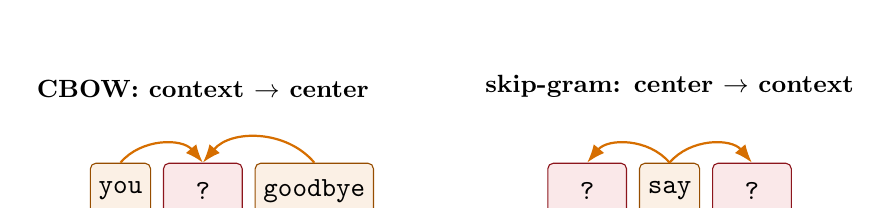
\begin{tikzpicture}[node distance=1.5mm]
\node[tok=attc] (a1) {you}; \node[tok=hotc,right=of a1,minimum width=10mm] (a2) {?}; \node[tok=attc,right=of a2] (a3) {goodbye};
\draw[ar=attc,bend left=50] (a1.north) to (a2.north); \draw[ar=attc,bend right=50] (a3.north) to (a2.north);
\node[lab,font=\bfseries\small,above=7mm of a2] {CBOW: context $\to$ center};
\node[tok=hotc,minimum width=10mm,right=22mm of a3] (b1) {?}; \node[tok=attc,right=of b1] (b2) {say}; \node[tok=hotc,right=of b2,minimum width=10mm] (b3) {?};
\draw[ar=attc,bend right=50] (b2.north) to (b1.north); \draw[ar=attc,bend left=50] (b2.north) to (b3.north);
\node[lab,font=\bfseries\small,above=7mm of b2] {skip-gram: center $\to$ context};
\end{tikzpicture}

\end{center}
\begin{itemize}[leftmargin=1.2em]
\item \textbf{gram}: 그리스어로 ``쓰인 것, 글자''. 연속한 $n$개의 단어 (또는 글자) 묶음을 $n$-gram이라 한다. $1$개는 unigram, $2$개는 bigram (\w{the cat}), $3$개는 trigram이다.
\item \textbf{skip}: 사이의 단어를 \textbf{건너뛴} 쌍도 묶음으로 본다는 뜻이다. 윈도우 크기가 $2$이면 가운데 단어는 바로 옆 단어뿐 아니라 한 칸 건너의 단어와도 짝이 된다.
\end{itemize}
\end{remarkbox}

% =================================================
\section{큰 어휘를 위한 word2vec}\label{sec:fast}
% =================================================

\subsection{어디가 느린가}

어휘가 $100$만 개이고 $H=100$이라고 하자 (\figref{big_vocab}).

\tfig{big_vocab}{어휘가 $100$만 개일 때의 CBOW 모델과 두 병목}

\begin{enumerate}[label=\arabic*.]
\item \textbf{입력 쪽}: 원핫 벡터 (길이 $100$만)와 $W_{\text{in}}$ ($100$만 $\times100$)의 곱. 원핫 벡터는 하나만 빼고 $0$인데도 곱셈을 모두 한다.
\item \textbf{출력 쪽}: $\vect h$와 $W_{\text{out}}$ ($100\times100$만)의 곱으로 점수 $100$만 개를 계산하고, $100$만 개에 대한 softmax를 계산한다. 정답은 하나인데 모든 단어의 점수가 필요하다.
\end{enumerate}

\subsection{입력 쪽: Embedding 층}

원핫 벡터와 행렬의 곱은 행 하나를 꺼내는 것이었다. 그러니 곱하지 말고 \textbf{행을 바로 꺼내면} 된다 (\figref{embedding_lookup}).

\tfig{embedding_lookup}{Embedding 층: 단어 ID로 $W_{\text{in}}$의 행을 바로 꺼낸다}

이 일을 하는 층이 \textbf{Embedding} 층이다. PyTorch에서는 \texttt{nn.Embedding(V, H)}이고, 단어 ID를 넣으면 그 행을 돌려준다.
원핫 벡터를 만들 필요가 없고, 역전파에서도 꺼낸 행에만 gradient가 전달된다.
계산 결과는 원핫 벡터를 곱하는 것과 똑같다. 즉 Embedding 층은 ``원핫 입력을 받는 bias 없는 Linear 층''을 빠르게 계산하는 방법이다.

\subsection{출력 쪽: 네거티브 샘플링}

\textbf{다중 분류를 이진 분류로.}
``가운데 단어는 $100$만 개 중 무엇인가?''라고 묻는 대신, ``가운데 단어는 \w{say}인가? (예/아니오)''라고 묻는다.
그러면 \w{say}의 점수 하나만 계산하면 된다. $W_{\text{out}}$에서 \w{say}에 해당하는 벡터와 $\vect h$의 내적이 점수이고, sigmoid로 확률을 만든다 (\figref{negsample_one}):
\begin{equation}
P(\text{정답이 } \w{say})=\sigma(\vect h\cdot\vect w^{\text{out}}_{\w{say}}),\qquad \sigma(x)=\frac1{1+e^{-x}} .
\end{equation}
\tfig{negsample_one}{정답 단어 하나의 점수만 계산한다}

\textbf{이진 분류의 cross-entropy.}
출력 $y=\sigma(\text{점수})$를 ``예''의 확률로 보면, ``아니오''의 확률은 $1-y$이다.
정답 레이블을 $t$ (``예''이면 $1$, ``아니오''이면 $0$)라고 하면 cross-entropy는
\begin{equation}
\loss=-\big(t\log y+(1-t)\log(1-y)\big)\label{eq:bce}
\end{equation}
이다 ($\log$는 자연로그). $t$는 $1$ 아니면 $0$이므로 두 항 중 하나만 남는다:
\begin{equation}
t=1\text{ 이면 }\ \loss=-\log y,\qquad t=0\text{ 이면 }\ \loss=-\log(1-y).\label{eq:bce_cases}
\end{equation}
어느 쪽이든 loss는 \textbf{정답 쪽 확률}의 $-\log$이다.
다중 분류의 cross-entropy도 정답 클래스의 확률의 $-\log$였다. 이진 분류는 클래스가 ``예''와 ``아니오'' 두 개인 경우일 뿐이다.
정답 쪽 확률이 $1$에 가까우면 loss는 $0$에 가깝고, $0$에 가까우면 loss가 커진다. 예를 들어 $-\log0.9=0.105$, $-\log0.1=2.303$이다.
가운데 단어가 정말 \w{say}이면 $t=1$이므로 loss는 $-\log\sigma(\vect h\cdot\vect w^{\text{out}}_{\w{say}})$이다.

\textbf{오답도 가르쳐야 한다.}
정답에 대해서만 학습하면, 신경망은 모든 단어에 ``예''라고 답해도 된다. 오답 단어에는 ``아니오''라고 답하도록 학습시켜야 한다.
그러나 오답 $999{,}999$개를 모두 쓰면 다시 느려진다. 그래서 오답 몇 개 (보통 $5$--$10$개)만 \textbf{무작위로 뽑아} 쓴다. 이것이 \textbf{네거티브 샘플링}~\cite{mikolov2013b}이다 (\figref{negsample_pn}).

\tfig{negsample_pn}{정답 (\w{say})의 출력은 $1$에, 무작위로 뽑은 오답 (\w{you}, \w{hello})의 출력은 $0$에 가까워지도록 학습한다}

\textbf{한 학습 예의 loss.}
맥락 하나에 대해 이진 분류를 $K+1$번 한다: 정답 단어 하나 ($t=1$)와 오답 $K$개 ($t=0$).
\eqnref{bce_cases}의 두 경우를 그대로 쓰면 정답의 loss는 $-\log\sigma(\vect h\cdot\vect w^{\text{out}}_{\text{정답}})$,
오답 $k$의 loss는 $-\log\big(1-\sigma(\vect h\cdot\vect w^{\text{out}}_{\text{오답}_k})\big)$이다.
이 $K+1$개를 더한 것이 한 학습 예의 loss이다:
\begin{equation}
\loss=-\log\sigma(\vect h\cdot\vect w^{\text{out}}_{\text{정답}})-\sum_{k=1}^{K}\log\big(1-\sigma(\vect h\cdot\vect w^{\text{out}}_{\text{오답}_k})\big).\label{eq:negloss}
\end{equation}
첫 항을 줄이려면 정답 단어의 점수를 올려야 하고, 둘째 항을 줄이려면 오답 단어의 점수를 내려야 한다.
\figref{negsample_loss}에 세 출력이 $0.9$, $0.2$, $0.1$일 때의 계산을 그렸다 (설명을 위해 정한 값).
정답의 loss는 $-\log0.9=0.105$, 오답의 loss는 $-\log(1-0.2)=0.223$과 $-\log(1-0.1)=0.105$이고, 합은 $0.434$이다.

\tfig{negsample_loss}{정답 하나와 오답 둘의 cross-entropy를 더해 한 학습 예의 loss를 만든다}

계산량이 어휘 크기와 상관없이 $K+1$개 단어로 줄었다.

\textbf{오답은 어떻게 뽑는가.}
말뭉치에서 자주 나오는 단어일수록 자주 뽑는다. 드문 단어는 실제로도 드물게 나오므로 오답으로 연습할 필요가 적다.
다만 빈도 그대로 쓰지 않고 $0.75$제곱을 해서 다시 정규화한다:
\begin{equation}
P'(w)=\frac{P(w)^{0.75}}{\sum_{w'}P(w')^{0.75}} .
\end{equation}
그러면 드문 단어도 조금 더 뽑힌다. 예를 들어 확률 $(0.7,\ 0.29,\ 0.01)$은 $(0.642,\ 0.332,\ 0.027)$이 된다.
PTB의 단어에 적용한 결과는 \figref{neg_sampling_dist}에 있다.

\fig[0.85]{figures/neg_sampling_dist.png}{PTB에서 단어의 빈도 $P(w)$와 $0.75$제곱 후의 확률 (세로축은 로그 눈금). 흔한 단어는 덜, 드문 단어는 더 뽑힌다}

\needspace{18\baselineskip}
\subsection{PTB로 학습하기}

\texttt{cbow\_ptb.py}의 모델이다. $W_{\text{in}}$과 $W_{\text{out}}$을 모두 \texttt{nn.Embedding}으로 두고, 단어 $K$개 (정답 하나와 오답들)의 점수를 한 번에 계산한다.

\begin{lstlisting}
class CBOW(nn.Module):
    def __init__(self, V, H):
        super().__init__()
        self.W_in = nn.Embedding(V, H)               # row i = vector of word i (input side)
        self.W_out = nn.Embedding(V, H)              # row i = vector of word i (output side)
        nn.init.normal_(self.W_in.weight, std=0.01)
        nn.init.normal_(self.W_out.weight, std=0.01)

    def forward(self, ctx, words):                   # ctx (B, 10), words (B, K) -> scores (B, K)
        h = self.W_in(ctx).mean(dim=1)               # (B, H): average of the context vectors
        return (self.W_out(words) * h[:, None, :]).sum(dim=-1)   # dot products h . w_out
\end{lstlisting}

학습 루프에서는 맥락마다 정답 단어 하나와 무작위로 뽑은 오답 $5$개를 나란히 놓고, 정답에는 $1$, 오답에는 $0$을 목표로 준다.

\begin{lstlisting}
neg = torch.multinomial(p_neg, len(b) * n_neg, replacement=True).view(len(b), n_neg)
words = torch.cat([target[b, None], neg], dim=1)                       # (B, 6)
labels = torch.zeros_like(words, dtype=torch.float32); labels[:, 0] = 1
scores = model(contexts[b], words)
loss = F.binary_cross_entropy_with_logits(scores, labels, reduction="sum") / len(b)
\end{lstlisting}

\texttt{F.binary\_cross\_entropy\_with\_logits}는 점수에 sigmoid를 적용하고 \eqnref{bce}의 cross-entropy를 계산한다.
\texttt{reduction="sum"}으로 모든 학습 예의 loss를 더한 뒤 \texttt{len(b)}로 나누므로, 결과는 \eqnref{negloss} (정답 $1$개와 오답 $5$개의 loss의 합)의 미니배치 평균이다.

윈도우 크기 $5$ (좌우 다섯 단어씩), $H=100$, 오답 $5$개, 미니배치 $100$, Adam (학습률 $10^{-3}$)으로 $10$ epoch 학습했다.
GPU (RTX 3050)에서 약 $6$분이 걸렸다. loss (정답 하나와 오답 다섯 개의 loss의 합)는 첫 epoch 끝의 $2.260$에서 마지막 epoch 끝의 $1.478$로 줄었다 (\figref{cbow_ptb_loss}).

\fig[0.5]{figures/cbow_ptb_loss.png}{PTB로 학습한 CBOW의 loss}

학습된 $W_{\text{in}}$의 행으로 비슷한 단어를 찾으면:

\begin{center}
\begin{tabular}{@{}ll@{}}
\toprule
단어 & 가장 비슷한 단어 (코사인 유사도) \\
\midrule
\w{you} & \w{we} ($0.732$), \w{i} ($0.667$), \w{your} ($0.608$), \w{they} ($0.576$), \w{anything} ($0.571$) \\
\w{year} & \w{month} ($0.855$), \w{week} ($0.784$), \w{summer} ($0.753$), \w{spring} ($0.744$), \w{decade} ($0.696$) \\
\w{car} & \w{luxury} ($0.613$), \w{truck} ($0.597$), \w{window} ($0.589$), \w{vehicle} ($0.583$), \w{cars} ($0.572$) \\
\w{toyota} & \w{coated} ($0.633$), \w{honda} ($0.627$), \w{chevrolet} ($0.611$), \w{f-14} ($0.611$), \w{weyerhaeuser} ($0.606$) \\
\bottomrule
\end{tabular}
\end{center}

\w{year}에 기간을 나타내는 단어들이 모인 것처럼 대부분 그럴듯하지만, \w{toyota}의 \w{coated}처럼 엉뚱한 단어도 섞여 있다. PTB는 약 $93$만 단어로, 단어 벡터를 학습하기에는 작은 말뭉치이다.

\subsection{단어 벡터로 유추 문제 풀기}

word2vec의 단어 벡터는 비슷한 단어끼리 모일 뿐 아니라, 단어 사이의 \textbf{관계}도 벡터의 차이로 나타낸다고 알려져 있다.
``\w{man} : \w{woman} = \w{king} : ?''를 벡터로 쓰면 $\vect v_{\w{woman}}-\vect v_{\w{man}}+\vect v_{\w{king}}$에 가장 가까운 단어를 찾는 문제이다 (\figref{analogy}).

\tfig{analogy}{\w{man}에서 \w{woman}으로 가는 벡터를 \w{king}에 더하면 \w{queen}에 가까워지기를 기대한다}

PTB로 학습한 벡터로 풀어 보면 (\texttt{cbow\_ptb.py}의 4번 셀)

\begin{center}
\footnotesize
\begin{tabular}{@{}ll@{}}
\toprule
문제 & 답의 후보 (코사인 유사도) \\
\midrule
\w{take} : \w{took} = \w{go} : ? & \w{went} ($0.669$), \w{came} ($0.591$), \w{ran} ($0.585$), \w{got} ($0.551$), \w{began} ($0.541$) \\
\w{car} : \w{cars} = \w{child} : ? & \w{parents} ($0.630$), \w{women} ($0.627$), \w{males} ($0.619$), \w{children} ($0.616$), \w{adults} ($0.614$) \\
\w{man} : \w{king} = \w{woman} : ? & \w{bike} ($0.614$), \w{max} ($0.566$), \w{lexington} ($0.554$), \w{horse} ($0.550$), \w{artist} ($0.545$) \\
\w{good} : \w{better} = \w{bad} : ? & \w{greater} ($0.616$), \w{less} ($0.568$), \w{more} ($0.561$), \w{rather} ($0.523$), \w{ever} ($0.487$) \\
\bottomrule
\end{tabular}
\end{center}

과거형 (\w{went})은 맞혔고, 복수형은 사람을 나타내는 복수 명사들 사이에 \w{children}이 $4$번째로 나왔다.
\w{king}--\w{queen}과 \w{better}--\w{worse}는 풀지 못했다. 경제 신문 기사인 PTB의 약 $93$만 단어 중에 \w{king}은 $43$번, \w{queen}은 $7$번밖에 나오지 않는다.
수십억 단어의 말뭉치로 학습한 단어 벡터는 이런 문제를 훨씬 잘 푼다. 말뭉치의 크기와 내용이 단어 벡터의 품질을 정한다.

\subsection{단어 벡터와 지금의 언어모델}\label{sec:w2vtoday}

word2vec은 2013년에 나왔다~\cite{mikolov2013a,mikolov2013b}. ChatGPT 같은 지금의 언어모델과는 어떤 관계일까?
결론부터 말하면, 단어마다 벡터 하나를 정해 두는 word2vec 그대로의 모습은 많이 쓰이지 않는다.
그러나 이 장의 부품과 생각은 지금의 언어모델 \textbf{안에} 그대로 들어 있다.

\textbf{왜 밀집 벡터인가.} 원핫 벡터에서는 모든 단어가 서로 똑같이 다르다. \w{cat}과 \w{dog}의 거리나 \w{cat}과 \w{stock}의 거리가 같다.
밀집 벡터에서는 비슷하게 쓰이는 단어가 가까이 있다. 그래서 학습 데이터에서 \w{the cat sat}만 본 신경망도, \w{dog}의 벡터가 \w{cat}과 가까우면 \w{the dog sat}을 비슷하게 처리할 수 있다.
신경망이 글을 다룰 때 밀집 벡터에서 시작하는 이유이고, 이것은 지금도 같다.

\textbf{지금도 그대로 쓰는 것.}
\begin{itemize}[leftmargin=1.5em]
\item \textbf{Embedding 층.} ChatGPT를 포함한 모든 언어모델의 첫 층은 \ref{sec:fast}절의 \texttt{nn.Embedding}이다. 입력한 글을 토큰 (단어 조각, \ref{sec:gpt}절)으로 자르고, 토큰 ID로 표의 행을 꺼낸다.
마지막 층은 $W_{\text{out}}$처럼 벡터와 각 토큰의 벡터의 내적으로 점수를 낸다 (\figref{w2v_vs_gpt}). GPT-2~\cite{radford2019}처럼 첫 층과 마지막 층이 같은 행렬을 함께 쓰는 모델도 있다.
\item \textbf{정답 없는 글로 학습하기.} word2vec은 사람이 정답을 달지 않은 글에서 문제와 정답을 만들었다 (\ref{sec:cbowtrain}절의 학습 데이터). GPT의 사전학습 (pre-training)도 같다. 차이는 맞히는 것이 가운데 단어가 아니라 다음 토큰이라는 것이다.
\item \textbf{먼저 배우고 옮겨 쓰기.} 큰 말뭉치로 먼저 학습한 것을 정답이 붙은 데이터가 적은 과제에 옮겨 쓰는 방법을 \textbf{전이 학습} (transfer learning)이라 한다. 처음에는 단어 벡터를 옮겨 썼고, 지금은 사전학습한 언어모델 전체를 옮겨 쓴다.
\item \textbf{벡터로 바꾸어 비슷한 것 찾기.} 글을 벡터로 바꾸고 코사인 유사도로 비슷한 것을 찾는 방법은 지금 검색과 추천의 기본이다.
대화형 언어모델이 문서를 찾아 보고 답하는 방법 (RAG, retrieval-augmented generation)~\cite{lewis2020}도 이것이다. 문서들을 미리 벡터로 바꾸어 저장해 두고 (vector database), 질문의 벡터와 코사인 유사도가 큰 문서를 찾아 언어모델에 함께 넣는다.
\end{itemize}

\tfig{w2v_vs_gpt}{CBOW와 GPT. 입력 쪽 Embedding과 출력 쪽 점수 계산은 같고, 가운데의 ``평균''이 Transformer 블록으로 바뀌었다}

\textbf{형태를 바꾸어 쓰는 것.}
\begin{itemize}[leftmargin=1.5em]
\item \textbf{단어 벡터에서 문장, 문서 벡터로.} RAG에서 쓰는 벡터는 단어 하나가 아니라 문장이나 문서 전체의 벡터이다. 이 벡터를 만드는 \textbf{임베딩 모델}은 Transformer이다 (\ref{sec:transformer}절).
\item \textbf{네거티브 샘플링에서 대조 학습으로.} 네거티브 샘플링은 맞는 쌍 (맥락, 정답)의 점수는 높이고 무작위로 뽑은 틀린 쌍의 점수는 낮추었다.
같은 생각을 문장에 쓰면, 뜻이 같은 문장 쌍 (질문과 그 답이 있는 문서 등)은 가깝게, 무작위 문장 쌍은 멀게 학습한다. 이것을 \textbf{대조 학습} (contrastive learning)이라 하고, 임베딩 모델 대부분이 이렇게 학습한다.
\item \textbf{글이 아닌 것으로.} 그림과 그 설명 글을 같은 공간의 가까운 벡터로 만드는 모델 (CLIP~\cite{radford2021})도 대조 학습으로 학습한다. 그림을 글로 찾거나 글로 그림을 만드는 모델의 기초이다.
그림도 함께 읽는 언어모델은 그림을 조각으로 나누어 토큰 벡터와 같은 크기의 벡터로 바꾸어 넣는다. 단어든 그림 조각이든 ``벡터 하나''로 만들어 넣는다는 점에서 이 장의 연장이다.
\item \textbf{단어가 아닌 열에 word2vec을.} 사용자가 차례로 본 상품이나 들은 노래의 열을 문장처럼 보고 word2vec을 학습하면, 함께 소비되는 상품끼리 가까운 벡터를 얻는다. 추천 시스템에서 쓰는 방법이다 (item2vec~\cite{barkan2016}). 그래프 위를 걸어 다닌 노드의 열에 쓰면 node2vec~\cite{grover2016}이다.
\end{itemize}

\textbf{이제 거의 쓰지 않는 것.}
\begin{itemize}[leftmargin=1.5em]
\item \textbf{고정된 단어 벡터를 다른 모델의 입력으로 넣기.} 2013--2017년에는 word2vec이나 GloVe~\cite{pennington2014}로 미리 학습한 단어 벡터를 RNN의 입력으로 쓰는 것이 표준이었다.
2018년 BERT~\cite{devlin2019}, GPT~\cite{radford2018} 이후로는 사전학습한 Transformer 전체를 가져다 쓴다. 고정된 단어 벡터는 \w{river bank}의 \w{bank}와 \w{bank account}의 \w{bank}를 구별하지 못하기 때문이다 (\ref{sec:gpt}절).
\item \textbf{PPMI와 SVD.} 지금은 실용보다 이해를 위한 출발점이다. 다만 둘은 생각보다 가깝다. 네거티브 샘플링을 쓴 skip-gram은 사실상 PMI 행렬을 분해하는 것과 같다는 결과가 알려져 있다~\cite{levy2014}.
세어서 만드는 방법 (\ref{sec:count}절)과 맞히면서 배우는 방법 (\ref{sec:w2v}절)은 같은 정보를 다른 길로 얻는 셈이다.
\end{itemize}
고정된 단어 벡터도 완전히 사라지지는 않았다. 계산이 가볍고 빨라서, 휴대전화 안에서 하는 간단한 글 분류나 언어 판별, 그리고 여러 시대의 말뭉치에서 단어 뜻의 변화나 편향을 재는 연구에 쓰인다.

\begin{center}
\begin{tabular}{@{}p{38mm}p{100mm}@{}}
\toprule
이 장의 내용 & 지금의 언어모델에서 \\
\midrule
Embedding 층 & 모든 언어모델의 첫 층 (토큰 ID $\to$ 벡터) \\
$W_{\text{out}}$의 점수 & 마지막 층에서 다음 토큰의 점수 \\
정답 없는 글로 학습 & 사전학습 (다음 토큰 맞히기) \\
네거티브 샘플링 & 대조 학습 (임베딩 모델, CLIP) \\
코사인 유사도로 찾기 & 검색, 추천, RAG \\
단어마다 고정된 벡터 & 문맥에 따라 달라지는 벡터로 대체 (\ref{sec:gpt}절) \\
\bottomrule
\end{tabular}
\end{center}

\textbf{남은 문제.} 단어 벡터는 단어 \textbf{하나}의 표현이다. 문장을 나타내려고 단어 벡터들을 평균하면, \ref{sec:cbowtrain}절에서 본 것처럼 단어의 순서가 사라진다.
\w{dog bites man}과 \w{man bites dog}은 같은 단어들로 되어 있지만 뜻이 다르다.
순서가 있는 단어의 열을 읽는 방법 (\ref{sec:rnn}절의 RNN)과, 문맥을 보고 단어의 벡터를 바꾸는 방법 (\ref{sec:transformer}절의 Transformer)이 이 문제를 푼다.

\begin{mlbox}[1--4절 정리]
\begin{itemize}[leftmargin=1.5em]
\item 단어의 의미는 주변 단어 (맥락)로 정해진다 (분포 가설).
\item 통계 기반: 동시발생 행렬을 세고, PPMI로 흔한 단어의 영향을 줄이고, SVD로 차원을 줄인다.
\item 추론 기반 (word2vec): 맥락으로 가운데 단어를 맞히는 신경망 (CBOW)을 학습하면, 입력 쪽 가중치 $W_{\text{in}}$의 행이 단어 벡터가 된다.
\item CBOW는 맥락의 단어 벡터를 평균하므로 맥락 안의 순서를 보지 못한다 (bag-of-words).
\item 큰 어휘에서는 원핫 곱 대신 Embedding 층 (행 꺼내기)을, softmax 대신 네거티브 샘플링 (정답 하나와 오답 몇 개의 이진 분류)을 쓴다.
\item 지금의 언어모델도 Embedding 층으로 시작하고, 정답 없는 글로 사전학습한다. 고정된 단어 벡터 대신 문맥에 따라 달라지는 벡터를 쓰고, 벡터로 비슷한 것을 찾는 방법은 검색과 RAG에 쓰인다.
\item 남은 질문: 단어가 아니라 \textbf{문장}, 즉 순서가 있는 단어의 열은 어떻게 다룰까? (\ref{sec:lm}절부터)
\end{itemize}
\end{mlbox}

% =================================================
\section*{연습문제 (1--4절)}
% =================================================

\begin{enumerate}[label=\arabic*.]
\item 예문 \w{"you say goodbye and i say hello ."}의 동시발생 행렬을 윈도우 크기 $2$로 만들어라.
\item \ref{sec:count}절의 동시발생 행렬 (윈도우 크기 $1$)에서 $\operatorname{PPMI}(\w{hello},\w{.})$를 계산하라. 왜 $\operatorname{PPMI}(\w{say},\w{hello})$보다 큰가?
\item 코사인 유사도는 벡터의 길이를 무시한다. 동시발생 횟수를 그대로 쓸 때 이것이 왜 중요한지 설명하라.
\item 원핫 벡터 $(0,0,1,0)$과 $4\times3$ 행렬 $W$의 곱이 $W$의 셋째 행임을 보여라.
\item CBOW 모델에서 맥락이 네 단어 (윈도우 크기 $2$)이면 은닉층 $\vect h$는 어떻게 계산하는가?
\item 맥락이 (\w{say}, \w{and})인 학습 예와 (\w{and}, \w{say})인 학습 예에서 CBOW의 은닉층 $\vect h$가 같음을 식으로 보여라.
모델이 두 정답에 주는 확률을 $p$, $1-p$라 할 때, 두 예의 loss의 합 $-\log p-\log(1-p)$가 $p=\tfrac12$에서 가장 작음을 보여라.
\item 어휘 $10{,}000$개, $H=100$인 CBOW에서 softmax를 쓸 때와 네거티브 샘플링 (오답 $5$개)을 쓸 때, 학습 예 하나에 계산하는 점수의 수를 비교하라.
\item 확률 $(0.5,\ 0.3,\ 0.2)$에 $0.75$제곱을 적용하여 다시 정규화하라.
\item \w{you say goodbye and i say hello .}에서 윈도우 크기 $2$의 skip-gram이 만드는 (가운데 단어, 맥락 단어) 쌍 중 가운데 단어가 \w{goodbye}인 것을 모두 써라.
\end{enumerate}

\clearpage
% #################################################
\partbanner{문장을 다루는 신경망: RNN}
% #################################################

% =================================================
\section{언어모델}\label{sec:lm}
% =================================================

\subsection{단어 열의 확률}

\ref{sec:w2v}절의 CBOW는 맥락 (앞뒤의 단어)으로 \textbf{가운데} 단어를 맞혔다. 이제 \textbf{앞의 단어들만} 보고 \textbf{다음} 단어를 맞히는 모델을 생각한다 (\figref{p_next}):
\begin{equation}
P(w_t\mid w_1,w_2,\dots,w_{t-1}).
\end{equation}

\tfig{p_next}{앞의 단어들 전체를 맥락으로 다음 단어의 확률을 계산한다}

이 확률을 알면 문장 전체의 확률도 계산할 수 있다. 확률의 곱셈 법칙에 의해
\begin{equation}
P(w_1,\dots,w_m)=P(w_1)\,P(w_2\mid w_1)\,P(w_3\mid w_1,w_2)\cdots P(w_m\mid w_1,\dots,w_{m-1})
\end{equation}
이기 때문이다. 단어 열에 확률을 주는 모델을 \textbf{언어모델}이라 한다.
\begin{itemize}[leftmargin=1.5em]
\item 문장이 얼마나 자연스러운지 평가할 수 있다. 음성 인식이나 번역에서 후보 문장 중 자연스러운 것을 고를 때 쓴다.
\item 다음 단어의 확률에서 단어를 하나 뽑고, 그것을 붙여 다시 다음 단어를 뽑으면 \textbf{문장을 생성}할 수 있다 (\ref{sec:gen}절).
\end{itemize}

\subsection{앞의 단어를 모두 보아야 한다}

CBOW를 언어모델로 쓰려면 맥락을 왼쪽 몇 단어로 바꾸면 된다. 그러나 맥락의 길이가 고정된다. \figref{tom}의 빈칸을 보자.

\tfig{tom}{빈칸을 맞히려면 $18$단어 앞의 \w{Tom}을 기억해야 한다}

답은 \w{Tom}이다. 이것을 맞히려면 훨씬 앞의 단어를 기억해야 한다. 맥락의 길이를 $20$으로 늘리면 가중치도 그만큼 늘어난다.
게다가 CBOW는 맥락의 단어 벡터를 \textbf{평균}하므로 단어의 순서를 잃는다.
\textbf{길이에 제한이 없고 순서를 기억하는} 모델이 필요하다. 그것이 RNN이다.

% =================================================
\section{RNN}\label{sec:rnn}
% =================================================

\subsection{순환하는 신경망}

\textbf{RNN} (recurrent neural network, 순환 신경망)은 한 층의 출력이 다음 시각에 다시 자기 입력으로 들어가는 고리를 가진 신경망이다.
시각 $t$에 단어 벡터 $\vect x_t$가 들어오면, RNN 계층은 바로 전 시각의 $\vect h_{t-1}$과 함께 계산하여 $\vect h_t$를 낸다.
$\vect h_t$는 두 곳으로 간다.
\begin{itemize}[leftmargin=1.5em]
\item 위로: Affine과 softmax를 거쳐 그 시각의 출력 $\vect y_t$ (예: 다음 단어의 확률)가 된다.
\item 오른쪽으로: 다음 시각의 RNN 계층에 $\vect h_{t-1}$로 다시 들어간다.
\end{itemize}
$\vect h_t$는 신경망의 최종 출력이 아니라 중간 층의 출력이다. 고리를 시간 방향으로 펼치면, 같은 층들이 시각마다 한 번씩 쓰이는 긴 신경망이 된다 (\figref{rnn_loop}).

\tfig{rnn_loop}{왼쪽: RNN 계층의 출력 $\vect h_t$는 위의 Affine으로 가고, 다음 시각에 $\vect h_{t-1}$로 다시 들어온다. 오른쪽: 고리를 시간 방향으로 펼친 모습}

각 시각의 계산은
\begin{equation}
\vect h_t=\tanh\big(\vect h_{t-1}W_h+\vect x_tW_x+\vect b\big),\qquad
\vect y_t=\operatorname{softmax}\big(\vect h_tW_{\text{out}}+\vect b_{\text{out}}\big)\label{eq:rnn}
\end{equation}
이다. $W_x$는 입력을, $W_h$는 이전 은닉 상태를 변환하는 가중치이고, $W_{\text{out}}$은 Affine 층의 가중치이다. 모든 시각에 같은 가중치를 쓴다.
$\vect h_t$를 \textbf{은닉 상태}라 한다. 지금까지 읽은 단어들의 정보를 요약한 벡터로, 한 단어를 읽을 때마다 갱신된다.
\begin{itemize}[leftmargin=1.5em]
\item ``은닉''은 데이터에 나타나지 않는다는 뜻이다. 입력 (단어)과 정답 (다음 단어)은 데이터에 있지만, $\vect h_t$에 무엇을 담을지는 아무도 정해 주지 않는다. 다음 단어를 잘 맞히도록 학습하면서 $W_h$, $W_x$가 정한다. MLP의 은닉층 출력과 같은 것이다.
\item 크기는 문장 길이와 상관없이 고정이다 (\texttt{rnnlm\_ptb.py}에서 $100$차원). $3$단어를 읽었든 $300$단어를 읽었든 $100$개의 숫자로 요약해야 하므로, 무엇을 남기고 무엇을 버릴지가 중요하다. 이 한계는 \ref{sec:lstm}절과 \ref{sec:attn}절의 동기가 된다.
\item 예를 들어 \w{Tom} 문제 (\ref{sec:lm}절)를 풀려면 \w{Tom}의 정보가 $18$번의 갱신을 거치는 동안 $\vect h$ 안에 남아 있어야 한다.
\end{itemize}

\textbf{CBOW와 비교하기.} 앞의 두 단어로 다음 단어를 맞히는 CBOW와 RNN을 나란히 쓰면 다음과 같다.
\begin{equation}
\text{CBOW: }\ \vect h=\tfrac12(\vect x_{t-1}+\vect x_t),\qquad
\text{RNN: }\ \vect h_t=\tanh\big(\vect h_{t-1}W_h+\vect x_tW_x+\vect b\big).
\end{equation}
두 경우 모두 다음 단어의 확률은 $\vect h$에 Affine과 softmax를 붙여 얻는다.
RNN에서 $\vect y_t$를 정하는 것은 $\vect h_t$이고, $\vect h_t$는 현재 단어 $\vect x_t$와 그 앞의 문맥 전체를 담은 $\vect h_{t-1}$로 만든다.
앞의 모든 문맥을 벡터 하나로 들고 다니기 위해 만든 것이 은닉 상태이다.
\begin{center}
\begin{tabular}{@{}lp{50mm}p{62mm}@{}}
\toprule
 & CBOW (앞의 두 단어) & RNN \\
\midrule
보는 단어 & 정해진 개수 ($2$개) & 앞의 모든 단어 \\
단어를 합치는 방법 & 평균 (모든 단어에 같은 가중치 $1/2$) & $\vect x_t$는 $W_x$로, 앞 문맥 $\vect h_{t-1}$은 $W_h$로 변환해 더하고 $\tanh$ \\
단어의 순서 & 잃는다 (\w{a b}와 \w{b a}가 같다) & 남는다. 먼 단어일수록 $W_h$와 $\tanh$를 더 여러 번 거친다 \\
\bottomrule
\end{tabular}
\end{center}
\eqnref{rnn}의 첫 식을 한 번 펼치면 $\vect h_t=\tanh\big(\tanh(\vect h_{t-2}W_h+\vect x_{t-1}W_x+\vect b)W_h+\vect x_tW_x+\vect b\big)$이다.
단어마다 거치는 변환이 다르므로, 같은 단어라도 위치에 따라 $\vect h_t$에 주는 영향이 다르다. 단순한 가중합이 아니고, 각 단어의 영향은 학습된 $W_h$, $W_x$와 단어들의 값에 따라 정해진다.

$\vect h_t$를 구하려면 $\vect h_{t-1}$이 먼저 있어야 하므로, RNN은 단어를 \textbf{처음부터 한 번에 하나씩} 순서대로 처리한다.
처음 상태 $\vect h_0$은 보통 영벡터이다. RNN 계층 하나의 계산은 \figref{rnn_cell}에 있다.

\tfig{rnn_cell}{RNN 계층 하나의 계산 그래프}

\begin{remarkbox}[RNN은 언제 왜 만들어졌나]
보통의 신경망 (MLP, CNN)은 \textbf{정해진 크기}의 입력을 받는다. 그러나 문장, 음성, 주가처럼 시간 순서가 있는 데이터는 길이가 제각각이고, 순서가 의미를 가진다.
입력을 하나씩 받으면서 지금까지 본 것을 \textbf{상태}로 기억하는 신경망이 RNN이다. 다음 단어 예측만을 위해 만든 것이 아니라, 순서가 있는 데이터 일반을 위한 것이다.
\begin{itemize}[leftmargin=1.2em]
\item 1986년: Rumelhart, Hinton, Williams가 역전파를 발표하며 순환하는 신경망도 시간 방향으로 펼쳐 학습할 수 있음을 보였다~\cite{rumelhart1986}. 같은 해 Jordan은 출력을 다시 입력으로 넣는 신경망을 제안했다~\cite{jordan1986}.
\item 1990년: Elman이 은닉 상태를 다시 입력으로 넣는, \eqnref{rnn}의 형태의 RNN (Elman network)을 제안했다~\cite{elman1990}. 그의 실험이 바로 \textbf{다음 단어 맞히기}였고, 학습된 은닉 상태에서 명사와 동사가 저절로 나뉘었다. 같은 해 Werbos가 BPTT를 정리했다~\cite{werbos1990}.
\item 1991--1994년: Hochreiter, Bengio 등이 긴 열에서 기울기가 사라지는 문제를 밝혔다~\cite{hochreiter1991,bengio1994} (\ref{sec:lstm}절). 1997년 Hochreiter와 Schmidhuber가 이를 줄인 LSTM을 발표했다~\cite{hochreiter1997}.
\item 2010년대: GPU와 큰 데이터로 RNN이 실용화되었다. Mikolov의 RNN 언어모델 (2010)~\cite{mikolov2010}이 $n$-gram을 앞섰고, LSTM이 음성 인식 (2013)~\cite{graves2013}과 기계 번역 (seq2seq, 2014)~\cite{sutskever2014}에서 최고 성능을 냈다.
\item 2017년 이후: 언어 처리에서는 Transformer (\ref{sec:transformer}절)가 RNN을 대신했다. RNN은 시계열 예측이나 실시간 처리처럼 입력이 하나씩 들어오는 곳에 여전히 쓰이고, 고정 크기 상태로 긴 열을 읽는 아이디어는 최근의 상태공간 모델 (예: Mamba~\cite{gu2023})로 이어졌다.
\end{itemize}
쓰임에 따라 출력을 받는 위치가 다르다. 시각마다 출력을 받으면 언어모델이나 품사 태깅이고, 마지막 은닉 상태만 쓰면 문장 분류 (예: 감정 분석)이며, 한 RNN의 마지막 상태를 다른 RNN에 넘기면 번역 (\ref{sec:gen}절의 seq2seq)이 된다.
\end{remarkbox}

\subsection{시간 방향의 역전파}

펼친 RNN은 그냥 긴 신경망이므로 역전파도 똑같이 하면 된다. 이것을 \textbf{BPTT} (backpropagation through time)라 한다.
\figref{bptt}는 $T$개 시각을 펼친 모습이다. 각 시각의 $\vect h_t$ 위의 상자는 Affine, softmax, cross-entropy를 묶은 것으로, 그 시각의 loss $\loss_t$를 낸다. 전체 loss는 $\loss=\frac1T\sum_t\loss_t$이다.

\tfig{bptt}{BPTT. 순전파 (검은색)에서 $\vect h_t$는 위의 loss와 다음 시각의 RNN 계층 두 곳으로 간다. 역전파 (빨간색)에서는 두 곳에서 온 gradient가 $+$에서 더해져 RNN 계층으로 들어간다}

\textbf{두 곳에서 온 gradient를 더한다.} 순전파에서 $\vect h_t$는 두 곳에 쓰인다. 위의 Affine (그 시각의 loss $\loss_t$)과 다음 시각의 RNN 계층이다.
계산 그래프에서 한 값이 두 곳으로 갈라지면, 역전파에서는 두 곳에서 온 gradient를 더한다. 그래서
\begin{equation}
\frac{\partial\loss}{\partial\vect h_t}
=\underbrace{\frac1T\frac{\partial\loss_t}{\partial\vect h_t}}_{\text{위의 loss에서}}
+\underbrace{\Big(\frac{\partial\loss}{\partial\vect h_{t+1}}\odot\big(1-\vect h_{t+1}^2\big)\Big)W_h\T}_{\text{다음 시각에서}}\label{eq:bptt}
\end{equation}
이다. 둘째 항은 \eqnref{rnn}의 $\vect h_{t+1}=\tanh(\vect h_tW_h+\cdots)$를 거슬러 온 것이다. $\odot$는 원소별 곱이고, $1-\vect h_{t+1}^2$ (성분마다 제곱)은 $\tanh$의 미분이다.
마지막 시각 $T$에는 다음 시각이 없으므로 첫째 항만 있다. 그래서 역전파는 $t=T$에서 시작해 $t=T-1,\dots,1$의 순서로, 순전파와 반대 방향으로 진행한다.
$W_x$, $W_h$, $\vect b$는 모든 시각이 함께 쓰므로, 그 gradient는 시각마다 구한 것을 모두 더한 것이다.

\textbf{Truncated BPTT: 블록씩 끊어서 학습하기.} 문장이 길면 펼친 신경망도 길어진다. 말뭉치 전체를 하나로 펼치면 계산량과 메모리가 감당할 수 없다.
그래서 시간 방향으로 $T$단어 (예: $35$단어)씩 끊어 블록을 만들고, 블록 하나씩 학습한다 (\figref{tbptt}).
\begin{enumerate}[leftmargin=1.5em]
\item 블록 1: $\vect x_1,\dots,\vect x_T$를 순전파해 $\loss_1,\dots,\loss_T$를 구한다. 블록 안에서만 \eqnref{bptt}로 역전파하고, 가중치를 한 번 갱신한다.
\item 블록 2: 블록 1의 마지막 은닉 상태 $\vect h_T$를 시작 상태로 받아 $\vect x_{T+1},\dots,\vect x_{2T}$를 순전파하고, 역시 블록 안에서만 역전파해 갱신한다. $\vect h_T$는 값만 받을 뿐, 블록 1로 gradient를 보내지 않는다.
\item 블록 3, 4, \dots도 같은 방법으로 차례로 학습한다.
\end{enumerate}

\tfig{tbptt}{Truncated BPTT. 블록마다 $T$개 시각을 순전파하고 그 안에서만 역전파한 뒤 가중치를 한 번 갱신한다. 다음 블록은 $\vect h_T$의 값만 받는다}

순전파는 끊지 않으므로 문맥이 블록을 넘어 이어진다. 역전파는 블록 안에서만 하므로 계산량과 메모리가 $T$에 비례한다.
가중치 갱신 한 번이 $T$개 시각을 처리하는 셈이다. 대신 $T$단어보다 먼 단어 사이의 관계는 gradient로 직접 배우지 못한다.
이것을 \textbf{Truncated BPTT}라 한다. PyTorch에서는 다음 블록에 넘기는 은닉 상태에 \texttt{.detach()}를 쓴다. 값은 그대로 두고 계산 그래프만 끊는 것이다.

\textbf{미니배치로 읽기.} 위의 블록 학습은 긴 단어 열 하나를 처음부터 차례로 읽는다. GPU에서 여러 열을 동시에 계산하려면, 말뭉치를 $B$조각으로 잘라 $B$개의 행으로 놓고 각 행을 $T$단어씩 나란히 읽는다 (\figref{batchify}).
\begin{itemize}[leftmargin=1.5em]
\item 각 행이 \figref{tbptt}의 블록 학습을 따로 한다. 같은 RNN 계층이 $B$개 행을 동시에 계산하고, 은닉 상태도 행마다 하나씩 $B$개이다.
\item $(B,T)$ 크기의 조각 하나가 미니배치 하나이다. 정답은 같은 조각을 오른쪽으로 한 단어 민 것이고, loss는 $B\times T$개 위치의 cross-entropy의 평균이다.
\item 한 미니배치를 다 읽은 뒤의 은닉 상태 (행마다 하나씩, $B$개)를 다음 미니배치의 \textbf{같은 행}의 시작 상태로 넘긴다. 각 행은 말뭉치의 이어진 부분이므로, 행마다 문맥이 이어진다.
\end{itemize}

\tfig{batchify}{말뭉치를 $B=20$개 행으로 자르고, 각 행을 $T=35$단어씩 나란히 읽는다. 숫자는 PTB에서 단어의 위치이다}

\texttt{rnnlm\_ptb.py}는 $B=20$, $T=35$를 쓴다. PTB 학습 데이터 ($929{,}589$단어)는 $46{,}479$단어짜리 행 $20$개가 되고 (남는 $9$단어는 버린다), 한 epoch은 $\lceil46{,}479/35\rceil=1{,}328$번의 갱신이다.

\subsection{RNN 언어모델}

RNN으로 언어모델을 만들면 \figref{rnnlm}처럼 된다. 각 시각에 단어를 Embedding으로 벡터로 바꿔 RNN에 넣고, RNN의 출력에 Affine (Linear) 층과 softmax를 붙여 다음 단어의 확률을 낸다.

\tfig{rnnlm}{\w{you say goodbye and ...}를 처리하는 RNN 언어모델. 각 시각의 정답은 다음 단어이다}

\textbf{입력은 무엇인가.} 모델이 받는 것은 단어 ID이고, Embedding 층이 ID에 해당하는 행을 꺼내 $\vect x_t$로 만든다.
원핫 벡터에 행렬을 곱해도 그 행 하나가 나오므로 (\ref{sec:fast}절), 원핫 벡터를 넣는 것과 계산은 같고 더 빠를 뿐이다.

\textbf{시각마다 예측한다.} 첫 시각에는 \w{you} 하나만 보고 다음 단어를 예측하고, 둘째 시각에는 \w{you say}를 요약한 $\vect h_2$로 예측한다.
시각 $t$의 예측은 $1$번째부터 $t$번째 단어까지만 본다. 첫 단어 하나로 한 예측은 정보가 적어 틀리기 쉽지만, 이것도 loss에 들어간다.

정답은 CBOW 때처럼 (\ref{sec:w2v}절) 말뭉치에서 만든다. 입력 단어열을 한 칸 민 것이 정답이다. loss는 모든 시각의 cross-entropy의 평균이다.
은닉 상태가 앞의 단어들을 기억하므로, \w{say} 다음에 \w{goodbye}와 \w{hello} 중 무엇이 올지를 그 앞의 단어들로 구별할 수 있다.

\textbf{$\vect h_t$는 단어가 아니다.} $\vect h_t$는 RNN 계층의 출력이자 다음 시각으로 넘어가는 은닉 상태이지만, 예측한 단어는 아니다.
$\vect h_t$에 Affine과 softmax를 붙여야 어휘 전체에 대한 확률분포 (예: \w{say} $0.6$, \w{hello} $0.1$, \dots)가 나온다.
다음 시각으로 넘어가는 것은 이 확률이 아니라 $\vect h_t$이다.

\textbf{학습할 때와 생성할 때.} 다음 시각의 입력 $\vect x_{t+1}$으로 무엇을 넣는지가 다르다.
\begin{itemize}[leftmargin=1.5em]
\item 학습: 정답 문장이 있으므로 정답 단어를 그대로 넣는다. 시각 $1$의 예측이 틀렸어도 시각 $2$에는 정답 \w{say}가 들어간다 (\textbf{teacher forcing}~\cite{williams1989}).
그래서 $T$개 시각의 예측이 한꺼번에 나오고, 모두 loss에 들어간다.
\item 생성: 정답이 없으므로 확률분포에서 단어를 하나 뽑아 다음 입력으로 넣고, 다시 다음 단어를 뽑는다.
끝을 나타내는 기호가 나오거나 정한 길이가 될 때까지 반복한다 (\ref{sec:gen}절).
\end{itemize}
한 번에 예측하는 것은 다음 단어 하나이지만, 뽑은 단어를 다시 넣는 반복으로 문장이 만들어진다. GPT도 같은 방식으로 한 토큰씩 생성한다 (\ref{sec:gpt}절).

PyTorch에서는 세 층을 차례로 쓰면 된다 (\texttt{rnnlm\_ptb.py}의 2번 셀). \texttt{nn.RNN}은 $T$개 시각을 한꺼번에 받아 모든 시각의 은닉 상태를 낸다.
호출이 한 번일 뿐, 안에서는 시각 순서대로 계산한다.
\texttt{cell}로 RNN과 \ref{sec:lstm}절의 LSTM 중 하나를 고른다.

\begin{lstlisting}
class RNNLM(nn.Module):
    def __init__(self, V, D=100, H=100, cell="lstm"):
        super().__init__()
        layer = nn.LSTM if cell == "lstm" else nn.RNN
        self.embed = nn.Embedding(V, D)                  # word ID -> vector
        self.rnn = layer(D, H, batch_first=True)
        self.out = nn.Linear(H, V)

    def forward(self, x, state=None):                    # x: (B, T) word IDs
        h, state = self.rnn(self.embed(x), state)        # h: (B, T, H), all hidden states
        return self.out(h), state                        # (B, T, V): scores of the next word
\end{lstlisting}

\texttt{state}는 마지막 시각의 은닉 상태이다. 이것을 받아 두었다가 다음 미니배치를 넣을 때 함께 넘긴다. 학습의 한 epoch은 다음과 같다 (3번 셀).

\begin{lstlisting}
state = None                             # no state yet: the layer starts from zeros
for k in range(0, train.size(1) - 1, T):
    x, y = train[:, k:k + T], train[:, k + 1:k + 1 + T]      # y: x shifted by one word
    x = x[:, :y.size(1)]
    if state is not None:
        state = detach(state)            # truncated BPTT: keep the values, cut the graph
    logits, state = model(x, state)      # starts from the last state of the previous block
    loss = F.cross_entropy(logits.reshape(-1, V), y.reshape(-1))
    opt.zero_grad()
    loss.backward()
    nn.utils.clip_grad_norm_(model.parameters(), 1.0)    # gradient clipping
    opt.step()
\end{lstlisting}

\texttt{train}은 말뭉치를 $(20,\ 46479)$ 크기로 놓은 것이다. 앞 블록의 상태를 이어받으므로, 블록의 첫 단어도 실제로는 그 앞의 문맥을 안다. 상태가 $\vect 0$에서 시작하는 것은 말뭉치의 맨 처음뿐이다.
\texttt{detach}가 Truncated BPTT의 ``역전파만 끊기''이고, \texttt{clip\_grad\_norm\_}은 \ref{sec:lstm}절에서 설명한다.

\begin{remarkbox}[Embedding 층과 word2vec의 관계]
RNN 언어모델의 첫 층인 Embedding은 \ref{sec:w2v}절의 $W_{\text{in}}$과 같은 ``단어 ID $\to$ 벡터'' 표이다. 이 표를 정하는 방법은 두 가지이다.
\begin{itemize}[leftmargin=1.2em]
\item word2vec으로 미리 학습한 단어 벡터를 초기값으로 넣는다. 학습 데이터가 적은 과제에서, 큰 말뭉치에서 얻은 단어의 지식을 빌려 쓰는 방법이다.
\item 무작위 값에서 시작해 RNN과 함께 학습한다. RNN 언어모델도 ``앞 단어로 다음 단어 맞히기''라는 예측을 학습하므로, word2vec과 같은 원리로 Embedding의 행이 단어의 분산 표현이 된다.
\end{itemize}
이 노트의 코드 (\texttt{rnnlm\_ptb.py})와 지금의 큰 언어모델은 두 번째 방법을 쓴다.

\medskip
\textbf{앞의 문맥이 섞이는데도 왜 단어의 표현인가.}
Embedding 표를 CBOW에서처럼 $W_{\text{in}}$ ($V\times D$, $D$는 단어 벡터의 크기로 코드에서 $100$)이라 하자. 단어 $w$가 들어오면 $\vect x_t$는 $W_{\text{in}}$의 $w$번째 행이고,
$\vect h_t=\tanh\big(\vect h_{t-1}W_h+\vect x_tW_x+\vect b\big)$ (\eqnref{rnn})에서 ``어떤 단어인가''는 $\vect x_t$로만 들어온다. $W_h$, $W_x$, $\vect b$는 모든 단어가 함께 쓰고, $\vect h_{t-1}$은 문맥이다.
\begin{itemize}[leftmargin=1.2em]
\item $\vect h_{t-1}$은 $\vect x_t$를 바꾸지 않고 옆에 더해질 뿐이다. 문맥이 섞이는 것은 $\vect h_t$이고, $W_{\text{in}}$의 행은 문맥과 상관없이 같다.
\item 단어 $w$가 어떤 문맥에 나오든 그 행에 gradient가 온다. 비슷한 자리에 쓰이고 뒤에 비슷한 단어가 오는 단어 (예: \w{cat}과 \w{dog})는 비슷하게 다뤄야 loss가 작으므로, 행이 서로 가까워진다.
\item 앞의 문맥이 없는 첫 단어 ($\vect h_0=\vect 0$)에서는 한 단어만 보고 다음 단어를 맞히는 문제가 되지만, 그것은 특수한 경우일 뿐이다. 행은 대부분 문맥이 있는 상태에서 학습된다.
\end{itemize}
원핫 벡터를 Embedding 없이 RNN에 바로 넣으면 $\vect x_tW_x$가 $W_x$ ($V\times H$)의 한 행이 되어, $W_x$의 행이 같은 역할을 한다.
$W_{\text{in}}$의 행은 문맥과 상관없는 \textbf{고정된 표현}, $\vect h_t$는 문맥 속에서 읽은 \textbf{문맥 표현}이다 (\ref{sec:w2vtoday}절, \ref{sec:gpt}절).
Mikolov 등 (2013)~\cite{mikolov2013c}은 RNN 언어모델의 이 행들로 \w{king} $-$ \w{man} $+$ \w{woman} $\approx$ \w{queen} 같은 유추가 됨을 보였고, 이것이 word2vec으로 이어졌다.
\end{remarkbox}

\subsection{퍼플렉서티}

언어모델의 성능은 \textbf{퍼플렉서티} (perplexity)로 잰다:
\begin{equation}\label{eq:ppl}
\text{perplexity}=\exp(\loss),\qquad \loss=-\frac1N\sum_{n=1}^N\log P(\text{정답}_n).
\end{equation}
$N$은 검증용 (또는 테스트용) 글의 단어 수이고, $P(\text{정답}_n)$은 $n$번째 위치에서 모델이 실제 다음 단어에 준 확률이다.

\textbf{$\loss$는 학습에 쓴 cross-entropy loss이다.} 정답이 원핫 벡터 $\vect t$, 모델의 출력이 $\vect y$일 때 cross-entropy는 $-\sum_k t_k\log y_k$이다.
$\vect t$는 정답 자리만 $1$이므로 항 하나만 남아 $-\log P(\text{정답})$이 된다. 부호도 같다.
\eqnref{ppl}의 $\loss$는 이것을 $N$개 위치에서 평균한 것으로, 학습 때의 loss를 학습에 쓰지 않은 글에서 잰 값이다.
$0<P\le1$이므로 $-\log P\ge0$이고, $\loss\ge0$, 퍼플렉서티 $\ge1$이다. 모든 정답에 확률 $1$을 주어야 $\loss=0$, 퍼플렉서티 $1$이 된다.
$\exp$는 증가함수이므로 $\loss$가 작을수록 퍼플렉서티도 작고, 작을수록 좋은 모델이다.

\textbf{왜 $\exp$를 취하는가.} $\loss$를 그대로 써도 모델의 순위는 같다. $\exp$를 취하는 것은 숫자에 뜻을 주기 위해서이다.
\begin{itemize}[leftmargin=1.5em]
\item \textbf{확률의 역수의 기하평균.} 로그의 평균에 $\exp$를 취하면 기하평균이 된다:
\begin{equation}\label{eq:ppl_geo}
\exp(\loss)=\Big(\prod_{n=1}^N\frac{1}{P(\text{정답}_n)}\Big)^{1/N}.
\end{equation}
정답의 확률이 항상 $0.8$이면 퍼플렉서티는 $1/0.8=1.25$, 항상 $0.2$이면 $5$이다 (\figref{perplexity_example}).
\item \textbf{후보의 수.} 모델이 매번 정답을 포함한 $k$개의 단어에 똑같이 $1/k$씩 주고 나머지에는 $0$을 준다면 퍼플렉서티는 정확히 $k$이다.
그래서 퍼플렉서티는 ``모델이 매 시각 몇 개의 후보 사이에서 망설이는 것과 같은가''로 읽는다. 어휘가 $V$개이고 아무것도 모르면 (모든 단어에 $1/V$) 퍼플렉서티는 $V$이다.
$\loss$는 로그 단위라 $\loss=4.94$라고만 하면 감이 오지 않지만, 퍼플렉서티로 바꾸면 $e^{4.94}\approx140$, 즉 ``후보 $140$개 중 하나를 고르는 만큼 헷갈린다''가 된다.
\item \textbf{왜 기하평균인가.} 글 전체의 확률은 각 단어의 확률의 곱이다: $P(\text{글})=\prod_nP(\text{정답}_n)$. 따라서 \eqnref{ppl_geo}는 $P(\text{글})^{-1/N}$, 즉 모델이 테스트용 글 전체에 준 확률을 단어 하나당으로 바꾸어 뒤집은 값이다.
예를 들어 두 단어에 $0.8$, $0.2$를 주었으면 $P(\text{글})=0.16$이고 퍼플렉서티는 $0.16^{-1/2}=2.5$이다. 역수 $1.25$와 $5$의 산술평균 $3.125$와 다르다.
\end{itemize}

\textbf{어디에서 온 개념인가.} 정보이론이다. 섀넌 (Shannon)은 불확실성을 엔트로피로 정의했다~\cite{shannon1948}:
$H=-\sum_xp(x)\log_2p(x)$ (단위: bit).
$k$개가 똑같이 나올 수 있으면 $H=\log_2k$이므로, 거꾸로 $2^H$는 ``같은 불확실성을 가진 균등분포의 경우의 수''이다.
퍼플렉서티는 이 $2^H$를 실제 글과 모델의 cross-entropy로 잰 것이다. 로그의 밑을 $2$로 하면 $2^{\loss}$, $e$로 하면 $e^{\loss}$로, 값은 같다.
1970년대 음성 인식 연구에서 Jelinek 등이 ``다음 단어를 맞히는 과제가 얼마나 어려운가''를 재는 척도로 이 이름을 붙였다~\cite{jelinek1977}.

퍼플렉서티는 같은 어휘 (같은 토큰 단위)로 잴 때만 비교할 수 있다. 어휘가 크거나 단위가 단어인지 토큰 (\ref{sec:gpt}절)인지에 따라 같은 모델도 값이 달라진다.

\fig[0.9]{figures/perplexity_example.png}{\w{you} 다음에 \w{say}가 정답일 때. 모델 1은 $0.8$, 모델 2는 $0.2$의 확률을 주었다}

% =================================================
\section{LSTM: 오래 기억하는 RNN}\label{sec:lstm}
% =================================================

\subsection{RNN의 문제: 기울기 소실과 폭발}

\w{Tom} 문제 (\ref{sec:lm}절)를 풀려면, 마지막 단어에서 계산한 loss의 gradient가 $18$단어 앞까지 전달되어야 한다 (\figref{tom_grad}).
그래야 ``\w{Tom}의 정보를 은닉 상태에 남겨 두라''는 학습 신호가 그 시각의 가중치에 닿는다.

\tfig{tom_grad}{정답 \w{Tom}의 gradient가 시간을 거슬러 앞의 단어까지 전달되어야 한다}

\textbf{한 단계를 거슬러 갈 때.} $\vect h_t=\tanh(\vect h_{t-1}W_h+\vect x_tW_x+\vect b)$ (\eqnref{rnn})를 역전파하면
\begin{equation}
\frac{\partial\loss}{\partial\vect h_{t-1}}=\Big(\frac{\partial\loss}{\partial\vect h_t}\odot\big(1-\vect h_t^2\big)\Big)W_h\T\label{eq:rnn_back}
\end{equation}
이다 (\eqnref{bptt}의 둘째 항). $\odot$는 원소별 곱이고, $1-\vect h_t^2$ (성분마다 제곱)은 $\tanh$의 미분 $\tanh'(a)=1-\tanh^2(a)$이다.
$18$단어를 거슬러 가면 \eqnref{rnn_back}의 계산을 $18$번 반복하므로, $\tanh$의 미분과 $W_h\T$를 $18$번 곱하게 된다.

\begin{itemize}[leftmargin=1.5em]
\item $\tanh$의 미분은 $1$ 이하이고, 입력이 $0$에서 멀어지면 $0$에 가깝다. 여러 번 곱하면 gradient가 점점 작아진다.
\item 같은 행렬 $W_h\T$를 여러 번 곱한다. $W_h$의 특잇값 (\ref{sec:count}절)이 모두 $1$보다 작으면 gradient는 지수적으로 작아지고, $1$보다 큰 특잇값이 있으면 지수적으로 커질 수 있다 (\figref{rnn_grad_norm}).
\end{itemize}

\fig[0.9]{figures/rnn_grad_norm.png}{gradient에 $W_h\T$를 $20$번 곱할 때의 크기 (\texttt{figures\_extra.py}의 3번 셀). $W_h$가 회전행렬의 $1.3$배 (특잇값이 모두 $1.3$)이면 $20$번 뒤 $232.8$로 커지고 (왼쪽), $0.7$배이면 $0.001$로 작아진다 (오른쪽)}

gradient가 커지는 \textbf{기울기 폭발}은 비교적 쉽게 막는다. gradient의 크기가 기준을 넘으면 줄이는 \textbf{gradient clipping}이다 (PyTorch: \texttt{nn.utils.clip\_grad\_norm\_}).
모든 가중치의 gradient를 이어 붙인 벡터를 $\vect g$, 기준을 $\theta$라 하면
\begin{equation}
\|\vect g\|>\theta\ \text{이면}\quad \vect g\leftarrow\frac{\theta}{\|\vect g\|}\,\vect g
\end{equation}
이다. 방향은 그대로 두고 크기만 $\theta$로 줄인다. \texttt{rnnlm\_ptb.py}는 $\theta=1$을 쓴다.

gradient가 사라지는 \textbf{기울기 소실}은 그렇게 해결되지 않는다.
가중치의 gradient는 시각마다의 기여를 모두 더한 것인데, 먼 과거에서 오는 기여만 $0$에 가까워진다. loss는 여전히 줄지만, 가중치는 가까운 몇 단어만 보고 맞히는 쪽으로만 학습된다.
멀리 떨어진 단어 사이의 관계 (\w{Tom}을 기억하기)는 배우지 못한다. gradient 전체를 키워도 가까운 단어의 기여가 함께 커질 뿐이므로, RNN의 구조 자체를 바꿔야 한다. 그것이 LSTM이다.

이 문제는 Hochreiter (1991)~\cite{hochreiter1991}와 Bengio 등 (1994)~\cite{bengio1994}이 분석했다. Gradient clipping은 Mikolov가 RNN 언어모델에 쓰기 시작했고~\cite{mikolov2012}, Pascanu 등 (2013)~\cite{pascanu2013}이 기울기 폭발과 함께 정리했다.

\subsection{LSTM의 구조}

\textbf{LSTM} (long short-term memory)은 은닉 상태 $\vect h$ 외에 \textbf{기억 셀} $\vect c$라는 통로를 하나 더 갖는다.
$\vect c$는 LSTM 계층 안에서만 다음 시각으로 전달되고, 밖으로 나가는 출력은 여전히 $\vect h$이다 (\figref{lstm_c}).

\textbf{왜 통로가 하나 더 필요한가.} RNN은 매 시각 $\vect h_t=\tanh(\cdots)$로 은닉 상태 전체를 \textbf{새로 계산}한다. 오래 남겨야 할 정보도 매번 $W_h$와 $\tanh$를 거치며 조금씩 변하고, gradient도 그 길로만 돌아간다.
LSTM의 기억 셀은 메모장처럼 다룬다. 통째로 다시 쓰지 않고, 필요한 성분만 \textbf{지우고} (forget), \textbf{적고} (input), 필요할 때 \textbf{읽어 낸다} (output). 손대지 않은 성분은 그대로 다음 시각으로 넘어간다.

\tfig{lstm_c}{LSTM은 기억 셀 $\vect c$를 따로 가진다}

LSTM의 핵심은 \textbf{게이트}이다. 게이트는 정보를 ``얼마나'' 통과시킬지를 $0$과 $1$ 사이의 값으로 정한다. 수도꼭지를 얼마나 열지 정하는 것과 같다.
열림 정도는 sigmoid로 만들고, 그 값도 학습으로 정해진다 (\figref{gate}).

\tfig{gate}{게이트: 벡터의 성분마다 $0$--$1$ 사이의 값을 곱해 얼마나 통과시킬지 정한다}

이제 부품을 하나씩 더하며 LSTM을 만든다. 순서는 기억 셀 $\to$ output 게이트 $\to$ forget 게이트 $\to$ 새 기억 $\vect g$ $\to$ input 게이트이다.
단계마다 ``그 부품이 없으면 무엇이 곤란한가''를 먼저 보고, 그것을 해결하는 부품을 더한다. 그림에서 빨간 점선이 그 단계에서 더한 부분이다.

\subsection{기억 셀: 오래 담아 두는 곳}\label{sec:lstmcell}

먼저 게이트 없이 기억 셀만 둔다 (\figref{lstm_s1}).
\begin{itemize}[leftmargin=1.5em]
\item 기억 셀 $\vect c_t$는 지금까지 읽은 내용 가운데 \textbf{오래 간직할 것}을 담는다. 이전 기억 $\vect c_{t-1}$, 지금 단어 $\vect x_t$, 직전 출력 $\vect h_{t-1}$로 새 기억 $\vect c_t$를 만든다. 그 방법 (그림의 \w{update})은 뒤의 게이트들이 채운다.
\item 은닉 상태는 기억 셀에서 \textbf{읽어 낸 것}이다: $\vect h_t=\tanh(\vect c_t)$. $\vect c_t$는 덧셈이 쌓여 커질 수 있으므로 $\tanh$로 $-1$과 $1$ 사이로 누른다. RNN의 $\vect h_t$와 같은 범위이다.
\item $\vect h_t$는 RNN과 똑같이 위의 Affine 층과 다음 시각으로 간다. $\vect c_t$는 다음 시각의 LSTM으로만 간다.
\end{itemize}
\textbf{역할 나누기.} RNN의 은닉 상태 $\vect h_t$는 두 가지 일을 한꺼번에 했다.
\begin{itemize}[leftmargin=1.5em]
\item \textbf{지금의 출력}: Affine 층이 $\vect h_t$로 다음 단어를 맞힌다.
\item \textbf{기억}: $\vect h_t$를 다음 시각으로 넘겨 앞의 문맥을 전한다.
\end{itemize}
두 일은 서로 부딪친다. 다음 단어를 맞히려면 지금 필요한 정보가 $\vect h_t$에 드러나 있어야 하고, 기억하려면 지금은 필요 없어도 나중에 필요한 정보 (\w{Tom})를 간직해야 한다.
벡터 하나로 둘을 다 하므로, 오래 간직할 정보도 매 시각 $\tanh(\vect h_{t-1}W_h+\vect x_tW_x+\vect b)$로 다시 계산되며 조금씩 변한다.

LSTM은 \textbf{기억하는 일을 기억 셀 $\vect c$에 전담시킨다}. $\vect c$는 정보를 오래 \textbf{보관}하는 곳이고, $\vect h$는 그 가운데 지금 쓰려고 \textbf{꺼낸 것}이다.
$\vect h_t$도 여전히 다음 시각으로 가지만 역할이 다르다. 기억을 보관하는 것은 $\vect c$이고, $\vect h_{t-1}$은 다음 시각에 게이트와 새 내용을 계산할 때 ``직전에 무엇을 꺼내 썼는가''를 알려 주는 입력이다.
이렇게 나누면 기억의 경로를 단순하게 만들 수 있다. 뒤에서 보듯 $\vect c$의 경로에는 $W_h$도 $\tanh$도 없고 원소별 곱과 덧셈만 있다.
그래서 손대지 않은 기억은 그대로 남고, gradient도 그 길로 먼 과거까지 전달된다 (\ref{sec:lstmgrad}절).

\textbf{이름의 뜻.} 이름의 단기 기억, 장기 기억은 인지심리학에서 사람의 기억을 나누는 말을 신경망 연구가 빌려 쓴 것이다.
LSTM을 제안한 논문~\cite{hochreiter1997}도 신경망 안의 기억을 다음 두 종류로 나누는 데서 시작한다.

\begin{center}
\begin{tabular}{@{}llll@{}}
\toprule
& 담는 곳 & 바뀌는 때 & 남는 범위 \\
\midrule
장기 기억 & 가중치 $W$ & 학습할 때 (천천히) & 학습이 끝나면 고정되고, 모든 글에 쓰인다 \\
단기 기억 & 활성값 ($\vect h$, $\vect c$) & 입력이 들어올 때마다 & 지금 읽는 글 안에서만 \\
\bottomrule
\end{tabular}
\end{center}

``앞에 \w{Tom}이 나왔다''처럼 지금 읽는 글의 내용은 가중치가 아니라 활성값에 담기고, 새 글을 읽을 때는 보통 영벡터에서 다시 시작한다.
그러니 단기 기억은 $\vect h$나 $\vect c$ 하나를 가리키는 말이 아니라 기억의 \textbf{종류}이고, $\vect h$와 $\vect c$는 둘 다 단기 기억이다.
둘 가운데 \textbf{오래 가는 것은 $\vect c$}이다. $\vect c$는 손대지 않으면 거의 그대로 다음 시각으로 넘어가지만, $\vect h$는 매 시각 $\vect c$에서 새로 꺼내 만든다 ($\vect h_t=\tanh(\vect c_t)$, 다음 절에서 output 게이트를 곱한다).
RNN에서는 단기 기억이 $\vect h$ 하나뿐이었고, 매 시각 $W_h$와 $\tanh$를 거치며 몇 단어 만에 흐려졌다.
LSTM은 단기 기억 $\vect c$가 오래 가게 만들었다. 그래도 $\vect c$는 가중치가 아니라 활성값이므로 장기 기억은 아니다.
그래서 long short-term memory, ``오래 가는 단기 기억''이다.

빌린 것은 이름뿐이고, 구조는 사람의 기억을 흉내 내서 나온 것이 아니다.
Hochreiter는 RNN의 기울기가 시간을 거슬러 가며 지수적으로 줄어드는 것을 분석했고~\cite{hochreiter1991}, 그 해결책으로 이전 값에 $1$을 곱해 그대로 넘기는 셀을 두었다~\cite{hochreiter1997}.
이 길에서는 오차가 줄지도 커지지도 않고 그대로 흐르므로 constant error carousel이라 불렀다. 게이트는 그 셀에 정보가 아무 때나 들고 나지 않도록 입구와 출구에 붙인 것이다.
처음 LSTM의 기억 셀이 $\vect c_t=\vect c_{t-1}+\vect i\odot\vect g$였던 것이 이 때문이다 (\ref{sec:lstmsum}절의 역사).

\tfig{lstm_s1}{1단계: 기억 셀 $\vect c$만 둔다. $\vect c_t$를 만드는 방법 (\w{update})은 뒤의 게이트들이 채우고, 출력은 $\vect h_t=\tanh(\vect c_t)$이다}

\subsection{output 게이트: 기억에서 무엇을 꺼낼까}

\textbf{문제.} $\vect h_t=\tanh(\vect c_t)$이면 기억한 것이 \textbf{모두, 매 시각} 출력된다.
\w{Tom} 문제에서 ``주어는 \w{Tom}''이라는 기억은 마지막 \w{to} 다음에서야 필요하다. 그 사이 $18$단어 동안 다음 단어를 맞힐 때는 쓸모가 없고, 오히려 방해가 된다. $\vect h_t$는 Affine 층이 다음 단어를 맞히는 데에도, 다음 시각의 계산에도 쓰이기 때문이다.

\textbf{해결.} 성분마다 얼마나 내보낼지 정하는 게이트 $\vect o$를 둔다 (\figref{lstm_s2}):
\begin{equation}
\vect o=\sigma(\vect x_tW_x^{(o)}+\vect h_{t-1}W_h^{(o)}+\vect b^{(o)}),\qquad \vect h_t=\vect o\odot\tanh(\vect c_t).
\end{equation}
\begin{itemize}[leftmargin=1.5em]
\item $o_k\approx1$이면 $k$번째 기억을 그대로 내보내고, $o_k\approx0$이면 내보내지 않는다. 중간 값이면 그만큼 줄여서 내보낸다.
\item $\vect o$는 지금 단어 $\vect x_t$와 직전 출력 $\vect h_{t-1}$로 계산한다. ``지금 상황에서 어떤 기억이 쓸모 있는가''를 매 시각 다시 판단한다는 뜻이다.
\item $\vect o$는 $\vect h_t$에만 곱하고 $\vect c_t$는 건드리지 않는다. \textbf{내보내지 않는 것은 지우는 것이 아니다.} $o_k\approx0$인 기억도 $\vect c$ 안에 그대로 남아 있다가, 필요한 시각에 $o_k$가 열리면 나온다.
\end{itemize}

\tfig{lstm_s2}{2단계: output 게이트 $\vect o$를 더한다. 기억 $\tanh(\vect c_t)$ 가운데 지금 쓸 성분만 $\vect h_t$로 내보낸다}

\subsection{forget 게이트: 무엇을 지울까}

\textbf{문제.} 기억은 언젠가 지워야 한다. 문장이 끝나고 새 문장이 시작되거나 이야기의 주어가 \w{Mary}로 바뀌면, ``주어는 \w{Tom}''은 더 이상 맞는 정보가 아니다.
지우지 못하면 오래된 정보가 새 정보와 섞이고, 덧셈이 계속 쌓여 $\vect c$의 값도 커진다.

\textbf{해결.} 이전 기억 $\vect c_{t-1}$에 성분마다 남길 비율 $\vect f$를 곱한다 (\figref{lstm_s3}):
\begin{equation}
\vect f=\sigma(\vect x_tW_x^{(f)}+\vect h_{t-1}W_h^{(f)}+\vect b^{(f)}),\qquad \vect c_t=\vect f\odot\vect c_{t-1}\quad(\text{이 단계까지}).
\end{equation}
\begin{itemize}[leftmargin=1.5em]
\item $f_k\approx1$이면 $k$번째 기억을 그대로 남기고, $f_k\approx0$이면 지운다. 이름은 forget이지만 값은 ``남길 비율''이다. $1$이 ``잊지 마라''이다.
\item 성분마다, 시각마다 따로 정한다. 마침표나 새 주어를 읽은 시각에는 주어를 담은 성분의 $f_k$가 닫히고, 다른 성분은 그대로 남을 수 있다.
\item $f_k$가 $0.9$ 정도로 계속 머물면 그 기억은 매 시각 $10\%$씩 서서히 흐려진다. 얼마나 오래 기억할지도 학습으로 정해진다.
\end{itemize}

\tfig{lstm_s3}{3단계: forget 게이트 $\vect f$를 더한다. 이전 기억 $\vect c_{t-1}$의 성분마다 남길 비율을 곱한다}

\subsection{새 기억 \texorpdfstring{$\vect g$}{g}: 무엇을 적을까}

\textbf{문제.} 지금까지의 LSTM은 기억을 남기거나 지울 수만 있다. 지금 읽은 단어 $\vect x_t$의 정보를 기억에 \textbf{적는} 방법이 없다.

\textbf{해결.} 적을 내용 $\vect g$를 만들어 남긴 기억에 \textbf{더한다} (\figref{lstm_s4}):
\begin{equation}
\vect g=\tanh(\vect x_tW_x^{(g)}+\vect h_{t-1}W_h^{(g)}+\vect b^{(g)}),\qquad \vect c_t=\vect f\odot\vect c_{t-1}+\vect g\quad(\text{이 단계까지}).
\end{equation}
\begin{itemize}[leftmargin=1.5em]
\item $\vect g$의 식은 RNN의 \eqnref{rnn} 첫 식과 같다. 지금 단어와 직전 출력을 섞어 만든, RNN이었다면 그대로 은닉 상태가 되었을 내용이다.
\item 게이트와 달리 $\tanh$를 쓴다. $\vect g$는 ``얼마나''가 아니라 \textbf{내용}이므로 양수도 음수도 될 수 있어야 한다. 크기는 $-1$과 $1$ 사이로 제한된다.
\item 덮어쓰지 않고 \textbf{더한다}. RNN은 매 시각 은닉 상태를 통째로 새로 계산했지만, LSTM은 남긴 기억 위에 새 내용을 얹는다. 이 덧셈이 기울기가 사라지지 않는 이유가 된다 (\ref{sec:lstmgrad}절).
\end{itemize}

\tfig{lstm_s4}{4단계: 새 기억 $\vect g$를 더한다. 지금 단어에서 만든 내용을 남긴 기억에 더해 적는다}

\subsection{input 게이트: 적을 내용을 얼마나 받아들일까}

\textbf{문제.} 이대로면 모든 단어의 $\vect g$가 매 시각 기억에 더해진다. \w{Tom}과 마지막 \w{to} 사이의 $18$단어 대부분은 오래 기억할 필요가 없는데, 그 내용이 계속 쌓이면 \w{Tom}의 기억이 묻힌다.

\textbf{해결.} $\vect g$에 성분마다 받아들일 비율 $\vect i$를 곱해서 더한다 (\figref{lstm_full}):
\begin{equation}
\vect i=\sigma(\vect x_tW_x^{(i)}+\vect h_{t-1}W_h^{(i)}+\vect b^{(i)}),\qquad \vect c_t=\vect f\odot\vect c_{t-1}+\vect i\odot\vect g.
\end{equation}
\begin{itemize}[leftmargin=1.5em]
\item $i_k\approx0$이면 지금 단어는 $k$번째 기억에 아무것도 적지 않는다. 그 기억은 지금 단어로부터 \textbf{보호된다}.
\item 역할이 나뉜다. $\vect g$는 \textbf{무엇을} 적을지 (내용, $-1$--$1$), $\vect i$는 \textbf{얼마나} 적을지 (세기, $0$--$1$)를 정한다. 내용을 만드는 일과 적을지 말지 판단하는 일을 따로 학습한다.
\item forget 게이트와 짝을 이룬다. $f_k\approx0$, $i_k\approx1$이면 옛 기억을 지우고 새 내용으로 바꿔 적는다. $f_k\approx1$, $i_k\approx0$이면 옛 기억을 그대로 지킨다.
\end{itemize}

\tfig{lstm_full}{5단계: input 게이트 $\vect i$를 더해 완성한 LSTM 계층의 계산 그래프. 위의 굵은 선이 기억 셀의 경로이다}

\subsection{정리: LSTM의 식}\label{sec:lstmsum}

다섯 단계를 모으면 LSTM 계층의 식이다. 네 식 모두 같은 입력 $(\vect x_t,\vect h_{t-1})$으로 계산한다:
\begin{align}
\vect f&=\sigma(\vect x_tW_x^{(f)}+\vect h_{t-1}W_h^{(f)}+\vect b^{(f)}) &&\text{forget 게이트: 이전 기억을 얼마나 남길까}\label{eq:lstm_f}\\
\vect i&=\sigma(\vect x_tW_x^{(i)}+\vect h_{t-1}W_h^{(i)}+\vect b^{(i)}) &&\text{input 게이트: 새 정보를 얼마나 더할까}\\
\vect o&=\sigma(\vect x_tW_x^{(o)}+\vect h_{t-1}W_h^{(o)}+\vect b^{(o)}) &&\text{output 게이트: 기억을 얼마나 내보낼까}\\
\vect g&=\tanh(\vect x_tW_x^{(g)}+\vect h_{t-1}W_h^{(g)}+\vect b^{(g)}) &&\text{새로 기억할 내용}\label{eq:lstm_g}
\end{align}
그리고 기억 셀과 출력을 갱신한다 ($\odot$는 원소별 곱):
\begin{equation}
\boxed{\;\vect c_t=\vect f\odot\vect c_{t-1}+\vect i\odot\vect g,\qquad \vect h_t=\vect o\odot\tanh(\vect c_t)\;}\label{eq:lstm_c}
\end{equation}
식~\eqref{eq:lstm_f}--\eqref{eq:lstm_g}의 네 식은 모양이 \eqnref{rnn}의 첫 식과 같고 가중치만 따로 쓴다. 위첨자 $(f)$, $(i)$, $(o)$, $(g)$는 어느 식의 가중치인지를 표시한 것이고, 네 결과는 모두 $\vect h$와 같은 $H$차원 벡터이다.
네 부품의 역할을 표로 모으면 다음과 같다.

\begin{center}
\begin{tabular}{@{}llll@{}}
\toprule
부품 & 활성화 & 값의 범위 & 하는 일 \\
\midrule
forget 게이트 $\vect f$ & sigmoid & $0$--$1$ & 이전 기억 $\vect c_{t-1}$을 성분마다 얼마나 남길까 \\
새 기억 $\vect g$ & $\tanh$ & $-1$--$1$ & 지금 단어에서 무엇을 적을까 (내용) \\
input 게이트 $\vect i$ & sigmoid & $0$--$1$ & $\vect g$를 성분마다 얼마나 적을까 \\
output 게이트 $\vect o$ & sigmoid & $0$--$1$ & 기억 $\tanh(\vect c_t)$를 성분마다 얼마나 내보낼까 \\
\bottomrule
\end{tabular}
\end{center}

\textbf{한 시각을 숫자로 따라가기.} $H=3$인 기억 셀에서 한 시각의 계산을 보자. 게이트 값은 설명을 위해 정한 것이다.

\begin{center}
\begin{tabular}{@{}lrrrl@{}}
\toprule
& 성분 1 & 성분 2 & 성분 3 & \\
\midrule
이전 기억 $\vect c_{t-1}$ & $2.0$ & $-1.0$ & $0.5$ & \\
forget $\vect f$ & $0.99$ & $0.01$ & $0.5$ & \\
$\vect f\odot\vect c_{t-1}$ & $1.98$ & $-0.01$ & $0.25$ & 남긴 기억 \\
새 기억 $\vect g$ & $0.5$ & $0.8$ & $-0.6$ & \\
input $\vect i$ & $0.01$ & $0.99$ & $0.5$ & \\
$\vect i\odot\vect g$ & $0.005$ & $0.792$ & $-0.3$ & 적는 내용 \\
$\vect c_t$ & $1.985$ & $0.782$ & $-0.05$ & 새 기억 셀 \\
$\tanh(\vect c_t)$ & $0.963$ & $0.654$ & $-0.05$ & \\
output $\vect o$ & $0.02$ & $0.97$ & $0.5$ & \\
$\vect h_t$ & $0.019$ & $0.634$ & $-0.025$ & 출력 \\
\bottomrule
\end{tabular}
\end{center}

\begin{itemize}[leftmargin=1.5em]
\item 성분 1: 지키고 (forget $0.99$), 적지 않고 (input $0.01$), 내보내지 않는다 (output $0.02$). 기억은 $2.0$에서 $1.985$로 거의 그대로이지만 출력은 $0.019$로 거의 $0$이다. 지금은 쓰지 않지만 나중을 위해 간직하는 기억이다.
\item 성분 2: 옛 기억 $-1.0$을 지우고 (forget $0.01$) 새 내용 $0.8$을 적은 뒤 (input $0.99$) 바로 내보낸다 (output $0.97$). 지금 단어의 정보를 지금 쓴다.
\item 성분 3: 모든 게이트가 $0.5$이다. 옛 기억의 절반과 새 내용의 절반이 섞이고, 그 절반을 내보낸다.
\end{itemize}
RNN이었다면 세 성분 모두 $\tanh(\cdots)$로 새로 계산되어, 성분 1처럼 값을 그대로 간직하는 일이 어렵다.
성분 1이 \ref{sec:lstmcell}절에서 말한 ``오래 가는 단기 기억''의 모습이다. 기억은 $\vect c$에 남아 있고, 지금의 $\vect h$에는 드러나지 않는다.

\textbf{예: \w{Tom} 문제.} 학습이 잘 되었다면 다음처럼 동작할 수 있다.
\w{Tom}을 읽을 때 input 게이트가 열려, $\vect c$의 어떤 성분에 ``주어는 \w{Tom}''이라는 정보가 적힌다.
그 뒤 $18$단어 동안 그 성분의 forget 게이트는 $1$ 가까이, input 게이트는 $0$ 가까이 있어 값이 그대로 유지된다.
\w{to}를 읽고 다음 단어로 사람 이름이 와야 할 때 output 게이트가 그 성분을 열어 $\vect h$로 내보낸다.
어느 성분을 언제 열지는 사람이 정하지 않는다. 다음 단어를 잘 맞히도록 학습하면서 게이트의 가중치가 정해진다.

\textbf{게이트를 어떻게 이해할까.} $\vect c_t$와 $\vect h_t$의 각 성분은 지금까지 읽은 글의 어떤 \textbf{특징}을 담는다. 게이트는 그 특징들에 성분마다 다른 비율을 곱해 남길지, 적을지, 내보낼지를 조절한다.
CNN에서 채널 (특징맵)마다 다른 가중치를 곱하는 것과 비슷하다. 다만 세 가지를 짚어 두어야 LSTM을 제대로 이해할 수 있다.

첫째, \textbf{게이트의 값은 학습된 가중치가 아니라 매 시각 새로 계산되는 값이다.}
학습되는 것은 $W_x^{(f)}$, $W_h^{(f)}$ 같은 가중치이고, 게이트 값 $\vect f=\sigma(\vect x_tW_x^{(f)}+\vect h_{t-1}W_h^{(f)}+\vect b^{(f)})$는 지금 단어와 직전 출력에 따라 시각마다 달라진다.
같은 성분의 input 게이트도 \w{Tom}을 읽을 때는 열리고, 그 뒤 $18$단어 동안은 닫힌다.
그래서 LSTM이 배우는 것은 ``특징마다 정해진 중요도''가 아니라 \textbf{어떤 상황에서 어떤 특징을 열고 닫을지 정하는 규칙}이다.
보통의 층은 입력의 가중합을 계산하지만, 게이트에서는 데이터로 계산한 벡터 ($\vect f$)가 다른 벡터 ($\vect c_{t-1}$)에 \textbf{곱해져} 그 흐름을 조절한다. 이 곱셈이 LSTM을 보통의 층과 다르게 만든다.

둘째, \textbf{세 게이트는 기억 장치의 세 가지 조작이다.} 같은 ``비율 곱하기''이지만 곱하는 대상이 다르다.
\begin{itemize}[leftmargin=1.5em]
\item $\vect f$는 이전 기억 $\vect c_{t-1}$에 곱한다. 무엇을 남기고 무엇을 \textbf{지울지}.
\item $\vect i$는 새 내용 $\vect g$에 곱한다. 무엇을 \textbf{적을지}.
\item $\vect o$는 기억 $\tanh(\vect c_t)$에 곱한다. 무엇을 \textbf{읽어 낼지}.
\end{itemize}
컴퓨터의 메모리를 지우고, 쓰고, 읽는 것과 같다. 다른 점은 $0$ 또는 $1$로 딱 자르지 않고 $0$과 $1$ 사이의 비율로 조금씩 한다는 것이다. 그래서 미분할 수 있고, 역전파로 학습할 수 있다.

셋째, \textbf{성분 하나가 뜻 하나에 깔끔하게 대응하지는 않는다.}
앞의 예에서 ``성분 1은 주어 \w{Tom}''이라 한 것은 설명을 위해 단순화한 것이다. 실제로는 하나의 정보가 여러 성분에 나뉘어 담기고, 한 성분도 여러 정보에 조금씩 관여한다 (분산 표현, \ref{sec:w2v}절의 단어 벡터와 같다).
그래도 게이트가 잘 동작하는 것은, 기억 셀의 갱신 $\vect c_t=\vect f\odot\vect c_{t-1}+\vect i\odot\vect g$가 성분끼리 섞지 않고 원소별로만 계산되기 때문이다.
성분이 섞이는 곳은 게이트와 $\vect g$를 계산할 때 곱하는 $W$뿐이다. 학습은 그 $W$를 통해 ``게이트로 따로 다루기 좋은 좌표''에 정보를 배치하는 쪽으로 진행된다.

이 생각은 \ref{sec:attn}절의 어텐션으로 이어진다. 어텐션도 데이터로 계산한 $0$--$1$ 사이의 가중치를 곱해 무엇을 볼지 고른다. LSTM의 게이트는 \textbf{특징 (성분)}마다, 어텐션은 \textbf{단어 위치}마다 가중치를 준다는 점이 다르다.

\textbf{가중치는 RNN의 $4$배.} 식이 네 개이므로 가중치도 네 벌이다. 입력 크기 $D$, 은닉 상태 크기 $H$이면 RNN 계층의 가중치는 $DH+H^2+H$개, LSTM 계층은 $4(DH+H^2+H)$개이다.
PyTorch는 네 벌을 세로로 쌓아 한 행렬 ($4H\times D$와 $4H\times H$)로 두고, 편향을 두 개씩 둔다. $D=H=100$이면 \texttt{nn.RNN}은 $20{,}200$개, \texttt{nn.LSTM}은 $80{,}800$개이다.

\textbf{역사.} LSTM은 Hochreiter와 Schmidhuber가 1997년에 발표했다~\cite{hochreiter1997}. 처음 LSTM에는 forget 게이트가 없어 $\vect c_t=\vect c_{t-1}+\vect i\odot\vect g$였다. 기억이 쌓이기만 하고 지워지지 않아, 긴 입력에서 $\vect c$가 계속 커지는 문제가 있었다.
2000년에 Gers, Schmidhuber, Cummins가 forget 게이트를 더해 지금의 형태가 되었다~\cite{gers2000}.

\subsection{왜 기울기가 사라지지 않는가}\label{sec:lstmgrad}

기억 셀의 경로만 보자. \eqnref{lstm_c}에서 $\vect c_{t-1}$이 $\vect c_t$로 가는 길에는 \textbf{덧셈}과 forget 게이트와의 \textbf{원소별 곱}만 있다 (\figref{lstm_cpath}).

\tfig{lstm_cpath}{기억 셀의 경로에는 덧셈 ($+$)과 forget 게이트와의 원소별 곱 ($\times$)만 있다}

\begin{itemize}[leftmargin=1.5em]
\item 덧셈은 gradient를 그대로 흘려보낸다.
\item 원소별 곱은 forget 게이트의 값을 곱한다. 같은 행렬을 거듭 곱하는 RNN과 달리, 시각마다 \textbf{다른} 게이트 값을 곱한다.
\item forget 게이트가 $1$에 가까우면 (``잊지 마라''), 그 성분의 gradient는 줄지 않고 먼 과거까지 전달된다. 어떤 성분을 오래 기억할지를 게이트가 학습한다.
\end{itemize}
CNN 단원의 ResNet에서 덧셈 연결이 깊은 신경망의 학습을 가능하게 한 것과 같은 원리이다.

\begin{thinkbox}[숫자로 비교하기: $20$단어 앞까지 gradient가 얼마나 남는가]
한 단계를 거슬러 갈 때마다 gradient에 곱해지는 값을 하나의 숫자로 단순화해 보자.
\begin{itemize}[leftmargin=1.2em]
\item RNN: $\tanh$의 미분과 $W_h$를 곱해 한 단계에 $0.5$배가 된다면, $20$단계 뒤에는 $0.5^{20}\approx9.5\times10^{-7}$. 사실상 $0$이다.
\item LSTM의 기억 셀: forget 게이트가 $0.95$이면 $0.95^{20}\approx0.36$, $0.99$이면 $0.99^{20}\approx0.82$가 남는다.
\end{itemize}
LSTM은 ``이 정보는 오래 기억해야 한다''고 판단한 성분의 forget 게이트를 $1$ 가까이 열어 두는 법을 학습한다. 그 성분은 먼 과거까지 gradient가 전달된다.
\end{thinkbox}

PyTorch에서는 \texttt{nn.RNN}을 \texttt{nn.LSTM}으로 바꾸기만 하면 된다. 다만 상태가 $\vect h$와 $\vect c$ 두 개이므로 \texttt{(h, c)} 튜플로 주고받는다.

\begin{remarkbox}[GRU]
\textbf{GRU} (gated recurrent unit)는 LSTM을 단순하게 만든 것이다. 기억 셀 $\vect c$를 따로 두지 않고 은닉 상태 $\vect h$ 하나만 쓰며, 게이트는 두 개이다.
가중치가 LSTM보다 적고 성능은 비슷한 경우가 많다. PyTorch에서는 \texttt{nn.GRU}이다.
\end{remarkbox}

\subsection{PTB로 비교하기}

같은 크기 (단어 벡터 $100$차원, 은닉 상태 $100$차원)의 RNN 언어모델과 LSTM 언어모델을 PTB로 학습했다 (\texttt{rnnlm\_ptb.py}).
미니배치는 $20$개 행을 나란히 읽고, $35$단어마다 역전파를 끊는다 (Truncated BPTT). Adam (학습률 $10^{-3}$), gradient clipping (크기 $1$), $10$ epoch. 검증 퍼플렉서티의 변화는 \figref{rnnlm_ppl}에 있다.

\fig[0.5]{figures/rnnlm_ppl.png}{epoch마다 잰 검증용 데이터의 퍼플렉서티}

\begin{center}
\begin{tabular}{@{}lccc@{}}
\toprule
모델 & 가장 낮은 검증 퍼플렉서티 & 10 epoch 후 검증 & 10 epoch 후 테스트 \\
\midrule
RNN & $171.1$ (8 epoch) & $172.8$ & $161.9$ \\
LSTM & $156.1$ (10 epoch) & $156.1$ & $144.3$ \\
\bottomrule
\end{tabular}
\end{center}

\begin{itemize}[leftmargin=1.5em]
\item 퍼플렉서티 $144$는 ``다음 단어의 후보를 $10{,}000$개에서 평균 $144$개 정도로 좁혔다''는 뜻이다.
\item 처음 몇 epoch은 RNN이 더 빨리 내려가지만, LSTM이 더 낮은 곳까지 내려간다.
\item RNN은 8 epoch 뒤로 검증 퍼플렉서티가 다시 올라간다. 학습 데이터에 과적합하기 시작한 것이다.
\item 두 모델의 가중치는 RNN이 $2{,}030{,}200$개, LSTM이 $2{,}090{,}800$개이다. 차이는 LSTM 계층의 게이트 가중치이다. 나머지 $2{,}010{,}000$개는 두 모델이 똑같이 가진 Embedding과 Affine 층에 있다.
\item GPU (RTX 3050)에서 두 모델 모두 한 epoch에 $10$--$15$초쯤 걸린다.
\end{itemize}

\begin{remarkbox}[LSTM을 더 좋게 만드는 방법]
LSTM 계층을 여러 층 쌓고, 과적합을 막는 dropout을 넣고~\cite{zaremba2014}, Embedding과 마지막 Affine 층의 가중치를 공유 (weight tying~\cite{press2017})하면 퍼플렉서티가 더 내려간다.
이런 방법을 모두 쓴 큰 LSTM 언어모델은 PTB에서 퍼플렉서티가 $60$ 정도까지 내려간다고 알려져 있다.
\end{remarkbox}

% =================================================
\section{문장 생성과 seq2seq}\label{sec:gen}
% =================================================

\subsection{언어모델로 문장 만들기}

학습된 언어모델은 다음 단어의 확률분포를 낸다. 여기서 단어 하나를 \textbf{뽑고}, 그 단어를 다음 입력으로 넣는 일을 반복하면 문장이 만들어진다 (\figref{generate}).

\tfig{generate}{확률분포에서 단어를 뽑고 (\w{say}), 그것을 다음 입력으로 넣어 다음 단어를 뽑는다 (\w{hello})}

확률이 가장 큰 단어만 고르면 매번 같은 문장이 나온다. 확률에 따라 무작위로 뽑으면 다양한 문장이 나온다.

\textbf{temperature.} 얼마나 무작위로 뽑을지는 점수 $\vect z$를 softmax에 넣기 전에 양수 $\tau$로 나누어 조절한다. $\tau$를 temperature라 한다:
\begin{equation}
p_i=\frac{e^{z_i/\tau}}{\sum_je^{z_j/\tau}} .\label{eq:temp}
\end{equation}
점수가 $\vect z=(2,\ 1,\ 0)$일 때의 확률은 다음과 같다 (\texttt{lm\_tiny.py}의 3번 셀).

\begin{center}
\begin{tabular}{@{}lccc@{}}
\toprule
& $p_1$ & $p_2$ & $p_3$ \\
\midrule
$\tau=0.5$ & $0.8668$ & $0.1173$ & $0.0159$ \\
$\tau=1$ & $0.6652$ & $0.2447$ & $0.0900$ \\
$\tau=2$ & $0.5065$ & $0.3072$ & $0.1863$ \\
\bottomrule
\end{tabular}
\end{center}

$\tau$가 작으면 점수가 큰 단어에 확률이 몰리고 ($\tau\to0$이면 항상 점수가 가장 큰 단어를 고른다), $\tau$가 크면 확률이 고르게 퍼진다.
대화형 언어모델에서 고르는 temperature가 \eqnref{temp}의 $\tau$이다.

\textbf{top-k와 top-p.} 어휘가 수만 개이면 하나하나의 확률은 작아도 엉뚱한 단어들의 확률을 모두 더하면 꽤 크다. 그래서 그중 하나가 뽑혀 글이 엇나가기 쉽다.
그래서 확률이 큰 단어만 남기고 나머지를 $0$으로 만든 뒤 다시 정규화해서 뽑는다.
\begin{itemize}[leftmargin=1.5em]
\item \textbf{top-k}: 확률이 큰 단어 $k$개만 남긴다.
\item \textbf{top-p} (nucleus sampling~\cite{holtzman2020}):확률이 큰 것부터 더해서 합이 $p$ (예: $0.9$)에 처음 이를 때까지의 단어만 남긴다. 분포가 뾰족하면 몇 개만, 넓게 퍼지면 많이 남는다.
\end{itemize}
점수 $(3,\ 2.5,\ 2,\ 1,\ 0.5,\ 0,\ -1)$의 확률은 $(0.443,\ 0.268,\ 0.163,\ 0.060,\ 0.036,\ 0.022,\ 0.008)$이다 (\texttt{lm\_tiny.py}의 6번 셀).
top-k ($k=3$)는 앞의 세 개를 다시 정규화하여 $(0.507,\ 0.307,\ 0.186)$로 만든다.
top-p ($p=0.9$)는 큰 것부터 더한 누적합이 $0.443$, $0.711$, $0.874$, $0.934$이므로 네 개를 남기고,
다시 정규화하여 $(0.474,\ 0.288,\ 0.174,\ 0.064)$로 만든다.
대화형 언어모델은 보통 temperature와 top-p를 함께 쓴다.

\textbf{생성 코드.} 먼저 글의 앞부분 (prompt)을 읽히고, 그 뒤를 한 단어씩 이어 쓰게 한다 (\texttt{rnnlm\_ptb.py}의 4번 셀).

\begin{lstlisting}
logits, state = model(torch.tensor([ids], device=device))   # read the prompt
for _ in range(n_words):
    p = torch.softmax(logits[0, -1] / tau, dim=0)           # distribution of the next word
    nxt = torch.multinomial(p, 1).item()                    # sample one word from it
    ids.append(nxt)
    logits, state = model(torch.tensor([[nxt]], device=device), state)   # feed it back
\end{lstlisting}

\texttt{state}에 은닉 상태가 들어 있으므로, 새로 뽑은 단어 하나만 넣으면 된다.

\ref{sec:lstm}절의 LSTM 언어모델에 \w{the company said it}을 읽히고 $25$단어를 이어 쓰게 한 결과이다. 문장의 끝 (\w{<eos>})은 \w{/}로 표시했다.

\begin{remarkbox}[LSTM 언어모델이 이어 쓴 글 (밑줄이 prompt)]
\ttfamily\small\raggedright
\textrm{$\tau=0.5$:} \underline{the company said it} expects to be sold / the federal reserve bank said that the <unk> of the <unk> has been <unk> by the company 's <unk> ratio\\[0.4em]
\textrm{$\tau=1.0$:} \underline{the company said it} expects margins in connection with the federal bond a year earlier / revenue rose N N to N N before the company 's <unk> fibers\\[0.4em]
\textrm{$\tau=1.5$:} \underline{the company said it} ends cigarette accrued shy somewhere / federal entertainment a vaccine warning rep. salon brooklyn checks will served a homer move acquired free tuesday because our
\end{remarkbox}

(PTB는 숫자를 \w{N}으로, 드문 단어를 \w{<unk>}로 바꾸어 두었다.)
\begin{itemize}[leftmargin=1.5em]
\item $\tau=0.5$와 $1.0$의 글은 내용은 없어도 \w{expects to be sold}, \w{revenue rose N N to N N}처럼 구절의 문법과 신문 기사의 말투를 따른다.
\item $\tau=1.5$에서는 확률이 낮은 단어가 자주 뽑혀 문법이 무너진다.
\item $\tau$가 작으면 흔한 단어만 되풀이하기도 한다. $\tau=0.5$에서 난수만 바꾼 다른 글에는 \w{<unk>}가 아홉 번 잇달아 나온다.
\end{itemize}
모델은 문법도 단어의 뜻도 따로 배운 적이 없다. 다음 단어를 맞히는 학습만으로 이 정도를 배웠다.
같은 방법으로 모델과 말뭉치를 훨씬 크게 하면, 지금의 대화형 언어모델처럼 긴 글도 자연스럽게 만든다.

\subsection{seq2seq: 문장을 받아 문장을 내는 모델}

번역은 문장을 받아 다른 문장을 낸다. 입력과 출력의 길이가 다르다. 이런 문제를 \textbf{seq2seq} (sequence to sequence) 모델로 푼다~\cite{sutskever2014,cho2014}.
두 개의 RNN (보통 LSTM)으로 이루어진다 (\figref{encdec}).

\tfig{encdec}{seq2seq: Encoder가 입력 문장을 읽어 벡터 $\vect h$로 요약하고, Decoder가 $\vect h$에서 출력 문장을 만든다}

\begin{itemize}[leftmargin=1.5em]
\item \textbf{Encoder}는 입력 문장을 한 단어씩 읽는다. 다 읽은 뒤의 마지막 은닉 상태 $\vect h$가 문장 전체를 요약한 \textbf{고정 길이 벡터}이다.
\item \textbf{Decoder}는 $\vect h$에서 시작하는 언어모델이다. 시작 기호 (\w{<eos>})를 받아 첫 단어를 내고, 그 단어를 다음 입력으로 넣어 다음 단어를 내는 식으로, 끝 기호가 나올 때까지 문장을 생성한다.
\end{itemize}
계층까지 그리면 \figref{seq2seq}처럼 된다.

\tfig{seq2seq}{seq2seq 전체의 계층 구성. Encoder의 마지막 은닉 상태 $\vect h$ (빨간색)가 Decoder의 첫 은닉 상태가 된다}

즉 Decoder는 \ref{sec:lstm}절의 언어모델과 같은 구조이고, 차이는 \textbf{첫 은닉 상태가 $\vect 0$이 아니라 $\vect h$}라는 것 하나이다. 입력 문장의 정보는 $\vect h$를 통해서만 Decoder에 전달된다.
학습할 때는 Decoder의 입력으로 정답 단어를 넣고 (한 칸 밀어서), 생성할 때는 자기가 낸 단어를 넣는다.

\subsection{예: 덧셈을 배우는 seq2seq}

seq2seq가 무엇을 배울 수 있는지 보려고, 덧셈 문제를 \textbf{글자열}로 주고 답을 글자열로 내게 한다 (\figref{addition}).

\tfig{addition}{덧셈 문제와 답을 글자열로 주고받는다}

신경망은 ``덧셈''을 모른다. \w{"57+5"}라는 글자 네 개를 보고 \w{"62"}라는 글자 두 개를 내야 할 뿐이다.
글자 단위로 입력하고, 문제의 길이가 달라도 같은 크기로 다루도록 공백을 채운다 (\figref{padding}).

\tfig{padding}{문제와 답의 길이를 공백으로 맞춘다. 답 앞의 \w{\_}는 Decoder에게 생성 시작을 알리는 기호이다}

$0$--$999$ 사이 수의 \textbf{서로 다른} 덧셈 문제 $50{,}000$개를 만들어 $45{,}000$개로 학습하고, 나머지 $5{,}000$개로 정확도 (답 전체가 맞은 비율)를 쟀다 (\texttt{seq2seq\_addition.py}).
\w{7+254}와 \w{254+7}은 같은 문제로 세었다. 그래서 테스트 문제는 순서를 바꾼 것까지 포함해 학습 데이터에 한 번도 나오지 않는다. 답을 외워서는 맞힐 수 없다.
글자 Embedding $16$차원, LSTM 은닉 상태 $128$차원, Adam, 미니배치 $128$, $25$ epoch.

\subsection{두 가지 개선: 입력 뒤집기와 엿보기}

\textbf{입력 뒤집기}. 입력 문장을 거꾸로 넣는다~\cite{sutskever2014} (\figref{reverse}).

\tfig{reverse}{입력 데이터의 순서를 뒤집는다}

정확한 이유는 분명하지 않지만, 많은 경우 학습이 빨라진다. 한 가지 설명은 이렇다.
덧셈의 답에서 처음 나오는 자리는 문제의 앞쪽 자리와 관련이 깊은데, 입력을 뒤집으면 그 글자들이 Encoder의 마지막 쪽에 와서 Decoder와 가까워진다. gradient가 짧은 경로로 전달된다.

\textbf{엿보기} (peeky). 기본 seq2seq에서는 Encoder의 요약 $\vect h$를 Decoder의 첫 LSTM만 받는다. 뒤로 갈수록 $\vect h$의 정보가 흐려질 수 있다.
그래서 $\vect h$를 Decoder의 \textbf{모든 시각}의 LSTM과 Affine 층에 함께 넣는다 (\figref{peeky}).

\tfig{peeky}{peeky Decoder: Encoder의 출력 $\vect h$를 모든 시각에 넣는다}

\textbf{코드} (\texttt{seq2seq\_addition.py}의 2번 셀). \texttt{peeky=True}이면 엿보기를 쓴다.

\begin{lstlisting}
class Seq2seq(nn.Module):
    def __init__(self, V, D=16, H=128, peeky=False):
        super().__init__()
        self.peeky = peeky
        self.enc_embed = nn.Embedding(V, D)
        self.encoder = nn.LSTM(D, H, batch_first=True)
        self.dec_embed = nn.Embedding(V, D)
        self.decoder = nn.LSTM(D + (H if peeky else 0), H, batch_first=True)
        self.out = nn.Linear(H + (H if peeky else 0), V)

    def encode(self, q):
        _, (h, c) = self.encoder(self.enc_embed(q))
        return h                              # (1, B, H): the whole question in one vector

    def decode_step(self, x, state, h_enc):   # x: (B, t) characters given to the decoder
        e = self.dec_embed(x)
        if self.peeky:                        # give h to every time step
            e = torch.cat([e, h_enc[0][:, None, :].expand(-1, e.size(1), -1)], dim=2)
        o, state = self.decoder(e, state)
        if self.peeky:
            o = torch.cat([o, h_enc[0][:, None, :].expand(-1, o.size(1), -1)], dim=2)
        return self.out(o), state

    def forward(self, q, a_in):               # training: the true answer is the input
        h = self.encode(q)
        logits, _ = self.decode_step(a_in, (h, torch.zeros_like(h)), h)
        return logits

    def generate(self, q, n=4):               # testing: feed back its own output
        h = self.encode(q)
        state = (h, torch.zeros_like(h))      # the decoder starts from the encoder's h
        x = torch.full((q.size(0), 1), c2i["_"], device=q.device)     # the start symbol
        out = []
        for _ in range(n):
            logits, state = self.decode_step(x, state, h)
            x = logits.argmax(dim=2)          # next input: the most probable character
            out.append(x)
        return torch.cat(out, dim=1)
\end{lstlisting}

\begin{itemize}[leftmargin=1.5em]
\item \texttt{encode}: Encoder의 LSTM이 문제를 읽고 마지막 은닉 상태 $\vect h$만 돌려준다.
\item \texttt{forward} (학습): Decoder의 첫 상태를 $\vect h$로 두고, 정답 글자열을 입력으로 넣어 모든 시각의 점수를 한 번에 계산한다.
\item \texttt{generate} (생성): 시작 기호에서 출발해, 점수가 가장 큰 글자를 다음 입력으로 넣기를 네 번 되풀이한다.
\item 엿보기는 \texttt{torch.cat}으로 $\vect h$를 LSTM의 입력과 Linear의 입력에 이어 붙이는 것이다.
\end{itemize}

\textbf{결과}. 세 모델의 테스트 정확도 (답 전체가 맞은 비율)를 \figref{seq2seq_accuracy}에 epoch마다, 아래 표에 몇 epoch에서 정리했다.

\fig[0.5]{figures/seq2seq_accuracy.png}{epoch마다 잰 덧셈 문제의 정확도}

\begin{center}
\begin{tabular}{@{}lccc@{}}
\toprule
모델 & 5 epoch & 10 epoch & 25 epoch \\
\midrule
기본 & $0.030$ & $0.070$ & $0.100$ \\
입력 뒤집기 & $0.044$ & $0.106$ & $0.299$ \\
입력 뒤집기 $+$ 엿보기 & $0.150$ & $0.919$ & $0.983$ \\
\bottomrule
\end{tabular}
\end{center}

기본 모델은 $25$ epoch 뒤에도 $10\%$밖에 맞히지 못한다. 입력을 뒤집으면 $30\%$, 엿보기를 더하면 $98.3\%$를 맞힌다. 모델 하나의 학습에 GPU (RTX 3050)에서 $2$--$3$분이 걸린다.

마지막 모델은 학습 때 본 적이 없는 문제 \w{453+97}에 \w{550}, \w{5+995}에 \w{1000}이라고 답한다.
테스트 문제 $5{,}000$개 가운데 받아올림이 있는 문제가 $3{,}534$개인데, 그중 $3{,}487$개 ($98.7\%$)를 맞혔다 (받아올림이 없는 $1{,}466$개에서는 $1{,}428$개).
덧셈의 규칙을 가르쳐 준 적이 없는데, 글자열의 예만 보고 받아올림까지 배운 것이다.

\subsection{seq2seq의 한계}

Encoder는 입력 문장이 아무리 길어도 \textbf{고정 길이 벡터 $\vect h$ 하나}로 요약한다.
짧은 덧셈 문제는 괜찮지만, 긴 문장을 번역할 때는 필요한 정보가 $\vect h$ 하나에 다 담기지 않는다.
peeky는 $\vect h$를 여러 번 보게 했을 뿐, $\vect h$ 자체의 크기는 그대로이다.
Decoder가 단어를 만들 때마다 \textbf{입력 문장의 필요한 부분을 직접 찾아 보게} 하면 어떨까? 그것이 \ref{sec:attn}절의 \textbf{어텐션}이다.

\begin{mlbox}[5--8절 정리]
\begin{itemize}[leftmargin=1.5em]
\item 언어모델은 앞의 단어들로 다음 단어의 확률을 계산한다. 성능은 퍼플렉서티로 잰다.
\item RNN은 은닉 상태 $\vect h_t$에 지금까지의 단어를 요약하며 한 단어씩 읽는다. 학습은 시간 방향으로 펼친 신경망의 역전파 (Truncated BPTT)이다.
\item RNN은 먼 과거의 gradient가 사라지거나 폭발한다. 폭발은 gradient clipping으로, 소실은 LSTM으로 해결한다.
\item LSTM은 기억 셀 $\vect c$와 세 게이트 (forget, input, output)를 가진다. 기억 셀의 경로는 덧셈과 원소별 곱뿐이라 gradient가 잘 전달된다.
\item 언어모델에서 단어를 반복해서 뽑으면 문장이 생성된다. 얼마나 무작위로 뽑을지는 temperature로 조절한다.
\item seq2seq는 Encoder로 입력을 벡터 $\vect h$로 요약하고, Decoder가 $\vect h$에서 출력 문장을 생성한다. 덧셈 문제에서는 입력 뒤집기와 엿보기를 더해야 학습이 잘 되었다.
\end{itemize}
\end{mlbox}

% =================================================
\section*{연습문제 (5--8절)}
% =================================================

\begin{enumerate}[label=\arabic*.,resume]
\item 세 단어 문장의 확률 $P(w_1,w_2,w_3)$를 조건부 확률들의 곱으로 써라.
\item $\vect x_t$가 $D$차원, $\vect h_t$가 $H$차원일 때 RNN 계층의 가중치 $W_x$, $W_h$, $\vect b$의 shape과 가중치 수를 구하라. LSTM이면?
\item 정답 단어에 준 확률이 $(0.5,\ 0.25,\ 0.125,\ 0.5)$인 네 예측의 퍼플렉서티를 구하라.
\item RNN의 순전파는 블록마다 끊지 않으면서 역전파만 끊는 이유를 설명하라. PyTorch에서는 어떻게 하는가?
\item LSTM에서 forget 게이트가 모두 $1$이고 input 게이트가 모두 $0$이면 기억 셀은 어떻게 되는가? 반대로 forget 게이트가 모두 $0$이면?
\item 점수 $\vect z=(2,\ 1,\ 0)$에서 temperature $\tau=0.5$일 때의 확률을 손으로 계산하고 본문의 표와 비교하라. $\tau\to\infty$이면 확률은 어떻게 되는가?
\item seq2seq의 Decoder를 학습할 때와 문장을 생성할 때, 각 시각의 입력은 어떻게 다른가?
\item 길이가 $100$단어인 문장을 번역할 때 기본 seq2seq가 불리한 이유를 설명하라.
\end{enumerate}

\clearpage
% #################################################
\partbanner{필요한 곳을 찾아 보기: 어텐션과 Transformer}
% #################################################

% =================================================
\section{어텐션}\label{sec:attn}
% =================================================

\subsection{고정 길이 벡터의 한계}

seq2seq의 Encoder는 입력 문장의 길이와 상관없이 같은 크기의 벡터 $\vect h$ 하나를 낸다 (\figref{fixed_len}).

\tfig{fixed_len}{짧은 문장도 긴 문장도 같은 크기의 벡터 하나로 요약된다}

긴 문장의 정보를 작은 벡터 하나에 다 담기는 어렵다. 사람이 번역할 때도 원문 전체를 외운 뒤 번역하지 않는다.
번역문의 단어를 하나 쓸 때마다 원문의 \textbf{해당하는 부분을 다시 본다}. 이것을 신경망에서 하는 방법이 \textbf{어텐션} (attention)이다~\cite{bahdanau2015,luong2015}.

\subsection{Encoder: 모든 시각의 은닉 상태를 넘긴다}

Encoder의 LSTM은 단어를 하나 읽을 때마다 은닉 상태를 낸다. 지금까지는 마지막 것만 썼지만, 이제 \textbf{모든 시각의 은닉 상태}를 모아 Decoder에 넘긴다.
이것을 행으로 쌓은 행렬을 $\vect{hs}$라 하자. 단어가 $T$개이면 $T\times H$ 행렬이다 (\figref{hs}).

\tfig{hs}{Encoder가 모든 시각의 은닉 상태를 모은 $\vect{hs}$를 낸다. 행마다 그 시각의 단어가 대응한다}

각 행은 그 시각까지 읽은 단어들의 정보를 담고 있지만, 특히 \textbf{그 시각에 읽은 단어}의 정보를 많이 담고 있다.
그래서 $\vect{hs}$의 행들을 ``입력 문장의 각 단어에 해당하는 벡터''로 볼 수 있다. 입력이 길면 $\vect{hs}$도 길어지므로, 고정 길이의 제약이 없어진다.

\subsection{Decoder: 필요한 단어를 골라 본다}

\w{I am a cat}을 \w{Je suis un chat}으로 번역할 때, \w{Je}를 출력하려면 원문의 \w{I}를, \w{chat}을 출력하려면 \w{cat}을 보아야 한다. 출력할 단어마다 \textbf{입력의 어느 단어를 볼지 고르는} 일을 Decoder에 시킨다.

그런데 ``하나를 고르는'' 연산은 미분할 수 없어 역전파로 학습할 수 없다. 그래서 하나를 고르는 대신, 모든 단어에 \textbf{가중치}를 주고 가중합을 한다.
가중치를 $a_1,\dots,a_T$ ($0$ 이상, 합이 $1$)라 하면
\begin{equation}
\vect c=\sum_{j=1}^Ta_j\,\vect{hs}_j .\label{eq:ctx}
\end{equation}
$\vect c$를 \textbf{맥락 벡터}라 한다 (\figref{weighted_sum}). 예를 들어 \w{cat}의 가중치가 $0.8$이면, $\vect c$는 거의 \w{cat}의 벡터가 된다. 사실상 \w{cat}을 고른 것이다.

\tfig{weighted_sum}{가중치 $\vect a$로 $\vect{hs}$의 행들을 가중합하여 맥락 벡터 $\vect c$를 만든다}

\subsection{가중치는 어떻게 정하는가}

가중치는 Decoder의 지금 은닉 상태 $\vect h$와 $\vect{hs}$의 각 행이 얼마나 ``비슷한가''로 정한다. 비슷함은 \textbf{내적}으로 잰다 (\figref{attn_dot}):
\begin{equation}
s_j=\vect h\cdot\vect{hs}_j\quad(j=1,\dots,T),\qquad \vect a=\softmax(\vect s).\label{eq:attn_score}
\end{equation}

\tfig{attn_dot}{Decoder의 은닉 상태 $\vect h$와 $\vect{hs}$의 각 행의 내적으로 점수 $\vect s$를 계산한다}

\fig[0.85]{figures/attention_softmax.png}{점수 $\vect s$ (왼쪽)에 softmax를 취해 가중치 $\vect a$ (오른쪽)로 만든다. 설명을 위해 정한 숫자의 예이다 (\texttt{figures\_extra.py}의 5번 셀)}

softmax 덕분에 가중치는 $0$ 이상이고 합이 $1$이다. 점수가 큰 행일수록 가중치가 크다.
\figref{attention_softmax}의 예에서 점수는 $(0.5,\ 0.5,\ 1.2,\ 3.3)$이고 가중치는 $(0.05,\ 0.05,\ 0.10,\ 0.80)$이다. 점수가 가장 큰 \w{cat}이 가중치의 대부분을 받는다.
어떤 단어를 보아야 하는지는 따로 가르치지 않는다. 번역을 잘하도록 학습하면, $\vect h$와 $\vect{hs}$가 ``필요한 단어끼리 내적이 크도록'' 만들어진다.

\subsection{어텐션을 넣은 seq2seq}

두 단계 (\eqnref{attn_score}의 가중치 계산, \eqnref{ctx}의 가중합)를 묶은 것이 어텐션 계층이다 (\figref{attn_layer}). Decoder의 매 시각에 LSTM의 출력 $\vect h$를 받아 맥락 벡터 $\vect c$를 내고, $\vect c$와 $\vect h$를 이어 붙여 Affine 층에 넣는다 (\figref{attn_seq2seq}).

\tfig{attn_layer}{어텐션 계층: 가중치 계산과 가중합}

\tfig{attn_seq2seq}{어텐션을 넣은 seq2seq. Decoder의 매 시각에 어텐션 계층 (Attn)이 $\vect h$와 $\vect{hs}$에서 맥락 벡터 $\vect c$를 만들고, Affine은 $\vect c$와 $\vect h$를 함께 받는다. 주황색 굵은 선은 $\vect{hs}$가 모든 어텐션 계층에 전달되는 것을 나타낸다}

PyTorch로는 몇 줄이다 (\texttt{attention\_date.py}). Decoder의 모든 시각을 한꺼번에 계산하므로, 내적과 가중합이 행렬 곱이 된다.

\begin{lstlisting}
h, state = self.decoder(e, state)     # (B, t, H): decoder hidden states
s = h @ hs.transpose(1, 2)            # (B, t, T): scores h_t . hs_j
a = torch.softmax(s, dim=2)           # attention weights, each row sums to 1
c = a @ hs                            # (B, t, H): context vectors
logits = self.out(torch.cat([c, h], dim=2))
\end{lstlisting}

\subsection{예: 날짜 형식 바꾸기}

여러 형식으로 쓴 날짜를 \w{YYYY-MM-DD} 형식으로 바꾸는 문제로 시험한다 (\figref{dates}).

\tfig{dates}{날짜 형식 변환}

입력 형식이 다양하고 (\w{1994-09-27}에서 \w{09}가 \w{september}에서 와야 한다), 입력과 출력의 대응 관계가 분명해서 어텐션이 무엇을 보는지 확인하기 좋다.
1970년 1월 1일부터 $20{,}001$일 가운데 $2{,}000$일을 테스트용으로 떼어 놓고, 나머지 날짜로 학습용 예 $45{,}000$개, 떼어 놓은 날짜로 테스트용 예 $5{,}000$개를 만들었다 (\texttt{attention\_date.py}).
형식은 다섯 가지이고 대소문자도 무작위로 바꾼다. 테스트에 나오는 날짜는 학습 데이터에 어떤 형식으로도 나오지 않는다.
글자 Embedding $16$차원, LSTM $256$차원, 입력 뒤집기, Adam, $10$ epoch. 비교 대상은 \ref{sec:gen}절의 엿보기 seq2seq이다. epoch마다의 정확도는 \figref{attention_date_accuracy}에 있다.

\fig[0.5]{figures/attention_date_accuracy.png}{epoch마다 잰 날짜 변환의 정확도 (답 전체가 맞은 비율)}

\begin{center}
\begin{tabular}{@{}lcccc@{}}
\toprule
모델 & 1 epoch & 2 epoch & 3 epoch & 10 epoch \\
\midrule
엿보기 seq2seq & $0.006$ & $0.568$ & $0.981$ & $1.000$ \\
어텐션 seq2seq & $0.750$ & $0.985$ & $0.996$ & $0.999$ \\
\bottomrule
\end{tabular}
\end{center}

이 문제는 비교적 쉬워서 두 모델 모두 결국 거의 다 맞힌다. 차이는 \textbf{빠르기}이다. 어텐션 모델은 1 epoch 만에 $75\%$, 2 epoch 만에 $98.5\%$를 맞혔다.

더 흥미로운 것은 어텐션의 가중치이다. 테스트 문제 하나를 골라, 출력의 각 글자에서 입력의 어느 글자에 가중치를 주었는지 \figref{attention_date_map}에 그렸다 (\texttt{attention\_date.py}의 4번 셀).
문제는 \w{THURSDAY, JULY 1, 1993}이고 답은 \w{1993-07-01}이다.

\fig[0.95]{figures/attention_date_map.png}{어텐션 가중치. 행은 출력 글자, 열은 입력 글자이고, 색이 진할수록 가중치가 크다}

\begin{itemize}[leftmargin=1.5em]
\item 연도 \w{1993}의 각 숫자는 입력의 \w{1993}의 같은 자리를 본다 (가중치 $1.00$, $0.98$, $0.83$, $1.00$).
\item 월의 \w{7}은 \w{JULY}의 \w{U}를 본다 (가중치 $1.00$). 입력을 뒤집어 넣었으므로 \w{U} 위치의 은닉 상태는 그 오른쪽의 \w{ULY}까지 읽은 요약이다. 여기서 몇 월인지 알 수 있다.
\item 일의 \w{0}은 \w{1} 앞의 공백을, \w{1}은 입력의 \w{1}을 본다 (둘 다 $1.00$). 공백 위치에서 날짜가 한 자리 수임을 알 수 있다.
\item \w{-}의 행은 비어 있다. \w{-}는 입력과 상관없이 정해지므로 날짜의 어느 글자도 볼 필요가 없다. 가중치는 문제 뒤에 채운 공백에 있다 (두 \w{-}에서 $0.99$와 $0.96$).
\item 요일은 답에 필요 없다. 실제로 요일 부분은 거의 보지 않는다. 월의 \w{0}에서 \w{A}에 준 $0.37$이 유일한 예외이고, 이때도 가중치의 $0.57$은 공백에 있다.
\end{itemize}
무엇을 보아야 하는지는 아무도 알려 주지 않았다. 출력을 맞히도록 학습했을 뿐인데, 출력과 입력 사이의 대응 관계를 스스로 찾았다.
어텐션 가중치는 모델이 무엇을 근거로 답했는지 짐작하게 해 준다. 다만 월의 \w{0}처럼 사람이 기대한 곳을 보지 않는 경우도 있다.

\subsection{더 나은 어텐션 seq2seq}

\textbf{양방향 RNN}. Encoder의 LSTM은 왼쪽에서 오른쪽으로 읽으므로, $\vect{hs}_j$에는 $j$번째 단어와 그 \textbf{왼쪽}의 정보만 있다.
오른쪽에서 왼쪽으로 읽는 LSTM을 하나 더 두고 두 은닉 상태를 이어 붙이면, 각 행이 단어의 양쪽 정보를 모두 담는다~\cite{schuster1997} (\figref{bidir}).

\tfig{bidir}{양방향 LSTM으로 Encoder를 만든다. 두 방향의 은닉 상태를 이어 붙인 것이 $\vect{hs}$의 행이다}

\textbf{층 쌓기와 skip 연결}. LSTM을 여러 층 쌓으면 표현력이 커진다. 층이 깊어지면 층을 건너뛰는 덧셈 연결 (skip 연결, residual 연결~\cite{he2016})로 gradient가 잘 전달되게 한다.
구글의 신경망 번역 시스템 (GNMT)~\cite{wu2016}은 이런 방법을 모두 쓴 LSTM 8층의 어텐션 seq2seq였다.

% =================================================
\section{어텐션만으로: Transformer}\label{sec:transformer}
% =================================================

\subsection{RNN을 없애자}

어텐션을 넣은 seq2seq도 Encoder와 Decoder는 RNN이다. RNN은 $\vect h_t$를 구하려면 $\vect h_{t-1}$이 있어야 하므로 \textbf{한 단어씩 순서대로} 계산해야 한다.
문장이 길어도 GPU의 병렬 계산을 살리지 못하고, 그래서 큰 데이터로 학습하기 어렵다.

2017년에 나온 \textbf{Transformer}~\cite{vaswani2017}는 RNN을 없애고 \textbf{어텐션만으로} Encoder와 Decoder를 만들었다.
핵심은 \textbf{self-attention}이다. \ref{sec:attn}절의 어텐션은 Decoder (번역문)가 Encoder (원문)를 보았다. self-attention은 \textbf{한 문장 안의 단어들이 서로를} 본다 (\figref{self_vs_cross}).

\tfig{self_vs_cross}{왼쪽: Encoder와 Decoder 사이의 어텐션. 오른쪽: 한 문장 안에서의 self-attention}

각 단어는 문장의 다른 단어들의 가중합을 받아 자기 벡터를 새로 만든다. 모든 단어의 계산이 행렬 곱 몇 번으로 \textbf{동시에} 이루어진다.

\subsection{Self-attention을 한 단계씩}

예문 \w{"the cat sat"}으로 self-attention을 만들어 본다. 각 단어의 벡터를 $2$차원으로 정하고 성분에 뜻을 붙인다 (\texttt{lm\_tiny.py}의 1번 셀):
\begin{equation}
\vect x=(\text{명사다움},\ \text{동사다움}),\qquad
\vect x_{\w{the}}=(0,0),\quad \vect x_{\w{cat}}=(1,0),\quad \vect x_{\w{sat}}=(0,1).
\end{equation}
\w{sat}의 위치에서 앞의 단어들 (자기 포함)의 정보를 모으려 한다. \w{sat} 다음 단어를 맞히려면 \textbf{누가} 앉았는지 (\w{cat})가 중요하다.

\textbf{1. 평균.} 가장 단순하게는 $\vect o_{\w{sat}}=\tfrac13(\vect x_{\w{the}}+\vect x_{\w{cat}}+\vect x_{\w{sat}})=(0.3333,\ 0.3333)$. 모든 단어를 똑같이 취급한다.

\textbf{2. 비슷함으로 가중치 정하기.} \ref{sec:attn}절처럼 내적 $\vect x_{\w{sat}}\cdot\vect x_j=(0,\ 0,\ 1)$에 softmax를 취하면 가중치는 $(0.2119,\ 0.2119,\ 0.5761)$이다.
\w{sat}은 대부분 \textbf{자기 자신}을 본다. 자기와 가장 비슷한 것은 자기이기 때문이다.
그러나 동사 \w{sat}에게 필요한 것은 자기와 비슷한 단어가 아니라 \textbf{주어가 되는 명사}이다.

\textbf{3. query와 key.} 그래서 \textbf{찾는 쪽}과 \textbf{찾아지는 쪽}에 서로 다른 벡터를 쓴다:
\begin{align}
\vect q_i&=\vect x_iW_Q &&(\text{query: 내가 찾는 것}),\\
\vect k_j&=\vect x_jW_K &&(\text{key: 나를 찾을 때 쓰는 꼬리표}),\\
s_{ij}&=\vect q_i\cdot\vect k_j .
\end{align}
예를 들어 $W_Q=\begin{bmatrix}0&0\\2&0\end{bmatrix}$ (``동사다움''을 ``명사를 찾음''으로), $W_K=I$이면 $\vect q_{\w{sat}}=(2,0)$이고, 점수는 $(0,\ 2,\ 0)$, 가중치는
\begin{equation}
\frac{(e^0,\ e^2,\ e^0)}{1+7.389+1}=(0.1065,\ 0.7870,\ 0.1065).
\end{equation}
이제 \w{sat}은 주어 \w{cat}을 가장 많이 본다. $W_Q$, $W_K$는 학습으로 정해지고, 무엇이 무엇을 찾아야 하는지는 다음 단어를 잘 맞히도록 저절로 만들어진다.

\textbf{4. value.} 찾아낸 단어에서 무엇을 가져올지도 따로 정한다: $\vect v_j=\vect x_jW_V$, $\vect o_i=\sum_ja_{ij}\vect v_j$.
$W_V=I$이면 $\vect o_{\w{sat}}=(0.7870,\ 0.1065)$로 거의 \w{cat}의 벡터이다. \w{sat}의 위치에 ``누가 앉았는지''의 정보가 모였다.

모두 합치면, 단어 $T$개의 벡터를 행으로 쌓은 $X$에 대해
\begin{equation}
\boxed{\;Q=XW_Q,\quad K=XW_K,\quad V=XW_V,\qquad O=\softmax\!\Big(\frac{QK\T}{\sqrt d}\Big)V\;}\label{eq:self_attn}
\end{equation}
이다. softmax는 행마다 취한다. $\sqrt d$ ($d$는 벡터의 차원)로 나누는 것은 $d$가 클 때 내적이 너무 커져 softmax가 한 곳에만 몰리는 것을 막기 위해서이다.

\begin{thinkbox}[왜 하필 $\sqrt d$인가]
$\vect q$와 $\vect k$의 성분이 서로 독립이고 평균 $0$, 분산 $1$이라 하자. 내적 $\vect q\cdot\vect k=\sum_{m=1}^d q_mk_m$은 분산이 $1$인 항 $d$개의 합이므로 분산이 $d$, 표준편차가 $\sqrt d$이다.
$d$가 커질수록 점수가 크게 흩어지고, softmax는 점수가 가장 큰 곳에 가중치를 거의 다 준다. 그러면 나머지 위치의 gradient가 $0$에 가까워져 학습이 잘 되지 않는다.
$\sqrt d$로 나누면 점수의 표준편차가 $d$와 상관없이 $1$이 된다.
무작위 $\vect q$ 하나와 $\vect k$ $10$개로 실험하면 (\texttt{lm\_tiny.py}의 5번 셀):
\begin{center}
\begin{tabular}{@{}cccc@{}}
\toprule
$d$ & $\vect q\cdot\vect k$의 표준편차 & 가장 큰 가중치 (나누지 않음) & 가장 큰 가중치 ($\sqrt d$로 나눔) \\
\midrule
$4$ & $2.01$ & $0.496$ & $0.304$ \\
$64$ & $7.93$ & $0.866$ & $0.319$ \\
$1024$ & $31.87$ & $0.965$ & $0.316$ \\
\bottomrule
\end{tabular}
\end{center}
(가장 큰 가중치는 $2{,}000$번 시행의 평균.) 나누지 않으면 $d$가 클수록 가중치가 한 곳에 몰리고, 나누면 $d$와 상관없이 비슷하다.
\end{thinkbox}
\ref{sec:attn}절의 어텐션 (\eqnref{attn_score})과 비교하면, query는 Decoder의 $\vect h$, key와 value는 Encoder의 $\vect{hs}$였던 것을 한 문장 안에서 모두 $X$로부터 만든 것이다.

\textbf{언어모델로 쓸 때: 미래를 가린다.} 다음 단어를 맞히는 언어모델에서는 위치 $i$가 자기보다 뒤의 단어를 보면 안 된다 (정답을 보는 셈이다).
그래서 \eqnref{self_attn}에서 $QK\T$의 대각선 위 ($j>i$)를 $-\infty$로 바꾼 뒤 softmax를 취한다. $e^{-\infty}=0$이므로 미래 단어의 가중치는 $0$이 된다. 이것을 \textbf{causal mask}라 한다 (\figref{causal_mask}).

\tfig{causal_mask}{causal mask: 점수 행렬 $QK\T$의 대각선 위를 $-\infty$로 바꾼다}

\subsection{순서 정보와 여러 개의 머리}

\textbf{위치 정보.} 가중합은 더하는 순서와 상관이 없다. \w{"cat the sat"}에서 계산해도 \w{sat}의 출력은 똑같이 $(0.7870,\ 0.1065)$이다 (\texttt{lm\_tiny.py}의 2번 셀).
RNN은 순서대로 읽으니 순서를 알았지만, self-attention은 순서를 모른다. \ref{sec:w2v}절의 CBOW가 맥락의 순서를 보지 못한 것과 같은 이유이다.
그래서 단어 벡터에 \textbf{위치를 나타내는 벡터}를 더한다: $\vect x_t\leftarrow\vect x_t+\vect p_t$. 위치 벡터 $\vect p_t$도 학습되는 가중치이다. 같은 단어도 위치가 다르면 다른 벡터가 되어 결과가 달라진다.
예를 들어 $\vect p_1=(0.5,0)$, $\vect p_2=(0,0.5)$, $\vect p_3=(-0.5,0)$을 더하고 같은 계산을 하면,
\w{sat}의 출력은 \w{"the cat sat"}에서 $(0.8176,\ 0.3878)$, \w{"cat the sat"}에서 $(1.3958,\ 0.0405)$로 서로 다르다.

\textbf{위치 벡터를 만드는 다른 방법들.} 위치 벡터를 학습하지 않고 식으로 정할 수도 있다. 처음 Transformer 논문~\cite{vaswani2017}은 사인과 코사인을 썼다:
\begin{equation}
p_{t,2i}=\sin\!\Big(\frac{t}{10000^{2i/d}}\Big),\qquad p_{t,2i+1}=\cos\!\Big(\frac{t}{10000^{2i/d}}\Big)\qquad(i=0,1,\dots,\tfrac d2-1).\label{eq:sinusoidal}
\end{equation}
성분마다 주기가 다르다. 앞쪽 성분은 위치에 따라 빠르게, 뒤쪽 성분은 느리게 변한다. 시계의 초침, 분침, 시침이 함께 시각을 나타내는 것과 비슷하다 (\figref{sinusoidal_positions}).
$d=4$이면 위치 $0$, $1$, $2$의 벡터는 $(0,1,0,1)$, $(0.841,\ 0.540,\ 0.010,\ 1.000)$, $(0.909,\ -0.416,\ 0.020,\ 1.000)$이다 (\texttt{lm\_tiny.py}의 7번 셀).

\fig[0.8]{figures/sinusoidal_positions.png}{사인파 위치 벡터 ($d=64$). 가로가 위치 $t$, 세로가 성분이다. 위쪽 성분은 빨리, 아래쪽 성분은 천천히 변한다}

이 벡터에는 좋은 성질이 있다. 두 위치의 내적 $\vect p_t\cdot\vect p_{t+k}$가 $t$와 상관없이 간격 $k$로만 정해진다.
$d=64$에서 $k=1$이면 $t=0,10,50$ 모두 $30.917$, $k=20$이면 모두 $18.879$이다.
$\sin a\sin b+\cos a\cos b=\cos(a-b)$이기 때문이다. 그래서 어텐션의 점수 (내적)가 단어 사이의 \textbf{상대적인 거리}를 알 수 있다.
\texttt{gpt\_ptb.py}의 \texttt{nn.Embedding(T, d)}처럼 위치 벡터를 학습하는 방법은 GPT-2, GPT-3가 썼다~\cite{radford2019,brown2020}.

지금의 언어모델 (Llama~\cite{touvron2023} 등)은 대부분 \textbf{RoPE} (rotary position embedding)~\cite{su2024}를 쓴다. 위치 벡터를 더하는 대신, 위치 $t$의 query와 key를 각도 $t\theta$만큼 \textbf{회전}시킨다.
회전한 두 벡터의 내적은 두 각도의 차이, 곧 두 위치의 간격에만 관계된다. \eqnref{sinusoidal}의 사인파와 같은 생각을 내적에 직접 넣은 것이다.
위치 벡터를 $T$개만 두는 학습 방법과 달리, 학습 때보다 긴 글에도 비교적 잘 늘어난다.

\textbf{multi-head attention.} 어텐션 하나는 ``동사가 주어를 찾는다'' 같은 관계 하나를 표현한다. 문장에는 여러 관계가 동시에 있으므로, $W_Q,W_K,W_V$가 다른 어텐션을 $h$개 나란히 두고 결과를 이어 붙인다. 각각을 head라 한다.

\subsection{Transformer의 구조}

Transformer의 Encoder와 Decoder는 같은 모양의 블록을 $N$번 쌓은 것이다 (\figref{transformer}).

\tfig{transformer}{Transformer의 구성. 왼쪽 Encoder 블록과 오른쪽 Decoder 블록을 각각 $N$번 쌓는다. 회색 화살표는 residual 연결이다}

\begin{itemize}[leftmargin=1.5em]
\item \textbf{Encoder 블록}: self-attention (원문의 단어들이 서로를 본다) $\to$ Feed Forward.
\item \textbf{Decoder 블록}: causal mask를 쓴 self-attention (번역문의 앞 단어들끼리) $\to$ Encoder의 출력을 보는 어텐션 (\ref{sec:attn}절과 같다: query는 Decoder, key와 value는 Encoder) $\to$ Feed Forward.
\item \textbf{Feed Forward}: 은닉층이 하나인 신경망 (Linear $\to$ ReLU $\to$ Linear)이다. 모든 위치에 같은 가중치로 \textbf{따로} 적용된다. 어텐션이 다른 위치에서 모아 온 정보를 위치마다 가공한다.
\item \textbf{add \& norm}: 각 부분의 출력을 입력에 \textbf{더하고} (residual 연결) 정규화한다. 정규화는 \textbf{LayerNorm}~\cite{ba2016}으로, 벡터 하나의 성분들을 평균 $0$, 분산 $1$로 맞춘다.
예를 들어 $(1,2,3,6)$은 평균 $3$, 분산 $3.5$이므로 $(-1.069,\ -0.5345,\ 0,\ 1.6036)$이 된다 (\texttt{lm\_tiny.py}의 4번 셀).
residual 연결은 CNN 단원의 ResNet, \ref{sec:lstm}절의 LSTM 기억 셀과 같은 원리로 gradient를 잘 전달하고, 정규화는 각 층의 입력 크기를 일정하게 유지한다. 그래서 층을 깊게 쌓아도 학습이 된다.
\end{itemize}

RNN이 없으므로 문장의 모든 위치를 동시에 계산한다. 그래서 큰 GPU에서 훨씬 많은 데이터로 학습할 수 있다. 번역 품질도 RNN 기반의 GNMT보다 좋았다.

% =================================================
\section{GPT: Transformer로 만든 언어모델}\label{sec:gpt}
% =================================================

\subsection{Decoder 블록만 쌓는다}

Transformer는 번역을 위해 만들어졌다. 원문을 읽는 Encoder와 번역문을 쓰는 Decoder가 있다.
\ref{sec:lm}절의 언어모델은 앞의 단어들로 다음 단어를 맞힌다. 원문이 따로 없으므로 Encoder가 필요 없다.
Decoder 블록에서 Encoder를 보는 어텐션을 빼면 causal mask를 쓴 self-attention과 Feed Forward가 남는다.
이 블록만 쌓아 만든 언어모델이 \textbf{GPT} (generative pre-trained transformer)이다~\cite{radford2018} (\figref{gpt}).

\tfig{gpt}{GPT의 구조. 단어 벡터에 위치 벡터를 더하고, 블록을 $N$번 거친 뒤, 마지막 Linear 층이 모든 위치에서 다음 단어의 점수를 낸다. 회색 화살표는 residual 연결이다}

입력과 정답은 \ref{sec:rnn}절의 RNN 언어모델과 똑같다. 단어 $T$개를 넣으면 모든 위치에서 다음 단어의 점수가 나오고, 정답은 입력을 한 칸 민 단어 열이다. loss도 같은 cross-entropy이다.
다른 것은 가운데, 곧 \textbf{앞의 단어들을 보는 방법}이다.

\begin{center}
\begin{tabular}{@{}lp{58mm}p{58mm}@{}}
\toprule
& RNN, LSTM 언어모델 & GPT \\
\midrule
앞의 단어를 보는 방법 & 은닉 상태 하나에 요약해 둔다 & 어텐션으로 앞의 단어 벡터를 직접 본다 \\
계산 & 한 단어씩 순서대로 & 모든 위치를 동시에 \\
순서 정보 & 읽는 순서 & 위치 벡터 \\
볼 수 있는 범위 & 제한이 없지만 먼 단어는 흐려진다 & 정해진 길이 $T$까지 \\
\bottomrule
\end{tabular}
\end{center}

GPT가 한 번에 볼 수 있는 길이 $T$를 \textbf{context length}라 한다. 위치 벡터를 $T$개만 가지고 있기 때문이다.

\subsection{PyTorch로 구현하기}

\eqnref{self_attn}에 causal mask를 더해 그대로 옮기면 된다 (\texttt{gpt\_ptb.py}의 2번 셀).

\begin{lstlisting}
class SelfAttention(nn.Module):
    def __init__(self, d, n_head):
        super().__init__()
        self.n_head = n_head
        self.W_Q, self.W_K, self.W_V = nn.Linear(d, d), nn.Linear(d, d), nn.Linear(d, d)
        self.W_O = nn.Linear(d, d)               # applied after the heads are joined
        future = torch.triu(torch.ones(T, T, dtype=torch.bool), diagonal=1)
        self.register_buffer("future", future)   # future[i, j] is True where j > i

    def forward(self, x):                        # x: (B, T, d)
        B, T, d = x.shape
        # split every vector into n_head parts: (B, T, d) -> (B, heads, T, d/heads)
        split = lambda z: z.view(B, T, self.n_head, -1).transpose(1, 2)
        q, k, v = split(self.W_Q(x)), split(self.W_K(x)), split(self.W_V(x))
        S = q @ k.transpose(-2, -1) / math.sqrt(q.size(-1))      # scores q_i . k_j
        S = S.masked_fill(self.future[:T, :T], float("-inf"))    # causal mask
        A = torch.softmax(S, dim=-1)             # (B, heads, T, T), each row sums to 1
        O = (A @ v).transpose(1, 2).reshape(B, T, d)             # heads joined again
        return self.W_O(O)

class Block(nn.Module):
    def __init__(self, d, n_head):
        super().__init__()
        self.attn = SelfAttention(d, n_head)
        self.ff = nn.Sequential(nn.Linear(d, 4 * d), nn.ReLU(), nn.Linear(4 * d, d))
        self.norm1, self.norm2 = nn.LayerNorm(d), nn.LayerNorm(d)

    def forward(self, x):
        x = self.norm1(x + self.attn(x))         # masked self-attention, add & norm
        x = self.norm2(x + self.ff(x))           # feed forward, add & norm
        return x

class GPT(nn.Module):
    def __init__(self, V, d=100, n_head=4, n_layer=2):
        super().__init__()
        self.tok = nn.Embedding(V, d)            # word ID  -> vector
        self.pos = nn.Embedding(T, d)            # position -> vector
        self.blocks = nn.Sequential(*[Block(d, n_head) for _ in range(n_layer)])
        self.out = nn.Linear(d, V)

    def forward(self, x):                        # x: (B, T) word IDs
        h = self.tok(x) + self.pos(torch.arange(x.size(1), device=x.device))  # (B, T, d)
        return self.out(self.blocks(h))          # (B, T, V): scores of the next word
\end{lstlisting}

\begin{itemize}[leftmargin=1.5em]
\item \texttt{SelfAttention.forward}의 다섯 줄 (\texttt{q, k, v}부터 \texttt{O}까지)이 $O=\softmax(QK\T/\sqrt d)\,V$이다.
\texttt{masked\_fill}이 causal mask이다. \texttt{future}가 \texttt{True}인 곳, 곧 대각선 위의 점수를 $-\infty$로 바꾼다.
\item head가 $4$개이므로 $100$차원 벡터를 $25$차원 네 조각으로 나누어 조각마다 어텐션을 따로 계산하고, 결과를 다시 이어 붙인다. 그래서 점수를 $\sqrt{25}$로 나눈다.
\item \texttt{Block.forward}의 두 줄이 \figref{gpt}의 블록 하나이다. 더하고 (residual 연결) 정규화하기를 두 번 한다.
\item \texttt{GPT.forward}는 단어 벡터와 위치 벡터를 더해 블록들에 넣는다. 출력의 shape은 $(B,T,V)$로, RNN 언어모델과 같다.
\end{itemize}

\begin{remarkbox}[지금의 언어모델은 블록을 조금 다르게 만든다]
\texttt{gpt\_ptb.py}의 블록은 처음 Transformer 논문의 모양 (더한 뒤 정규화, post-norm)이다. 수십--수백 층을 쌓는 지금의 언어모델은 몇 군데를 바꾸었다. 뼈대 (어텐션, Feed Forward, residual 연결, 정규화)는 같다.
\begin{itemize}[leftmargin=1.2em]
\item \textbf{pre-norm}: \texttt{x = x + self.attn(self.norm1(x))}처럼 정규화를 먼저 하고 더한다. residual 연결의 길에 정규화가 끼지 않아 gradient가 깊은 층까지 그대로 전달되고, 층이 많아도 학습이 안정적이다 (GPT-2부터)~\cite{radford2019,xiong2020}.
\item \textbf{RMSNorm}~\cite{zhang2019}: LayerNorm에서 평균을 빼는 단계를 없애고 크기만 맞춘다. 계산이 가볍다.
\item \textbf{Feed Forward의 활성화 함수}: ReLU 대신 GELU~\cite{hendrycks2016}나 SwiGLU~\cite{shazeer2020} (게이트를 곱하는 형태, LSTM의 게이트와 비슷한 생각)를 쓴다.
\item \textbf{위치 정보}: 위치 벡터를 더하는 대신 RoPE (\ref{sec:transformer}절).
\item \textbf{key와 value 나누어 쓰기}: 여러 query head가 key, value head 하나를 함께 쓴다 (grouped-query attention~\cite{ainslie2023}). 아래의 KV cache의 메모리가 줄어든다.
\item \textbf{mixture of experts} (MoE)~\cite{shazeer2017}:Feed Forward를 여러 개 (전문가) 두고, 토큰마다 그중 몇 개만 골라 쓴다. 가중치는 많아도 토큰 하나에 드는 계산은 적다.
\end{itemize}
\end{remarkbox}

어휘 $V=10{,}000$, $d=100$, 블록 $2$개, $T=64$일 때 가중치는 모두 $2{,}259{,}000$개이다.

\begin{center}
\begin{tabular}{@{}llr@{}}
\toprule
부분 & 계산 & 가중치 수 \\
\midrule
단어 Embedding & $10{,}000\times100$ & $1{,}000{,}000$ \\
위치 Embedding & $64\times100$ & $6{,}400$ \\
블록 $2$개 & $2\times121{,}300$ & $242{,}600$ \\
출력층 & $100\times10{,}000+10{,}000$ & $1{,}010{,}000$ \\
\bottomrule
\end{tabular}
\end{center}

블록 하나의 $121{,}300$개는 어텐션의 Linear 네 개 ($4\times10{,}100$), Feed Forward ($40{,}400+40{,}100$), LayerNorm 두 개 ($2\times200$)이다.
가중치의 대부분은 단어 Embedding과 출력층에 있다. \ref{sec:lstm}절의 LSTM 언어모델 ($2{,}090{,}800$개)도 마찬가지로, LSTM 계층의 가중치는 $80{,}800$개뿐이다.

\subsection{PTB로 학습하기: RNN, LSTM과 비교}

\ref{sec:lstm}절과 같은 PTB를 같은 설정 (벡터 $100$차원, Adam, 학습률 $10^{-3}$, gradient clipping, $10$ epoch)으로 학습한다 (\texttt{gpt\_ptb.py}). 블록 $2$개, head $4$개, $T=64$이다.

미니배치를 만드는 방법만 다르다. RNN은 은닉 상태를 이어 가야 해서 말뭉치를 순서대로 읽었다.
GPT는 이어 갈 상태가 없으므로, 말뭉치의 아무 곳에서나 길이 $64$의 조각 $20$개를 뽑는다. 조각 하나의 $64$개 위치가 모두 학습 예이고, loss는 $20\times64=1{,}280$개 위치의 cross-entropy의 평균이다. 검증 퍼플렉서티의 변화는 \figref{gpt_ppl}에 있다.

\fig[0.5]{figures/gpt_ppl.png}{epoch마다 잰 검증용 데이터의 퍼플렉서티. RNN과 LSTM은 \ref{sec:lstm}절의 결과이다}

\begin{center}
\begin{tabular}{@{}lccc@{}}
\toprule
모델 & 가중치 수 & 10 epoch 후 검증 & 10 epoch 후 테스트 \\
\midrule
RNN & $2{,}030{,}200$ & $172.8$ & $161.9$ \\
LSTM & $2{,}090{,}800$ & $156.1$ & $144.3$ \\
GPT & $2{,}259{,}000$ & $151.3$ & $139.7$ \\
\bottomrule
\end{tabular}
\end{center}

\begin{itemize}[leftmargin=1.5em]
\item GPT의 퍼플렉서티가 가장 낮다. 다만 LSTM과의 차이는 작고 ($144.3$과 $139.7$), 가중치는 GPT가 조금 더 많다.
\item RNN과 LSTM은 은닉 상태를 통해 글의 처음부터 이어서 읽는다. GPT는 각 단어를 앞의 $33$--$64$단어만 보고 맞혔다 (\texttt{gpt\_ptb.py}의 3번 셀). 그런데도 퍼플렉서티가 더 낮다.
\item 이 크기에서 GPT의 학습이 LSTM보다 빠르지는 않다. RTX 3050에서 세 모델 모두 $10$ epoch에 몇 분이 걸린다. 모든 위치를 동시에 계산하는 이점은 모델과 데이터가 클 때 나타난다.
\end{itemize}

\textbf{글 이어 쓰기.} 생성 방법은 \ref{sec:gen}절과 같다. 지금까지의 글 (최대 $T$단어)을 넣고, 마지막 위치의 점수에서 다음 단어를 뽑아 뒤에 붙이기를 되풀이한다 (\texttt{gpt\_ptb.py}의 5번 셀).
RNN은 은닉 상태가 있어 새 단어 하나만 넣으면 되었지만, GPT는 상태가 없으므로 매번 글 전체를 다시 넣는다.

\textbf{KV cache.} 글 전체를 다시 넣으면 앞 위치들의 계산을 매번 되풀이한다. 그런데 causal mask 때문에 앞 위치의 출력은 뒤에 붙는 단어의 영향을 받지 않는다.
새 단어에게 필요한 것은 앞 위치들의 key와 value뿐이다. 그래서 실제 언어모델은 블록마다 앞 위치의 key와 value를 저장해 두고 (KV cache), 새 단어 하나의 query, key, value만 계산한다.
새 query 하나와 저장된 key들의 내적이 점수이고, 그 가중치로 저장된 value들을 가중합한다.
$n$번째 단어를 만들 때 한 head의 점수 계산이 약 $n^2/2$번에서 $n$번으로 줄어든다. 대신 저장할 메모리가 글의 길이에 비례해 늘어난다. 긴 대화에서 언어모델이 메모리를 많이 쓰는 큰 이유이다.
GPT의 KV cache는 RNN의 은닉 상태와 같은 역할을 한다. 다른 점은 RNN은 크기가 고정된 벡터 하나에 요약하고, GPT는 앞 위치의 key와 value를 모두 남겨 둔다는 것이다.

\begin{remarkbox}[GPT가 이어 쓴 글 (밑줄이 prompt)]
\ttfamily\small\raggedright
\textrm{$\tau=0.5$:} \underline{the company said it} expects to report the full fiscal N revenue of \$ N million to \$ N million from \$ N million / the company said its\\[0.4em]
\textrm{$\tau=1.0$:} \underline{the company said it} expects to drop the full fiscal federal conduct a merger of c\$ N million while will rise N N to N N including N million\\[0.4em]
\textrm{$\tau=1.5$:} \underline{the company said it} expects more accrued higher somewhere / federal conduct a merger warning bullets to ownership of drugs however fannie losses widened from free tuesday found our
\end{remarkbox}

LSTM의 글과 마찬가지로 $\tau$가 작을수록 무난한 구절이 이어지고, $\tau$가 크면 문법이 무너진다.

\subsection{word2vec에서 Transformer로: 고정된 표현과 문맥 표현}

\ref{sec:w2v}절의 word2vec과 지금 배운 Transformer는 어떤 관계일까? 둘 다 단어를 밀집 벡터로 나타낸다. 차이는 \textbf{그 벡터가 문맥에 따라 달라지는가}이다.

\textbf{word2vec: 단어마다 벡터 하나.} 학습이 끝나면 $W_{\text{in}}$의 행이 단어의 벡터로 고정된다.
그래서 \w{the river bank} (강둑)의 \w{bank}와 \w{a bank account} (은행)의 \w{bank}가 같은 벡터이다. 여러 뜻이 한 벡터에 섞인다.

\textbf{Transformer: 문장 속 위치마다 벡터 하나.} Transformer의 첫 층도 Embedding이다. 여기서는 \w{bank}가 word2vec처럼 고정된 벡터로 시작한다.
그런데 층을 지날 때마다 self-attention으로 같은 문장의 다른 단어 (\w{river} 또는 \w{account})의 정보가 더해진다. 마지막 층에서 \w{bank}의 벡터는 문장마다 다르다.
이것을 \textbf{문맥 표현} (contextual representation)이라 한다 (\figref{static_vs_context}).

\tfig{static_vs_context}{word2vec은 문장과 상관없이 같은 벡터를, Transformer는 문맥에 따라 다른 벡터를 준다}

\begin{center}
\begin{tabular}{@{}lll@{}}
\toprule
& word2vec & Transformer (GPT 등) \\
\midrule
벡터의 수 & 단어마다 하나, 고정 & 문장 속 위치마다 하나, 문맥에 따라 다름 \\
보는 맥락 & 좌우 몇 단어 (평균) & 문장 전체 (attention) \\
학습 & 맥락으로 가운데 단어 맞히기 & 앞의 글로 다음 토큰 맞히기 \\
벡터의 역할 & 그 자체가 결과물 & 다음 토큰을 맞히기 위한 중간 표현 \\
\bottomrule
\end{tabular}
\end{center}

두 방법에는 공통점이 있다. 둘 다 \textbf{글에서 단어를 맞히는 예측을 학습하다 보니} 단어의 의미가 벡터에 담긴다 (\ref{sec:meaning}절의 분포 가설).
GPT는 word2vec의 생각을 맥락은 훨씬 길게, 모델은 훨씬 크게 키운 것이라고 볼 수 있다.

``글을 벡터로 바꾸어 비슷한 것을 찾는다''는 word2vec의 쓰임도 그대로 남아 있다.
검색, 추천, 그리고 언어모델이 관련 문서를 찾아 답하는 방법 (RAG)에서는 Transformer로 문장이나 문서 전체를 벡터 하나로 바꾸는 \textbf{임베딩 모델}을 쓴다.
비슷한 문서를 찾을 때는 \ref{sec:count}절과 똑같이 코사인 유사도를 계산한다.

\subsection{토큰: 단어보다 작은 조각}

지금까지 모델이 다루는 단위는 단어였다. 단어를 단위로 쓰면 두 가지가 불편하다.
\begin{itemize}[leftmargin=1.5em]
\item 어휘를 미리 정해야 한다. PTB는 흔한 단어 $10{,}000$개만 남기고 나머지를 모두 \w{<unk>}로 바꾸어 둔 것이다. 그래서 생성한 글에도 \w{<unk>}가 나온다. 어휘에 없는 단어는 읽지도 쓰지도 못한다.
\item \w{walk}, \w{walks}, \w{walked}, \w{walking}이 서로 관계없는 네 단어가 된다.
\end{itemize}
글자를 단위로 쓰면 모르는 단어는 없어진다. 대신 글이 길어지고, 글자 하나에는 뜻이 거의 없다.

그래서 지금의 언어모델은 그 중간인 \textbf{단어 조각}을 단위로 쓴다. 이 단위를 \textbf{토큰} (token)이라 한다.
흔한 단어는 통째로 토큰 하나가 되고, 드문 단어는 몇 개의 조각으로 나뉜다.
토큰을 정하는 대표적인 방법이 \textbf{BPE} (byte pair encoding)이다~\cite{sennrich2016}.
\begin{enumerate}[leftmargin=2em]
\item 모든 단어를 글자로 쪼갠다. 단어의 끝에는 끝 표시 (\w{\_})를 붙인다.
\item 말뭉치에서 가장 자주 이웃해 나오는 토큰 두 개를 찾아 새 토큰 하나로 합친다.
\item 정해 둔 횟수만큼 2를 반복한다.
\end{enumerate}

\textbf{작은 예.} \w{low}가 $5$번, \w{lower}가 $2$번, \w{newest}가 $6$번, \w{widest}가 $3$번 나오는 말뭉치에서 여덟 번 합친다 (\texttt{bpe\_tokens.py}의 2번 셀).

\begin{center}
\ttfamily\small
\begin{tabular}{@{}cll@{}}
\toprule
\rmfamily 합치기 & \rmfamily 합친 쌍 (나온 횟수) & \rmfamily 말뭉치의 네 단어 \\
\midrule
& & l o w \_ \quad l o w e r \_ \quad n e w e s t \_ \quad w i d e s t \_ \\
1 & t $+$ \_ \ (9) & l o w \_ \quad l o w e r \_ \quad n e w e s t\_ \quad w i d e s t\_ \\
2 & s $+$ t\_ \ (9) & l o w \_ \quad l o w e r \_ \quad n e w e st\_ \quad w i d e st\_ \\
3 & e $+$ st\_ \ (9) & l o w \_ \quad l o w e r \_ \quad n e w est\_ \quad w i d est\_ \\
4 & o $+$ w \ (7) & l ow \_ \quad l ow e r \_ \quad n e w est\_ \quad w i d est\_ \\
5 & l $+$ ow \ (7) & low \_ \quad low e r \_ \quad n e w est\_ \quad w i d est\_ \\
6 & w $+$ est\_ \ (6) & low \_ \quad low e r \_ \quad n e west\_ \quad w i d est\_ \\
7 & n $+$ e \ (6) & low \_ \quad low e r \_ \quad ne west\_ \quad w i d est\_ \\
8 & ne $+$ west\_ \ (6) & low \_ \quad low e r \_ \quad newest\_ \quad w i d est\_ \\
\bottomrule
\end{tabular}
\end{center}

\w{newest}와 \w{widest}에 함께 나오는 \w{est\_}, \w{low}와 \w{lower}에 함께 나오는 \w{low}가 토큰이 되었다.
말뭉치에 없던 단어 \w{lowest}는 이 규칙으로 \w{low} \w{est\_}, 곧 아는 토큰 두 개가 된다.

\textbf{PTB에 적용하기.} PTB의 학습 데이터 (\w{<unk>}를 뺀 $842{,}501$단어, 서로 다른 단어 $9{,}998$개)에 쓰인 글자는 끝 표시까지 $47$종이다. 여기서 시작해 $1{,}000$번 합치면 토큰은 $1{,}047$종이 된다 (\texttt{bpe\_tokens.py}의 3, 4번 셀).
처음 합쳐지는 쌍은 \w{e}$+$\w{\_}, \w{s}$+$\w{\_}, \w{t}$+$\w{h}, \w{i}$+$\w{n}이고, 열 번째에 \w{th}$+$\w{e\_}가 합쳐져 \w{the\_}가 토큰이 된다.

\begin{center}
\begin{tabular}{@{}lrl@{}}
\toprule
단어 & 말뭉치에 나온 횟수 & 토큰 \\
\midrule
\w{the} & $50{,}770$ & \w{the\_} \\
\w{company} & $2{,}680$ & \w{company\_} \\
\w{international} & $467$ & \w{international\_} \\
\w{toyota} & $30$ & \w{to}\ \ \w{y}\ \ \w{o}\ \ \w{t}\ \ \w{a\_} \\
\w{galvanized} & $11$ & \w{g}\ \ \w{al}\ \ \w{v}\ \ \w{an}\ \ \w{iz}\ \ \w{ed\_} \\
\w{unbelievable} & $0$ & \w{un}\ \ \w{be}\ \ \w{li}\ \ \w{ev}\ \ \w{able\_} \\
\w{tokenization} & $0$ & \w{to}\ \ \w{k}\ \ \w{en}\ \ \w{iz}\ \ \w{ation\_} \\
\w{chatgpt} & $0$ & \w{ch}\ \ \w{at}\ \ \w{g}\ \ \w{pt\_} \\
\bottomrule
\end{tabular}
\end{center}

\begin{itemize}[leftmargin=1.5em]
\item 흔한 단어는 토큰 하나이고 ($9{,}998$개 중 $327$개), 드문 단어는 여러 조각으로 나뉜다. 말뭉치에 없던 단어도 조각으로 쓸 수 있다. \w{<unk>}가 필요 없다.
\item 글자로 쓰면 단어 하나가 평균 $5.63$개 (끝 표시 포함), 이 토큰으로 쓰면 평균 $1.76$개이다. 어휘는 단어 단위 ($10{,}000$)의 약 $1/10$인데 글은 $1.76$배 길어질 뿐이다.
\item BPE는 \textbf{세기만} 한다. 신경망이 아니고 학습되는 가중치도 없다. 언어모델을 학습하기 전에 한 번 만들어 두는 규칙이다.
\item 언어모델 쪽에서 달라지는 것은 Embedding의 행이 단어가 아니라 토큰에 대응한다는 것뿐이다. 모델은 다음 \textbf{토큰}을 맞힌다.
\end{itemize}

실제 GPT는 글자 대신 byte에서 시작하므로 한글이나 기호도 모두 나타낼 수 있다. GPT-2와 GPT-3의 어휘는 토큰 $50{,}257$개이다.
언어모델의 context length와 사용 요금을 토큰 수로 세는 것은 토큰이 모델이 다루는 단위이기 때문이다.

\subsection{작은 GPT에서 대화형 언어모델로}

Transformer의 Encoder와 Decoder는 따로 발전했다.
\begin{itemize}[leftmargin=1.5em]
\item \textbf{Encoder만 쓰는 모델} (BERT~\cite{devlin2019} 등): causal mask 없이 문장 전체를 양쪽에서 본다. 글을 이어 쓰지는 못하고, 문장을 읽어 분류하거나 검색하는 일에 쓴다.
학습은 문장의 단어 몇 개를 가리고 그것을 맞히게 한다. 양쪽 맥락으로 가운데 단어를 맞히는 \ref{sec:w2v}절의 CBOW와 닮았다.
\item \textbf{Decoder만 쓰는 모델} (GPT 등): 이 절에서 만든 모델이다. 앞의 토큰들로 다음 토큰을 맞히며 학습하고, 한 토큰씩 뽑아 글을 이어 쓴다.
\end{itemize}

ChatGPT 같은 대화형 언어모델은 두 번째이다. \texttt{gpt\_ptb.py}의 모델과 구조가 같고, 다른 것은 크기와 학습 단계이다.
구조가 논문으로 공개된 GPT-3 (2020년)~\cite{brown2020}와 비교하면 다음과 같다.

\begin{center}
\begin{tabular}{@{}lrr@{}}
\toprule
& \texttt{gpt\_ptb.py} & GPT-3 \\
\midrule
가중치 수 & $226$만 & $1{,}750$억 \\
블록 수 $N$ & $2$ & $96$ \\
벡터의 차원 $d$ & $100$ & $12{,}288$ \\
head 수 & $4$ & $96$ \\
context length & 단어 $64$개 & 토큰 $2{,}048$개 \\
어휘 & 단어 $10{,}000$개 & 토큰 $50{,}257$개 \\
학습에 쓴 글 & 단어 $93$만 개 & 토큰 약 $3{,}000$억 개 \\
\bottomrule
\end{tabular}
\end{center}

\textbf{크게 만들면 좋아진다: 스케일링 법칙.} 가중치 수, 학습에 쓴 토큰 수, 계산량을 늘리면 테스트 loss가 거듭제곱 법칙을 따라 꾸준히 줄어든다는 것이 실험으로 알려졌다 (2020년)~\cite{kaplan2020}.
모델 구조를 새로 고안하지 않아도 크기만 키우면 예측 가능하게 좋아진다는 뜻이고, 이것이 언어모델이 빠르게 커진 이유이다.
그 뒤 같은 계산량이면 모델만 키우기보다 데이터도 함께 늘리는 것이 낫다는 결과 (가중치 하나에 토큰 약 $20$개)~\cite{hoffmann2022}가 나왔고, 지금은 그보다 훨씬 많은 토큰으로 학습하는 경우가 많다.
이 단원의 실험도 같은 방향을 보인다. PTB의 $93$만 단어로는 \w{king}--\w{queen}을 풀지 못했고 (\ref{sec:fast}절), 작은 GPT의 퍼플렉서티도 $140$ 근처였다.

\textbf{학습 단계.} 사전학습만 한 모델은 글을 이어 쓸 뿐, 질문에 답하지 않는다. ``한국의 수도는?''을 주면 답 대신 비슷한 질문을 몇 개 더 이어 쓸 수도 있다. 인터넷의 글에는 그런 모양이 많기 때문이다. 그래서 단계를 더 거친다.
\begin{enumerate}[leftmargin=2em]
\item \textbf{사전학습} (pre-training): 많은 글로 다음 토큰 맞히기를 학습한다. GPT의 P가 이것이다. 계산의 대부분이 여기에 든다. 언어와 지식은 주로 이 단계에서 배운다.
\item \textbf{지시 학습} (instruction tuning, supervised fine-tuning): 질문 (지시)과 좋은 답을 사람이 써 둔 예로 더 학습한다. loss는 그대로 다음 토큰의 cross-entropy이고, 데이터만 다르다. 이제 모델은 질문 다음에 답을 이어 쓴다.
\item \textbf{선호 학습} (RLHF 등): 같은 질문에 대한 답 두 개를 사람이 비교해 더 좋은 것을 고른다. 그 선택을 흉내 내는 점수 모델 (reward model)을 학습하고, 그 점수가 높은 답을 내도록 언어모델을 강화학습으로 조정한다 (2022년 InstructGPT~\cite{ouyang2022}, ChatGPT).
점수 모델 없이 비교 데이터로 바로 학습하는 간단한 방법 (DPO~\cite{rafailov2023})도 많이 쓴다. 도움이 되고, 정직하고, 해롭지 않은 답을 내게 하는 단계이다.
\end{enumerate}
대화도 글 이어 쓰기이다. 대화는 \w{<user>} 질문 \w{<assistant>} 답 \dots 같은 특별한 토큰으로 구분한 하나의 긴 글이고, 사용자의 질문이 prompt, 모델이 그 뒤에 이어 쓴 글이 답이다.

\textbf{최근의 흐름.} 구조는 이 단원의 Decoder 블록 그대로이고, 쓰는 방법이 넓어지고 있다.
\begin{itemize}[leftmargin=1.5em]
\item \textbf{prompt 안에서 배우기} (in-context learning): prompt에 예를 몇 개 보여 주면, 가중치를 바꾸지 않고도 그 형식의 과제를 푼다 (GPT-3~\cite{brown2020}). 답을 쓸 때 어텐션으로 prompt 안의 예를 참고할 수 있기 때문이다.
\item \textbf{답하기 전에 생각하기} (reasoning model): 답을 바로 쓰지 않고 풀이 과정을 길게 먼저 써 내려가게 한다. 수학 문제처럼 정답을 확인할 수 있는 문제로 강화학습을 하여 이 능력을 키운다 (2024년 이후)~\cite{deepseek2025}.
생성할 때 토큰을 더 많이 쓰는 만큼 (계산을 더 하는 만큼) 어려운 문제를 더 잘 푼다.
\item \textbf{긴 context}: context length가 GPT-3의 $2{,}048$토큰에서 수십만--백만 토큰으로 늘었다. 책 한 권이나 코드 저장소 전체를 한 번에 읽는다. RoPE를 늘리는 방법, 어텐션을 메모리를 적게 쓰도록 계산하는 방법 (FlashAttention~\cite{dao2022}), KV cache를 줄이는 방법이 이것을 가능하게 했다.
\item \textbf{도구와 검색}: 모르는 것은 검색해서 (RAG, \ref{sec:w2vtoday}절), 계산은 코드를 실행해서 답한다. 모델이 ``검색하라''는 토큰을 이어 쓰면 프로그램이 그것을 실행하고 결과를 다시 prompt에 붙여 준다. 여러 단계를 스스로 계획하고 실행하는 것을 agent라 부른다.
\item \textbf{글 밖으로}: 그림을 작은 조각 (patch)으로 나누어 조각마다 벡터 하나로 만들면, Transformer가 토큰처럼 읽는다 (Vision Transformer~\cite{dosovitskiy2021}). 그림, 소리를 함께 읽는 언어모델 (multimodal)은 이렇게 만든다.
\end{itemize}
\textbf{남은 한계}도 있다. 다음 토큰을 그럴듯하게 맞히도록 학습했으므로, 사실이 아닌 내용을 자신 있게 쓰기도 한다 (hallucination). 검색으로 근거를 붙이거나 답을 검증하는 방법이 함께 쓰이는 이유이다.

\subsection{단원 전체의 정리}

각 주제는 앞의 방법의 문제를 하나씩 해결하며 나왔다.

\begin{center}
\begin{tabular}{@{}p{70mm}p{62mm}l@{}}
\toprule
문제 & 해결 & 절 \\
\midrule
단어는 숫자가 아니다 & 맥락을 세어 만든 단어 벡터 & \ref{sec:meaning}, \ref{sec:count} \\
큰 말뭉치에서는 세어 만든 행렬을 다루기 어렵다 & 맞히면서 배운다: word2vec & \ref{sec:w2v}, \ref{sec:fast} \\
문장은 길이가 제각각이고 순서가 있다 & 은닉 상태로 요약하며 읽는다: RNN & \ref{sec:lm}, \ref{sec:rnn} \\
먼 단어의 gradient가 사라진다 & 기억 셀과 게이트: LSTM & \ref{sec:lstm} \\
문장을 받아 문장을 내야 한다 & Encoder와 Decoder: seq2seq & \ref{sec:gen} \\
벡터 하나에 긴 문장을 담지 못한다 & 필요한 곳을 골라 본다: 어텐션 & \ref{sec:attn} \\
RNN은 한 단어씩 순서대로 계산한다 & 어텐션만 쓴다: Transformer & \ref{sec:transformer} \\
어휘에 없는 단어를 다루지 못한다 & 단어 조각: 토큰 & \ref{sec:gpt} \\
\bottomrule
\end{tabular}
\end{center}

처음부터 끝까지 바뀌지 않은 것도 있다. \textbf{글의 일부를 가리고 맞히게 하면, 맞히는 데 필요한 것을 신경망이 스스로 배운다.}
word2vec은 가운데 단어를, RNN과 GPT는 다음 단어를 맞혔다. 지금의 언어모델은 이 방법을 큰 Transformer와 많은 글에 적용한 것이다.

\begin{mlbox}[9--11절 정리]
\begin{itemize}[leftmargin=1.5em]
\item seq2seq는 입력을 고정 길이 벡터 하나로 요약하므로 긴 문장에 약하다. 어텐션은 Encoder의 모든 은닉 상태 $\vect{hs}$를 남겨 두고, Decoder가 매 시각 필요한 부분을 골라 본다.
\item 고르기는 가중합으로 한다. 가중치는 Decoder의 은닉 상태와 $\vect{hs}$의 각 행의 내적에 softmax를 취해 만든다.
\item 날짜 변환에서 어텐션은 출력의 각 부분에 해당하는 입력 부분을 스스로 찾아 본다.
\item Transformer는 RNN 없이 self-attention으로 만든다. query, key, value로 한 문장의 단어들이 서로를 보고, 위치 정보는 위치 벡터를 더해 넣는다. 모든 위치를 동시에 계산하므로 큰 데이터로 학습할 수 있다.
\item Transformer의 블록은 어텐션, Feed Forward, 그리고 둘을 감싸는 residual 연결과 LayerNorm으로 이루어진다.
\item causal mask를 쓴 블록만 쌓아 다음 단어 맞히기를 학습한 것이 GPT이다. 입력, 정답, loss, 생성 방법은 RNN 언어모델과 같다.
\item word2vec의 단어 벡터는 고정되어 있고, Transformer의 벡터는 문맥에 따라 달라진다.
\item 지금의 언어모델은 단어 대신 토큰 (단어 조각)을 단위로 쓴다. BPE는 자주 이웃하는 쌍을 합쳐 토큰을 만든다.
\item 생성할 때는 앞 위치의 key와 value를 저장해 두고 (KV cache) 새 토큰만 계산한다. 뽑는 방법은 temperature와 top-p로 조절한다.
\item 대화형 언어모델은 같은 구조를 크게 만들어 사전학습하고, 지시 학습과 선호 학습을 더한 것이다.
\end{itemize}
\end{mlbox}

% =================================================
\section*{연습문제 (9--11절)}
% =================================================

\begin{enumerate}[label=\arabic*.,resume]
\item 입력이 $4$단어, 은닉 상태가 $H$차원일 때 $\vect{hs}$, 점수 $\vect s$, 가중치 $\vect a$, 맥락 벡터 $\vect c$의 shape을 써라.
\item 어텐션에서 ``가장 비슷한 행 하나를 고르는'' 대신 가중합을 쓰는 이유를 설명하라.
\item 점수가 $\vect s=(2,\ 0,\ 0)$일 때 가중치 $\vect a$를 구하라. $\vect{hs}$의 행이 $(1,0)$, $(0,1)$, $(1,1)$이면 맥락 벡터는?
\item \ref{sec:transformer}절의 예에서 $W_Q$의 $2$를 $4$로 바꾸면 \w{sat}의 가중치는 어떻게 되는가? query의 크기와 softmax의 ``뾰족함''의 관계를 설명하라.
\item self-attention만으로는 \w{"dog bites man"}과 \w{"man bites dog"}을 구별할 수 없는 이유와 해결 방법을 설명하라.
\item 다음 두 문장의 \w{bank}의 벡터는 word2vec과 Transformer에서 각각 어떻게 되는가? 그 이유는?\\
\w{"I sat by the bank"}, \quad \w{"I deposited money in the bank"}
\item 언어모델에서 causal mask가 없으면 학습에 어떤 문제가 생기는가?
\item RNN 기반 seq2seq와 Transformer의 학습 속도가 다른 이유를 설명하라.
\item $d=100$일 때 \texttt{gpt\_ptb.py}의 블록 하나의 가중치가 $121{,}300$개임을 확인하라. $d=200$이면 몇 개인가?
\item \w{hug}가 $10$번, \w{pug}가 $5$번, \w{pun}이 $12$번, \w{bun}이 $4$번 나오는 말뭉치에서 BPE의 처음 두 번의 합치기를 구하라. 그 규칙으로 \w{pun}과 \w{bug}는 각각 어떻게 나뉘는가?
\item \texttt{gpt\_ptb.py}에서 블록 수와 $d$를 바꾸어 학습하고, 검증 퍼플렉서티가 어떻게 달라지는지 확인하라.
\item $\vect q$, $\vect k$의 성분이 서로 독립이고 평균 $0$, 분산 $1$일 때 $\vect q\cdot\vect k$의 분산이 $d$임을 보여라. 점수를 $\sqrt d$로 나누면 분산은 얼마인가?
\item 사인파 위치 벡터에서 $\vect p_t\cdot\vect p_{t+k}=\sum_{i}\cos\!\big(k/10000^{2i/d}\big)$임을 보여라. 이 값이 $t$와 상관없는 것은 왜 쓸모 있는가?
\item 확률 $(0.5,\ 0.2,\ 0.15,\ 0.1,\ 0.05)$에 top-k ($k=2$)와 top-p ($p=0.8$)를 적용한 분포를 각각 구하라.
\item GPT로 단어를 하나씩 만들 때 KV cache에 저장하는 것은 무엇이고, 왜 앞 위치의 query와 출력은 저장할 필요가 없는가?
\item 사전학습만 한 언어모델과 지시 학습을 더한 언어모델에 ``한국의 수도는?''을 넣으면 각각 어떤 글을 이어 쓸지 설명하라.
\end{enumerate}

% =================================================
% References (numbered in order of first citation)
% =================================================
\renewcommand{\refname}{참고문헌}
\begingroup
\small\raggedright
\setlength{\parskip}{0.15em}
\begin{thebibliography}{99}

\bibitem{marcus1993} M. P. Marcus, B. Santorini, M. A. Marcinkiewicz.
Building a large annotated corpus of English: The Penn Treebank.
\emph{Computational Linguistics}, 19(2):313--330, 1993.

\bibitem{miller1995} G. A. Miller.
WordNet: A lexical database for English.
\emph{Communications of the ACM}, 38(11):39--41, 1995.

\bibitem{harris1954} Z. S. Harris.
Distributional structure.
\emph{Word}, 10(2--3):146--162, 1954.

\bibitem{firth1957} J. R. Firth.
A synopsis of linguistic theory, 1930--1955.
In \emph{Studies in Linguistic Analysis}, pp.~1--32. Blackwell, 1957.

\bibitem{church1990} K. W. Church, P. Hanks.
Word association norms, mutual information, and lexicography.
\emph{Computational Linguistics}, 16(1):22--29, 1990.

\bibitem{deerwester1990} S. Deerwester, S. T. Dumais, G. W. Furnas, T. K. Landauer, R. Harshman.
Indexing by latent semantic analysis.
\emph{Journal of the American Society for Information Science}, 41(6):391--407, 1990.

\bibitem{mikolov2013b} T. Mikolov, I. Sutskever, K. Chen, G. Corrado, J. Dean.
Distributed representations of words and phrases and their compositionality.
In \emph{NIPS}, 2013.

\bibitem{mikolov2013a} T. Mikolov, K. Chen, G. Corrado, J. Dean.
Efficient estimation of word representations in vector space.
arXiv:1301.3781, 2013.

\bibitem{radford2019} A. Radford, J. Wu, R. Child, D. Luan, D. Amodei, I. Sutskever.
Language models are unsupervised multitask learners.
OpenAI technical report, 2019.

\bibitem{lewis2020} P. Lewis, E. Perez, A. Piktus, et al.
Retrieval-augmented generation for knowledge-intensive NLP tasks.
In \emph{NeurIPS}, 2020.

\bibitem{radford2021} A. Radford, J. W. Kim, C. Hallacy, et al.
Learning transferable visual models from natural language supervision.
In \emph{ICML}, 2021.

\bibitem{barkan2016} O. Barkan, N. Koenigstein.
Item2vec: Neural item embedding for collaborative filtering.
In \emph{IEEE International Workshop on Machine Learning for Signal Processing}, 2016.

\bibitem{grover2016} A. Grover, J. Leskovec.
node2vec: Scalable feature learning for networks.
In \emph{KDD}, pp.~855--864, 2016.

\bibitem{pennington2014} J. Pennington, R. Socher, C. D. Manning.
GloVe: Global vectors for word representation.
In \emph{EMNLP}, pp.~1532--1543, 2014.

\bibitem{devlin2019} J. Devlin, M.-W. Chang, K. Lee, K. Toutanova.
BERT: Pre-training of deep bidirectional Transformers for language understanding.
In \emph{NAACL-HLT}, pp.~4171--4186, 2019.

\bibitem{radford2018} A. Radford, K. Narasimhan, T. Salimans, I. Sutskever.
Improving language understanding by generative pre-training.
OpenAI technical report, 2018.

\bibitem{levy2014} O. Levy, Y. Goldberg.
Neural word embedding as implicit matrix factorization.
In \emph{NIPS}, 2014.

\bibitem{rumelhart1986} D. E. Rumelhart, G. E. Hinton, R. J. Williams.
Learning representations by back-propagating errors.
\emph{Nature}, 323:533--536, 1986.

\bibitem{jordan1986} M. I. Jordan.
Serial order: A parallel distributed processing approach.
ICS Report 8604, University of California, San Diego, 1986.

\bibitem{elman1990} J. L. Elman.
Finding structure in time.
\emph{Cognitive Science}, 14(2):179--211, 1990.

\bibitem{werbos1990} P. J. Werbos.
Backpropagation through time: What it does and how to do it.
\emph{Proceedings of the IEEE}, 78(10):1550--1560, 1990.

\bibitem{hochreiter1991} S. Hochreiter.
Untersuchungen zu dynamischen neuronalen Netzen.
Diploma thesis, Technische Universit\"at M\"unchen, 1991.

\bibitem{bengio1994} Y. Bengio, P. Simard, P. Frasconi.
Learning long-term dependencies with gradient descent is difficult.
\emph{IEEE Transactions on Neural Networks}, 5(2):157--166, 1994.

\bibitem{hochreiter1997} S. Hochreiter, J. Schmidhuber.
Long short-term memory.
\emph{Neural Computation}, 9(8):1735--1780, 1997.

\bibitem{mikolov2010} T. Mikolov, M. Karafi\'at, L. Burget, J. \v{C}ernock\'y, S. Khudanpur.
Recurrent neural network based language model.
In \emph{Interspeech}, pp.~1045--1048, 2010.

\bibitem{graves2013} A. Graves, A. Mohamed, G. Hinton.
Speech recognition with deep recurrent neural networks.
In \emph{ICASSP}, pp.~6645--6649, 2013.

\bibitem{sutskever2014} I. Sutskever, O. Vinyals, Q. V. Le.
Sequence to sequence learning with neural networks.
In \emph{NIPS}, 2014.

\bibitem{gu2023} A. Gu, T. Dao.
Mamba: Linear-time sequence modeling with selective state spaces.
arXiv:2312.00752, 2023.

\bibitem{williams1989} R. J. Williams, D. Zipser.
A learning algorithm for continually running fully recurrent neural networks.
\emph{Neural Computation}, 1(2):270--280, 1989.

\bibitem{mikolov2013c} T. Mikolov, W. Yih, G. Zweig.
Linguistic regularities in continuous space word representations.
In \emph{NAACL-HLT}, pp.~746--751, 2013.

\bibitem{shannon1948} C. E. Shannon.
A mathematical theory of communication.
\emph{Bell System Technical Journal}, 27(3):379--423, 1948.

\bibitem{jelinek1977} F. Jelinek, R. L. Mercer, L. R. Bahl, J. K. Baker.
Perplexity---a measure of the difficulty of speech recognition tasks.
\emph{Journal of the Acoustical Society of America}, 62(S1):S63, 1977.

\bibitem{mikolov2012} T. Mikolov.
Statistical language models based on neural networks.
PhD thesis, Brno University of Technology, 2012.

\bibitem{pascanu2013} R. Pascanu, T. Mikolov, Y. Bengio.
On the difficulty of training recurrent neural networks.
In \emph{ICML}, pp.~1310--1318, 2013.

\bibitem{gers2000} F. A. Gers, J. Schmidhuber, F. Cummins.
Learning to forget: Continual prediction with LSTM.
\emph{Neural Computation}, 12(10):2451--2471, 2000.

\bibitem{zaremba2014} W. Zaremba, I. Sutskever, O. Vinyals.
Recurrent neural network regularization.
arXiv:1409.2329, 2014.

\bibitem{press2017} O. Press, L. Wolf.
Using the output embedding to improve language models.
In \emph{EACL}, pp.~157--163, 2017.

\bibitem{holtzman2020} A. Holtzman, J. Buys, L. Du, M. Forbes, Y. Choi.
The curious case of neural text degeneration.
In \emph{ICLR}, 2020.

\bibitem{cho2014} K. Cho, B. van Merri\"enboer, C. Gulcehre, D. Bahdanau, F. Bougares, H. Schwenk, Y. Bengio.
Learning phrase representations using RNN encoder--decoder for statistical machine translation.
In \emph{EMNLP}, pp.~1724--1734, 2014.

\bibitem{bahdanau2015} D. Bahdanau, K. Cho, Y. Bengio.
Neural machine translation by jointly learning to align and translate.
In \emph{ICLR}, 2015.

\bibitem{luong2015} M.-T. Luong, H. Pham, C. D. Manning.
Effective approaches to attention-based neural machine translation.
In \emph{EMNLP}, pp.~1412--1421, 2015.

\bibitem{schuster1997} M. Schuster, K. K. Paliwal.
Bidirectional recurrent neural networks.
\emph{IEEE Transactions on Signal Processing}, 45(11):2673--2681, 1997.

\bibitem{he2016} K. He, X. Zhang, S. Ren, J. Sun.
Deep residual learning for image recognition.
In \emph{CVPR}, pp.~770--778, 2016.

\bibitem{wu2016} Y. Wu, M. Schuster, Z. Chen, et al.
Google's neural machine translation system: Bridging the gap between human and machine translation.
arXiv:1609.08144, 2016.

\bibitem{vaswani2017} A. Vaswani, N. Shazeer, N. Parmar, J. Uszkoreit, L. Jones, A. N. Gomez, {\L}. Kaiser, I. Polosukhin.
Attention is all you need.
In \emph{NIPS}, 2017.

\bibitem{brown2020} T. B. Brown, B. Mann, N. Ryder, et al.
Language models are few-shot learners.
In \emph{NeurIPS}, 2020.

\bibitem{touvron2023} H. Touvron, T. Lavril, G. Izacard, et al.
LLaMA: Open and efficient foundation language models.
arXiv:2302.13971, 2023.

\bibitem{su2024} J. Su, M. Ahmed, Y. Lu, S. Pan, W. Bo, Y. Liu.
RoFormer: Enhanced Transformer with rotary position embedding.
\emph{Neurocomputing}, 568:127063, 2024.

\bibitem{ba2016} J. L. Ba, J. R. Kiros, G. E. Hinton.
Layer normalization.
arXiv:1607.06450, 2016.

\bibitem{xiong2020} R. Xiong, Y. Yang, D. He, et al.
On layer normalization in the Transformer architecture.
In \emph{ICML}, 2020.

\bibitem{zhang2019} B. Zhang, R. Sennrich.
Root mean square layer normalization.
In \emph{NeurIPS}, 2019.

\bibitem{hendrycks2016} D. Hendrycks, K. Gimpel.
Gaussian error linear units (GELUs).
arXiv:1606.08415, 2016.

\bibitem{shazeer2020} N. Shazeer.
GLU variants improve Transformer.
arXiv:2002.05202, 2020.

\bibitem{ainslie2023} J. Ainslie, J. Lee-Thorp, M. de Jong, Y. Zemlyanskiy, F. Lebr\'on, S. Sanghai.
GQA: Training generalized multi-query Transformer models from multi-head checkpoints.
In \emph{EMNLP}, 2023.

\bibitem{shazeer2017} N. Shazeer, A. Mirhoseini, K. Maziarz, A. Davis, Q. Le, G. Hinton, J. Dean.
Outrageously large neural networks: The sparsely-gated mixture-of-experts layer.
In \emph{ICLR}, 2017.

\bibitem{sennrich2016} R. Sennrich, B. Haddow, A. Birch.
Neural machine translation of rare words with subword units.
In \emph{ACL}, pp.~1715--1725, 2016.

\bibitem{kaplan2020} J. Kaplan, S. McCandlish, T. Henighan, et al.
Scaling laws for neural language models.
arXiv:2001.08361, 2020.

\bibitem{hoffmann2022} J. Hoffmann, S. Borgeaud, A. Mensch, et al.
Training compute-optimal large language models.
In \emph{NeurIPS}, 2022.

\bibitem{ouyang2022} L. Ouyang, J. Wu, X. Jiang, et al.
Training language models to follow instructions with human feedback.
In \emph{NeurIPS}, 2022.

\bibitem{rafailov2023} R. Rafailov, A. Sharma, E. Mitchell, S. Ermon, C. D. Manning, C. Finn.
Direct preference optimization: Your language model is secretly a reward model.
In \emph{NeurIPS}, 2023.

\bibitem{deepseek2025} DeepSeek-AI.
DeepSeek-R1: Incentivizing reasoning capability in LLMs via reinforcement learning.
arXiv:2501.12948, 2025.

\bibitem{dao2022} T. Dao, D. Y. Fu, S. Ermon, A. Rudra, C. R\'e.
FlashAttention: Fast and memory-efficient exact attention with IO-awareness.
In \emph{NeurIPS}, 2022.

\bibitem{dosovitskiy2021} A. Dosovitskiy, L. Beyer, A. Kolesnikov, et al.
An image is worth 16x16 words: Transformers for image recognition at scale.
In \emph{ICLR}, 2021.

\end{thebibliography}
\endgroup

\end{document}
